%% ----------------------------------------------------------------
%% main.tex -- MAIN FILE (the one that you compile with LaTeX)
%% ----------------------------------------------------------------
%
%
% LaTeX main file example for UTEC thesis format.
% Created by Victor Murray in collaboration with Oscar Ramos and Juan Carlos Barbaran.
% June, 2021
%
%

\documentclass[a4paper, 12pt, oneside]{tesisutec}

% Librerias del capitulo 3
\usepackage{tikz}
\usepackage{xcolor}
\usepackage{array} % Needed for >{\centering\arraybackslash} in tabular
\usepackage{enumitem}
\usepackage{csquotes}
\usepackage{pdflscape}
\usepackage{fmtcount}
\usepackage{pifont}
\usepackage{pgfgantt}

\usepackage{booktabs} % Para líneas horizontales con mejor espaciado
\usepackage{longtable} % Para tablas que abarcan varias páginas
\usepackage{adjustbox} % Para ajustar el tamaño de la tabla si es necesario
\usepackage{etoolbox} % Para comandos de notas en tabla

\usetikzlibrary{positioning, shapes, shapes.geometric, arrows.meta, fit, calc, backgrounds}


\newlist{objetivos}{enumerate}{1}
\setlist[objetivos, 1]{
    label=Objetivo \protect\arabic{objetivosi}, % Formato de la etiqueta: "Objetivo" + número
    leftmargin=*,
    itemsep=1em, % Espacio extra entre objetivos (opcional)
    labelwidth=3em, % Ancho de la etiqueta
    align=left
}
\AtBeginEnvironment{objetivos}{\setcounter{objetivosi}{0}} % Reinicia el contador si es necesario

\newlist{legales}{enumerate}{1}
\setlist[legales, 1]{
    % La sintaxis correcta para el label del nivel 1 (legalesi)
    label={US-LEG-0\protect\padzero{\value{legalesi}}}, 
    leftmargin=*,
    itemsep=1em,
    labelwidth=2.5cm,
    align=left
}

\newlist{tecnicos}{enumerate}{1}
\setlist[tecnicos, 1]{
    % La sintaxis correcta para el label del nivel 1 (tecnicosi)
    label={US-TEC-0\protect\padzero{\value{tecnicosi}}}, 
    leftmargin=*,
    itemsep=1em,
    labelwidth=2.5cm,
    align=left
}

\newlist{economistas}{enumerate}{1}
\setlist[economistas, 1]{
    % La sintaxis correcta para el label del nivel 1 (economistasi)
    label={US-ECO-0\protect\padzero{\value{economistasi}}}, 
    leftmargin=*,
    itemsep=1em,
    labelwidth=2.5cm,
    align=left
}

\newlist{ambientales}{enumerate}{1}
\setlist[ambientales, 1]{
    % La sintaxis correcta para el label del nivel 1 (ambientalesi)
    label={US-AMB-0\protect\padzero{\value{ambientalesi}}}, 
    leftmargin=*,
    itemsep=1em,
    labelwidth=2.5cm,
    align=left
}

\newlist{directores}{enumerate}{1}
\setlist[directores, 1]{
    % La sintaxis correcta para el label del nivel 1 (directoresi)
    label={US-DIR-0\protect\padzero{\value{directoresi}}}, 
    leftmargin=*,
    itemsep=1em,
    labelwidth=2.5cm,
    align=left
}

\newlist{auditores}{enumerate}{1}
\setlist[auditores, 1]{
    % La sintaxis correcta para el label del nivel 1 (auditoresi)
    label={US-AUD-0\protect\padzero{\value{auditoresi}}}, 
    leftmargin=*,
    itemsep=1em,
    labelwidth=2.5cm,
    align=left
}

\newlist{supervisores}{enumerate}{1}
\setlist[supervisores, 1]{
    % La sintaxis correcta para el label del nivel 1 (supervisoresi)
    label={US-SUP-0\protect\padzero{\value{supervisoresi}}}, 
    leftmargin=*,
    itemsep=1em,
    labelwidth=2.5cm,
    align=left
}

% Configuración de TikZ para el diagrama
\tikzset{
    % Estilo para el inicio del proceso
    start_node/.style={
        rectangle,
        draw,
        fill=white,
        thick,
        minimum width=4cm,
        minimum height=0.7cm,
        align=center
    },
    % Estilo para los pasos (rectángulos)
    step_node/.style={
        rectangle,
        draw,
        fill=white,
        thick,
        minimum width=6cm,
        minimum height=1cm,
        align=left,
        text width=5.5cm % Ancho de texto para controlar el salto de línea
    },
    % Estilo para el sub-bloque de auditoría
    sub_block/.style={
        rectangle,
        draw,
        fill=white,
        thick,
        inner sep=5pt,
        align=left
    },
    % Estilo para las flechas de flujo
    flow_arrow/.style={
        -Latex,
        very thick
    },
    % Espacio entre nodos
    node distance=0.8cm
}


%=======================================================
% Location of the graphics files (set up for graphics to be in PDF format)
\graphicspath{images/}

% Include any extra LaTeX packages required
\usepackage[square, numbers, comma, sort&compress]{natbib}
\usepackage{verbatim}  %
\usepackage[spanish]{babel}
\selectlanguage{spanish}

\makeatletter
% Reinsert missing \algbackskip
\def\algbackskip{\hskip-\ALG@thistlm}
\makeatother

\usepackage{float}
\usepackage[spanish,onelanguage,ruled,vlined]{algorithm2e}

\hypersetup{urlcolor=blue, colorlinks=true}

% Fix: ancho suficiente para números romanos (VIII.1) en índices
\setlength{\cfttabnumwidth}{5.5em}
\setlength{\cftfignumwidth}{5.5em}

% Fix: ancho suficiente para números de sección/subsección en TOC (e.g. 5.7.1, 5.7.2)
\cftsetindents{section}{0em}{3em}
\cftsetindents{subsection}{0em}{3.8em}

%
\usepackage{notoccite}  % Librería necesaria para arreglar el orden de referencias en overleaf.com
\usepackage{hyperref} % Librería para hacer 'clickable' todas las referencias. OPCIONAL.

% For Spanish
\usepackage[utf8]{inputenc}

%% ============================================================================
\begin{document}

%\department{INGENIERÍA ELECTRÓNICA}
\degree{maestro en Ciencia de Datos e Inteligencia Artificial}

\title{DISEÑO E IMPLEMENTACIÓN DE UN AGENTE DE INTELIGENCIA ARTIFICIAL PARA AUDITORÍA AUTOMATIZADA DE CONTRATOS DE CONCESIÓN EN EL PERÚ}
\author{Bueno, Oscar \orcid{TU-ORCID-AQUÍ} \\ Monrroy, Christian \orcid{ORCID-DE-OSCAR-AQUÍ}}

\supervisor{Chicoma, Luis \orcid{0000-0000-0000-0000}} % [obligatorio] agregar ORCID del asesor

\date{2025}


\maketitle
\setstretch{1.5}

%% ============================================================================
%  Dedicatoria
%% ============================================================================

\dedicatory{
    \textit{A nuestras familias,\\
    que sacrificaron tiempo junto a nosotros\\
    para que este trabajo fuera posible.\\[0.5cm]
    Este logro es tan suyo como nuestro.}
}



%% ============================================================================
%  Pagina de Agradecimientos
%% ============================================================================

\acknowledgements{

Los autores expresan su sincero agradecimiento a la \textbf{Universidad de Ingeniería y Tecnología - UTEC} y al programa de \textbf{Maestría en Ciencia de datos e Inteligencia Artificial}, por brindarnos la formación académica y las herramientas necesarias para desarrollar este capstone.

A nuestro asesor, \textbf{Luis Chicoma}, por su orientación, disposición y valiosas observaciones a lo largo del desarrollo de este trabajo.

A los especialistas de \textbf{ProInversión} que participaron en las 
entrevistas y validaciones, cuyo conocimiento del dominio fue fundamental 
para comprender la problemática real y orientar el diseño del sistema.

A \textbf{Google Cloud} por el acceso a los recursos de \textit{Vertex AI} 
y \textit{Gemini}, que hicieron posible la implementación y evaluación del 
prototipo en un entorno de producción real.

Finalmente, a nuestras familias, por su comprensión, paciencia y apoyo 
incondicional durante cada etapa de este proceso. Este logro lleva también 
su nombre.

}









%\normalfont\normalsize








\renewcommand{\contentsname}{\Large \bfseries TABLA DE CONTENIDO}

\tableofcontents
\newpage
\renewcommand{\listtablename}{\Large \bfseries ÍNDICE DE TABLAS}
\listoftables
\newpage
\renewcommand{\listfigurename}{\Large \bfseries ÍNDICE DE FIGURAS}
\listoffigures

\addtocontents{toc}{\vspace{1.5em}}

%% ============================================================================
\pagestyle{fancy}
\chapter*{\center \Large \vspace{-4.5cm} RESUMEN}
\addcontentsline{toc}{section}{RESUMEN}
\markboth{RESUMEN}{RESUMEN} 
\noindent

La revisión técnico-legal de contratos de concesión de infraestructura en el Perú 
enfrenta desafíos críticos de eficiencia y consistencia debido a la complejidad de 
los documentos. En \enquote{ProInversión}, la agencia del Estado responsable de 
promover y estructurar proyectos de inversión privada, los contratos típicos superan 
las 200 páginas con múltiples capítulos, anexos y referencias cruzadas complejas. 
El análisis del proceso actual, basado en entrevistas con especialistas de la 
institución, indica que la revisión manual requiere en promedio más de 
\enquote{320 horas} de trabajo de equipos multidisciplinarios por contrato. Este 
proceso presenta alta variabilidad en criterios de evaluación, detección tardía de 
inconsistencias y dificultades para mantener trazabilidad completa de las decisiones.

Este trabajo diseña, implementa y evalúa un \enquote{sistema multi-agente de 
inteligencia artificial} especializado en \enquote{auditoría automatizada de contratos 
de concesión}, mediante una \enquote{arquitectura híbrida} que combina \textit{Large 
Language Models} (LLMs) con \textit{Retrieval-Augmented Generation} híbrido (FAISS, 
BM25 y Cohere Reranker) y \textit{grafos de conocimiento} (GraphRAG). El sistema 
despliega tres agentes especializados en paralelo —Jurista, Auditor y Cronista— sobre 
\textit{Gemini 2.5 Pro} de Google, coordinados por un orquestador que integra 
segmentación automática de documentos mediante detección robusta de títulos y filtrado 
anti-TOC, indexación multinivel con índices de Secciones, Global de Cláusulas y Local, 
construcción dinámica de un grafo de conocimiento contractual con hasta 477 nodos y 
617 relaciones semánticas, y detección de inconsistencias con trazabilidad completa 
hasta cláusula y párrafo específico. El sistema se despliega en producción mediante 
\textit{Google Cloud Run} con interfaz web (\textit{Next.js}) y bot conversacional 
(\textit{Telegram}), accesible bajo el dominio \texttt{contractia.pe}.

La evaluación sobre el \enquote{Contrato A} (324 
páginas, 41 secciones, 448 cláusulas) demostró una reducción del tiempo de 
\textit{screening} inicial de \enquote{320 horas a aproximadamente 1 hora}, detectando 
\enquote{119 hallazgos} con clasificación automática por severidad (57\% alta, 33\% 
media, 10\% baja) y trazabilidad completa. Se realizó además una evaluación comparativa 
entre \textit{Gemini 2.5 Pro} y \textit{Gemini 3.1 Pro Preview}, evidenciando que 
el primero ofrece mayor cobertura (119 frente a 67 hallazgos) con una velocidad 2.3 
veces superior, mientras que el segundo construye grafos de conocimiento 
significativamente más ricos (477 nodos frente a 208), lo que constituye una línea 
de mejora para versiones futuras del sistema. \\

\noindent \textbf{Palabras clave:}\\
\noindent Agente IA; Arquitectura Multi-agente; Auditoría Contractual; RAG Híbrido; 
GraphRAG; Indexación Automática; Detección de Inconsistencias; LLM; Contratos de 
Concesión; ProInversión.
\chapter*{\center \Large \vspace{-4.5cm} ABSTRACT}
\addcontentsline{toc}{section}{ABSTRACT}
\markboth{ABSTRACT}{ABSTRACT} 
\noindent

The technical and legal review of infrastructure concession contracts in Peru faces 
critical challenges of efficiency and consistency due to the complexity of the 
documents involved. At \enquote{ProInversión}, the government agency responsible for 
promoting and structuring private investment projects, typical contracts exceed 200 
pages with multiple chapters, annexes, and complex cross-references. Analysis of the 
current process, based on interviews with institutional specialists, indicates that 
manual review requires an average of more than \enquote{320 hours} of work by 
multidisciplinary teams per contract. This process exhibits high variability in 
evaluation criteria, late detection of inconsistencies, and difficulties in maintaining 
complete traceability of decisions.

This work designs, implements, and evaluates a \enquote{multi-agent artificial 
intelligence system} specialized in \enquote{automated auditing of concession 
contracts}, through a \enquote{hybrid architecture} that combines \textit{Large 
Language Models} (LLMs) with hybrid \textit{Retrieval-Augmented Generation} (FAISS, 
BM25, and Cohere Reranker) and \textit{knowledge graphs} (GraphRAG). The system 
deploys three specialized agents in parallel —Jurist, Auditor, and Chronologist— 
powered by Google's \textit{Gemini 2.5 Pro}, coordinated by an orchestrator that 
integrates automatic document segmentation through robust title detection and 
anti-TOC filtering, multilevel indexing with Section, Global Clause, and Local 
indices, dynamic construction of a contractual knowledge graph with up to 477 nodes 
and 617 semantic relations, and inconsistency detection with full traceability down 
to the specific clause and paragraph. The system is deployed in production via 
\textit{Google Cloud Run} with a web interface (\textit{Next.js}) and a conversational 
bot (\textit{Telegram}), accessible at \texttt{contractia.pe}.

Evaluation on the \enquote{A Contract} (324 pages, 41 
sections, 448 clauses) demonstrated a reduction in initial screening time from 
\enquote{320 hours to approximately 1 hour}, detecting \enquote{119 findings} with 
automatic severity classification (57\% high, 33\% medium, 10\% low) and complete 
traceability. A comparative evaluation between \textit{Gemini 2.5 Pro} and 
\textit{Gemini 3.1 Pro Preview} was also conducted, showing that the former offers 
broader coverage (119 versus 67 findings) at 2.3 times the speed, while the latter 
constructs significantly richer knowledge graphs (477 versus 208 nodes), representing 
a key improvement direction for future versions of the system. \\

\noindent \textbf{Keywords:}\\
\noindent AI Agent; Multi-agent Architecture; Contract Auditing; Hybrid RAG; 
GraphRAG; Automatic Indexing; Inconsistency Detection; LLM; Concession Contracts; 
ProInversión.
 
\chapter{Introducción}

La transformación digital del Estado peruano ha avanzado de manera desigual entre
sus distintas funciones: mientras que los procesos transaccionales y administrativos
han incorporado herramientas de gestión digital, los procesos de análisis técnico-legal
de alta complejidad ---como la revisión de contratos de concesión de infraestructura---
permanecen fundamentalmente dependientes del criterio humano y de métodos manuales
no estandarizados. Esta brecha entre la complejidad creciente de los instrumentos
jurídicos y la capacidad de análisis disponible representa un riesgo latente para
la calidad de las decisiones y la eficiencia del ciclo de inversión pública.

A nivel global, la investigación en \textit{Natural Language Processing} (NLP)
aplicado al dominio legal ha producido avances significativos: conjuntos de datos
especializados como CUAD \cite{hendrycks2021cuad} y ContractNLI
\cite{koreeda2021contractnli}, plataformas comerciales de análisis documental
\cite{google_contract_docai_2021, ibm_watsonx_contracts_2024}, y revisiones
sistemáticas sobre el estado del arte en LLMs para derecho \cite{singh2025survey}.
Sin embargo, estas soluciones presentan una limitación común frente al contexto
peruano: están diseñadas para marcos normativos anglosajones, no incorporan la
normativa sectorial local (Ley de APP, TUO de Contrataciones del Estado, normas
del OSITRAN, OSINERGMIN, SUNASS, entre otras), y no están adaptadas a los
patrones estructurales específicos de los contratos de concesión elaborados por
instituciones como ProInversión. Esta brecha de adaptación motivó el presente proyecto.

\textit{ContractIA} surge como respuesta a esa brecha: un sistema de inteligencia
artificial diseñado desde el inicio para el dominio legal peruano, con foco en la
auditoría automatizada de contratos de concesión de infraestructura. El proyecto
se enmarca en el curso de Capstone Project II de la Maestría y constituye la
evidencia integradora de competencias en inteligencia artificial aplicada,
arquitectura de sistemas de datos y gestión de productos digitales. Su propósito
no es reemplazar al especialista legal, sino dotarlo de una herramienta de
\textit{screening} sistemático que eleve la cobertura, la consistencia y la
trazabilidad del proceso de revisión, reduciendo el tiempo invertido en tareas
de detección para concentrar el juicio experto en la interpretación y decisión.

El presente informe documenta el recorrido completo desde la identificación del
problema hasta la validación del MVP en producción, organizado en las siguientes
secciones: la Sección~2 desarrolla el contexto organizacional del problema y las
entrevistas con especialistas; la Sección~3 define los objetivos SMART del proyecto;
la Sección~4 describe el marco metodológico adoptado; la Sección~5 presenta el
autodiagnóstico del proceso actual; la Sección~6 define el MVP y sus criterios de
aceptación; la Sección~7 detalla la arquitectura técnica de la solución; la
Sección~8 describe el proceso de construcción e implementación; la Sección~9
establece la métrica principal de validación; la Sección~10 reporta los resultados
de la evaluación experimental; la Sección~11 analiza las limitaciones y riesgos
identificados; la Sección~12 sistematiza los aprendizajes del proyecto; la
Sección~13 presenta las conclusiones; la Sección~14 proyecta el trabajo futuro
mediante un roadmap de cuatro fases; y las Secciones~15 y~16 consolidan las
referencias y los anexos técnicos.
\chapter{Contexto del Problema}

\section{Contexto Organizacional}

ProInversión (Agencia de Promoción de la Inversión Privada) es el organismo técnico
especializado adscrito al Ministerio de Economía y Finanzas del Perú, responsable
de promover, estructurar y adjudicar proyectos de inversión privada en infraestructura
y servicios públicos mediante Asociaciones Público-Privadas (APP) y Proyectos en
Activos. Su cartera activa supera los USD~50{,}000 millones en valor de proyectos,
incluyendo concesiones en infraestructura de transporte, saneamiento, energía y
telecomunicaciones que impactan directamente la calidad de vida de millones de
ciudadanos peruanos.

En este contexto, los contratos de concesión constituyen el instrumento jurídico
central que regula la relación entre el Estado y el concesionario privado durante
períodos de entre 20 y 40 años. Cada contrato define con precisión las obligaciones
técnicas, financieras, ambientales y operativas de ambas partes, los mecanismos de
renegociación, los indicadores de desempeño exigibles y los procedimientos de
resolución de disputas. Dada la magnitud económica y el horizonte temporal de estos
instrumentos, su revisión técnico-legal constituye una fase crítica del ciclo de
adjudicación: un error no detectado en una cláusula puede derivar en contingencias
fiscales de gran escala, arbitrajes internacionales costosos o retrasos que afectan
la competitividad del país como destino de inversión.

\section{Descripción del Problema}

\subsection{Problema central}

La revisión técnico-legal de contratos de concesión de infraestructura en ProInversión
enfrenta un problema central de escala y eficiencia que puede formularse como la
siguiente pregunta de investigación:

\begin{quote}
\textit{¿Cómo reducir de 320 horas a menos de 1 hora el \textit{screening} inicial de contratos de concesión APP, manteniendo trazabilidad completa y sin reemplazar el juicio experto del analista?}
\end{quote}

El punto de partida de este problema es concreto y medible. El análisis del proceso
actual, basado en entrevistas con seis especialistas de ProInversión realizadas en
octubre de 2025, indica que la revisión completa de un contrato de complejidad media
requiere en promedio \textbf{320 horas} de trabajo multidisciplinario (rango:
280--400 horas según complejidad), distribuidas entre cuatro equipos:

\begin{table}[H]
\centering
\caption{Distribución del esfuerzo de revisión manual por equipo}
\label{tab:esfuerzo_revision}
\begin{tabular}{lrr}
\toprule
\textbf{Equipo} & \textbf{Horas} & \textbf{\%} \\
\midrule
Revisión legal de cláusulas         & 120 h & 37.5\% \\
Validación técnica de especificaciones & 80 h & 25.0\% \\
Lectura y familiarización inicial   & 40 h & 12.5\% \\
Revisión económico-financiera       & 40 h & 12.5\% \\
Consolidación entre áreas           & 40 h & 12.5\% \\
\midrule
\textbf{Total}                      & \textbf{320 h} & \textbf{100\%} \\
\bottomrule
\end{tabular}
\end{table}

\begin{landscape}
\begin{figure}[H]
\centering
\resizebox{\linewidth}{!}{%
\begin{tikzpicture}[
    % ── Estilos base ──
    box/.style={
        rectangle, draw=gray!60, thick, rounded corners=3pt,
        minimum height=1.1cm, align=center, text width=3.2cm,
        font=\small
    },
    yellow box/.style={box, fill=orange!12, draw=orange!50},
    green box/.style={box, fill=green!12, draw=green!50},
    blue box/.style={box, fill=cyan!8, draw=cyan!40},
    white box/.style={box, fill=white, draw=gray!50},
    opinion box/.style={box, fill=green!18, draw=green!45, rounded corners=5pt},
    final box/.style={box, fill=green!22, draw=green!55, font=\small\bfseries},
    % ── Swimlane ──
    lane bg/.style={draw=gray!30, rounded corners=8pt, inner sep=14pt,
                    fill=#1, fill opacity=0.06, draw opacity=0.4},
    lane label/.style={font=\small\bfseries\sffamily, fill=white,
                       draw=gray!35, rounded corners=3pt,
                       inner xsep=6pt, inner ysep=3pt},
    % ── Flechas ──
    arrow/.style={-Latex, thick, color=gray!55},
    % ── Días ──
    dias/.style={font=\scriptsize, text=gray!60}
]

% ════════════════════════════════════════════════════════════
% CAPA 0  — Inicio (izquierda, fila inferior)
% ════════════════════════════════════════════════════════════
\node[yellow box] (elab) at (0, 0)
    {Elaboración del\\proyecto VIC\\\dias{\ding{168}~42 días}};
\node[white box]  (opnf) at (5, 0)
    {Opiniones no formales\\(Sector/OR/MEF)\\\dias{\ding{168}~21 días}};

% ════════════════════════════════════════════════════════════
% CAPA 1  — PROINVERSIÓN (fila central)
% ════════════════════════════════════════════════════════════
\node[blue box] (solSR)  at (12.5, 0)
    {Solicita opinión a\\Sector/OR\\\dias{\ding{168}~1 día}};
\node[blue box] (solMEF) at (19.5, 0)
    {Solicita opinión\\al MEF\\\dias{\ding{168}~1 día}};
\node[blue box] (solCGR) at (26.5, 0)
    {Solicita Informe Previo\\a la CGR\\\dias{\ding{168}~3 días}};

% ════════════════════════════════════════════════════════════
% CAPA 2  — Comité (arriba-izquierda)
% ════════════════════════════════════════════════════════════
\node[green box] (comite) at (8.5, 4.5)
    {Autoriza solicitar\\opiniones\\\dias{\ding{168}~8 días}};

% ════════════════════════════════════════════════════════════
% CAPA 2  — Sector y OR (arriba-centro)
% ════════════════════════════════════════════════════════════
\node[white box]   (reqSR) at (13.5, 3)
    {Requerimiento/\\atención de info\\\dias{\ding{168}~1 día}};
\node[opinion box] (opSR)  at (17, 3)
    {Opinión Sector/OR\\\dias{\ding{168}~21 días}};

% ════════════════════════════════════════════════════════════
% CAPA 2  — MEF (arriba-derecha)
% ════════════════════════════════════════════════════════════
\node[white box]   (reqMEF) at (20.5, 3)
    {Requerimiento/\\atención de info\\\dias{\ding{168}~1 día}};
\node[opinion box] (opMEF)  at (24, 3)
    {Opinión MEF\\\dias{\ding{168}~19 días}};

% ════════════════════════════════════════════════════════════
% CAPA 2  — CGR (arriba-derecha lejana)
% ════════════════════════════════════════════════════════════
\node[white box] (reqCGR)  at (27.5, 3)
    {Requerimiento/\\atención de info\\\dias{\ding{168}~1 día}};
\node[white box] (infPrev) at (31, 3)
    {Informe Previo\\a la VIC\\\dias{\ding{168}~21 días}};

% ════════════════════════════════════════════════════════════
% CAPA 3  — Dirección Ejecutiva (arriba-extremo derecho)
% ════════════════════════════════════════════════════════════
\node[yellow box] (aprueba) at (34.5, 4.5)
    {Aprueba DI-VIC\\\dias{\ding{168}~3 días}};
\node[yellow box] (ratifica) at (38, 4.5)
    {Ratifica DI-VIC\\\dias{\ding{168}~5 días}};

% ════════════════════════════════════════════════════════════
% Nodo final
% ════════════════════════════════════════════════════════════
\node[final box] (vic) at (41.5, 4.5) {VIC\\ratificada};

% ════════════════════════════════════════════════════════════
% Swimlane backgrounds  (on background layer)
% ════════════════════════════════════════════════════════════
\begin{scope}[on background layer]
    \node[lane bg=orange!15, fit=(reqSR)(opSR)]  (laneSR)  {};
    \node[lane bg=blue!15,   fit=(reqMEF)(opMEF)] (laneMEF) {};
    \node[lane bg=gray!15,   fit=(reqCGR)(infPrev)] (laneCGR) {};
    \node[lane bg=yellow!15, fit=(aprueba)(ratifica)] (laneDE) {};
    % Fondo PROINVERSIÓN
    \node[lane bg=cyan!8,
          fit=(solSR)(solMEF)(solCGR),
          inner xsep=20pt, inner ysep=18pt] (lanePRO) {};
\end{scope}

% ════════════════════════════════════════════════════════════
% Swimlane labels
% ════════════════════════════════════════════════════════════
\node[lane label] at (comite.north)  [above=4pt] {Comité};
\node[lane label] at (laneSR.north)  [above=4pt] {Sector y OR};
\node[lane label] at (laneMEF.north) [above=4pt] {MEF};
\node[lane label] at (laneCGR.north) [above=4pt] {CGR};
\node[lane label] at (laneDE.north)  [above=4pt] {Dirección Ejecutiva};
\node[lane label] at (lanePRO.south) [below=4pt] {PROINVERSIÓN};

% ════════════════════════════════════════════════════════════
% Flechas del flujo
% ════════════════════════════════════════════════════════════
% Inicio
\draw[arrow] (elab)  -- (opnf);
% Opiniones → Comité (sube)
\draw[arrow] (opnf.north) -- ++(0,0.8) -| (comite.south);
% Comité → Solicita Sector/OR (baja)
\draw[arrow] (comite.south) ++(0.8,0) -- ++(0,-1.2) -| (solSR.north);
% Solicita → Sector y OR (sube)
\draw[arrow] (solSR.north) ++(0.3,0) -- ++(0,0.6) -| (reqSR.south);
\draw[arrow] (reqSR) -- (opSR);
% Solicita → Solicita MEF (horizontal)
\draw[arrow] (solSR.east) -- (solMEF.west);
% Solicita MEF → MEF (sube)
\draw[arrow] (solMEF.north) ++(0.3,0) -- ++(0,0.6) -| (reqMEF.south);
\draw[arrow] (reqMEF) -- (opMEF);
% Solicita MEF → Solicita CGR (horizontal)
\draw[arrow] (solMEF.east) -- (solCGR.west);
% Solicita CGR → CGR (sube)
\draw[arrow] (solCGR.north) ++(0.3,0) -- ++(0,0.6) -| (reqCGR.south);
\draw[arrow] (reqCGR) -- (infPrev);
% Informe Previo → Aprueba
\draw[arrow] (infPrev.east) -- ++(0.8,0) |- (aprueba.west);
% Aprueba → Ratifica → VIC
\draw[arrow] (aprueba) -- (ratifica);
\draw[arrow] (ratifica) -- (vic);

\end{tikzpicture}%
}
\caption{Proceso de aprobación de la Versión Inicial del Contrato (VIC). Las fases de
\textit{Elaboración del proyecto VIC} (42 días) y \textit{Opiniones no formales} (21 días)
concentran el esfuerzo de revisión manual descrito en la Tabla~\ref{tab:esfuerzo_revision}.}
\label{fig:proceso_vic}
\end{figure}
\end{landscape}

Este volumen convierte el \textit{screening} inicial en el principal cuello de botella
del ciclo de adjudicación, impactando directamente los cronogramas de proyectos de
inversión pública de alto impacto económico y social.

\subsection{Factores que agravan el problema}

El problema central de tiempo se ve agravado por cuatro factores secundarios que
reducen adicionalmente la eficacia del proceso:

\begin{itemize}
    \item \textbf{Coordinación multidisciplinaria.} La sincronización de cuatro
    equipos especializados multiplica los esfuerzos y genera retrasos adicionales
    difíciles de planificar, al ser necesario resolver discrepancias entre criterios
    de distintas especialidades antes de consolidar observaciones.

    \item \textbf{Inconsistencias detectadas tardíamente.} Referencias cruzadas
    inválidas, contradicciones procedimentales y ambigüedades frecuentemente se
    identifican en etapas avanzadas del ciclo de adjudicación o durante la ejecución
    contractual, generando costos de corrección elevados y riesgo de arbitrajes
    internacionales.

    \item \textbf{Variabilidad analítica entre revisores.} La calidad del análisis
    depende del criterio individual de cada especialista, sin estándares uniformes
    aplicados, lo que genera inconsistencias entre contratos y riesgo de omisiones
    en revisores menos experimentados.

    \item \textbf{Trazabilidad limitada.} El proceso carece de mecanismos para
    documentar sistemáticamente la cadena de decisiones, dificultando auditorías
    posteriores y limitando la transferencia de conocimiento institucional.
\end{itemize}

Estos factores no son el problema en sí, sino las condiciones que hacen que la
solución deba ir más allá de simplemente acelerar el proceso: debe también elevar
su consistencia, cobertura y transparencia, sin prescindir del criterio experto
en la etapa de interpretación y decisión.

\subsection{Complejidad estructural del documento objeto}

La magnitud del problema de tiempo se explica en parte por la complejidad inherente
del documento que debe revisarse. El Contrato de Concesión A, caso de evaluación
de este proyecto, tiene las siguientes características:

\begin{itemize}
    \item \textbf{Extensión:} 324 páginas de contenido técnico-legal especializado.
    \item \textbf{Estructura:} 41 secciones (capítulos y anexos), con jerarquías
    de hasta tres niveles de numeración.
    \item \textbf{Cláusulas:} 448 cláusulas únicas, con hasta 60 por capítulo.
    \item \textbf{Referencias cruzadas:} Más de 200 referencias internas entre
    cláusulas y secciones, además de citas a normativa sectorial externa.
    \item \textbf{Contenido mixto:} Texto legal, especificaciones técnicas de
    ingeniería, fórmulas financieras y matrices de obligaciones.
\end{itemize}

Detectar una referencia cruzada inválida en el capítulo 3 que afecta una obligación
definida en el capítulo 18 requiere mantener en memoria activa el contenido completo
del documento, una capacidad que supera los límites prácticos de la revisión humana
sin apoyo sistemático.

\section{Antecedentes de Automatización en ProInversión}

Hasta la fecha, ProInversión ha utilizado principalmente herramientas de productividad
estándar para la gestión del proceso de revisión: procesadores de texto con funciones
básicas de búsqueda y control de cambios, hojas de cálculo para seguimiento de
observaciones y sistemas de gestión documental para almacenamiento y control de
versiones. No se han implementado sistemas automatizados específicos para la detección
de inconsistencias, validación de referencias cruzadas o análisis semántico de
coherencia contractual en documentos de esta complejidad.

Los intentos previos de digitalización se han limitado a la automatización de procesos
administrativos y flujos de aprobación, sin abordar el núcleo analítico del trabajo de
revisión técnico-legal. Esta situación contrasta con desarrollos recientes en el sector
financiero y legal internacional, donde se han comenzado a aplicar técnicas de
inteligencia artificial para análisis contractual, aunque con enfoques y dominios
diferentes al contexto específico de concesiones de infraestructura pública peruana.

\section{Estado del Arte y Trabajos Relacionados}

La aplicación de \textit{Natural Language Processing} (NLP) e inteligencia artificial
al análisis contractual ha experimentado un crecimiento significativo en los últimos
años. A continuación se presentan los antecedentes más relevantes:

\subsection{Iniciativas académicas}

El dataset \textbf{CUAD} (\textit{Contract Understanding Atticus Dataset})
\cite{hendrycks2021cuad} se consolidó como referente para revisión legal automatizada,
con anotaciones de expertos sobre 510 contratos comerciales en inglés y tareas de
localización de cláusulas específicas. Si bien establece un benchmark valioso,
sus contratos son de naturaleza comercial anglosajona, de extensión significativamente
menor que los contratos de concesión de infraestructura peruana, y no incluyen
referencias cruzadas densas ni normativa sectorial local.

\textbf{ContractNLI} \cite{koreeda2021contractnli} planteó el problema de inferencia
a nivel de documento para contratos de confidencialidad (NDA), habilitando la
detección de contradicciones y verificaciones lógicas entre secciones. Este enfoque
es conceptualmente cercano al módulo de coherencia de ContractIA, aunque aplicado
a un tipo de documento radicalmente más simple.

Revisiones sistemáticas recientes \cite{singh2025survey} confirman el crecimiento
de la clasificación y extracción en contratos como subcampo de Legal NLP, con
conjuntos de datos y tareas cada vez más estandarizadas que respaldan la madurez
tecnológica para casos de uso productivos.

\subsection*{Iniciativas industriales}

\textbf{Google Cloud Contract DocAI} \cite{google_contract_docai_2021,google_document_ai}
ofrece parsers especializados para extracción de campos y cláusulas relevantes en
contratos, con foco en flujos de \textit{Contract Lifecycle Management} (CLM). Su
diseño está optimizado para contratos comerciales estándar de menor extensión y no
incorpora análisis de coherencia interna ni validación de referencias cruzadas.

El ecosistema de \textbf{IBM watsonx} \cite{ibm_contracts_ai_aws,ibm_watsonx_contracts_2024}
promueve soluciones de Contract Management AI que integran extracción de cláusulas,
detección de riesgos y validaciones de consistencia. Sin embargo, estas soluciones
están orientadas al mercado anglosajón y no pueden incorporar la normativa sectorial
específica del Perú (Ley de APP, TUO de Contrataciones del Estado, normas del
OSITRAN, OSINERGMIN, SUNASS, entre otras).

\subsection*{Brecha identificada}

Una revisión exhaustiva de la literatura y las soluciones disponibles revela una
brecha clara: \textbf{no existe ningún sistema diseñado específicamente para la
auditoría de contratos de concesión de infraestructura bajo el marco normativo
peruano}. Los contratos de APP peruanos presentan características que los diferencian
fundamentalmente de los documentos abordados por las soluciones existentes:

\begin{itemize}
    \item Mayor complejidad estructural: hasta 41 secciones con jerarquías multinivel.
    \item Mayor extensión: 200--400 páginas frente a los 10--50 de contratos comerciales.
    \item Combinación de aspectos técnicos de ingeniería con aspectos legales y financieros.
    \item Referencias densas a normativa sectorial específica del contexto peruano.
    \item Mecanismos particulares de renegociación, riesgo compartido y resolución de
    disputas propios del modelo concesional.
\end{itemize}

Esta brecha de adaptación constituye la motivación central del presente proyecto.

\section{Stakeholders}

\begin{table}[H]
\centering
\caption{Stakeholders identificados, rol y necesidad principal}
\label{tab:stakeholders}
\begin{tabular}{p{4cm}p{3.5cm}p{6cm}}
\toprule
\textbf{Perfil} & \textbf{Rol} & \textbf{Necesidad principal} \\
\midrule
Especialista Legal      & Usuario primario   & Detección de inconsistencias jurídicas y omisiones normativas \\
Especialista Técnico    & Usuario primario   & Validación de especificaciones técnicas y plazos \\
Especialista Ambiental  & Usuario primario   & Cumplimiento de normativa ambiental sectorial \\
Analista Económico      & Usuario primario   & Consistencia de fórmulas y obligaciones financieras \\
Director de ProInversión & Usuario secundario & Reporte ejecutivo de riesgos por proyecto \\
Auditor Externo         & Usuario secundario & Evidencia trazable y verificable de cada hallazgo \\
\bottomrule
\end{tabular}
\end{table}

\section{Relevancia e Impacto Esperado}

La relevancia del problema se puede cuantificar en tres dimensiones:

\begin{itemize}
    \item \textbf{Eficiencia operacional.} Reducir el tiempo de \textit{screening}
    inicial libera capacidad de los equipos especializados para enfocarse en análisis
    de mayor valor agregado: interpretación jurídica, negociación estratégica y
    gestión de riesgos complejos que requieren genuinamente juicio experto humano.
    \item \textbf{Calidad y consistencia.} La detección sistemática y uniforme de
    inconsistencias reduce la variabilidad analítica entre revisores y disminuye la
    probabilidad de que problemas críticos escapen a la revisión, protegiendo al Estado
    de contingencias fiscales durante la ejecución contractual.
    \item \textbf{Gestión del conocimiento institucional.} La trazabilidad automática
    de hallazgos crea un repositorio estructurado de precedentes y criterios de
    revisión que facilita la capacitación de nuevos especialistas y fortalece la
    memoria institucional de ProInversión.
\end{itemize}

\section*{Usuarios y Casos de Uso}

\subsection{Perfiles de usuario}

Durante el levantamiento de requisitos (octubre de 2025) se identificaron dos
categorías de usuarios según su frecuencia e intensidad de interacción con el sistema.

\textbf{Usuarios primarios} — interactúan diariamente con el sistema como parte
central de su flujo de trabajo de revisión contractual:

\begin{table}[H]
\centering
\caption{Perfiles de usuarios primarios y su interacción con el sistema}
\label{tab:usuarios_primarios}
\begin{tabular}{p{3.5cm}p{4.5cm}p{5cm}}
\toprule
\textbf{Perfil} & \textbf{Foco de revisión} & \textbf{Necesidad principal del sistema} \\
\midrule
Especialista Legal &
Cláusulas, referencias cruzadas, coherencia jurídica &
Detección automática de referencias rotas y contradicciones procedimentales \\
Especialista Técnico &
Especificaciones de ingeniería, normas técnicas &
Validación de referencias a estándares (ISO, ASTM) y consistencia técnica \\
Especialista Ambiental &
Compromisos EIA, normativa ambiental &
Identificación de obligaciones ambientales dispersas y verificación de cumplimiento \\
Analista Económico-Financiero &
Fórmulas de reajuste, garantías, mecanismos de equilibrio &
Consistencia de fórmulas financieras y detección de ambigüedades económicas \\
Director / Gerente &
Riesgos estratégicos del contrato &
Reporte ejecutivo con hallazgos priorizados por severidad \\
\bottomrule
\end{tabular}
\end{table}

\textbf{Usuarios secundarios} — acceden de forma intermitente para propósitos
específicos de gobernanza y control:

\begin{itemize}
    \item \textbf{Auditores externos} (Contraloría, firmas independientes): requieren
    trazabilidad completa e inmutable de todas las decisiones del proceso de revisión,
    incluyendo versiones analizadas, hallazgos identificados y criterios aplicados.
    \item \textbf{Equipos de supervisión del concedente}: durante la ejecución
    contractual (15--30 años), consultan cláusulas específicas y acceden a los
    fundamentos de la revisión para mantener coherencia interpretativa.
\end{itemize}

\subsection{User stories prioritarias (MUST have)}

Las necesidades de los usuarios se expresan mediante \textit{user stories}
priorizadas con metodología MoSCoW. Las siguientes cuatro historias de prioridad
\textbf{MUST} definen el núcleo funcional del MVP (el catálogo completo se
detalla en la Sección~6):

\begin{enumerate}
    \item \textbf{US-LEG-01 — Detección de referencias cruzadas rotas.}\\
    \textit{``Como especialista legal, quiero que el sistema identifique
    automáticamente todas las referencias cruzadas inválidas o inexistentes en el
    contrato, para no tener que verificar manualmente las 400--1{,}000 citas
    potenciales.''}\\
    \textit{Criterio de aceptación clave:} detección al 100\% de referencias a
    secciones inexistentes; precisión $\geq 90\%$ en referencias a cláusulas;
    tiempo de análisis $< 1$ hora para contratos de 300 páginas.

    \item \textbf{US-LEG-02 — Detección de contradicciones procedimentales.}\\
    \textit{``Como especialista legal, quiero que el sistema identifique cláusulas
    con procedimientos o plazos contradictorios, para resolver ambigüedades antes
    de la firma y prevenir disputas durante la ejecución.''}\\
    \textit{Criterio de aceptación clave:} precisión en detección $\geq 85\%$;
    cada hallazgo incluye cita textual de ambas cláusulas conflictivas.

    \item \textbf{US-TEC-01 — Validación de referencias a normas técnicas.}\\
    \textit{``Como especialista técnico, quiero verificar que todas las normas
    técnicas citadas (ISO, ASTM, normas nacionales) estén correctamente
    referenciadas, para asegurar que las especificaciones son ejecutables con
    estándares válidos.''}\\
    \textit{Criterio de aceptación clave:} identificación de todas las citas a
    normas técnicas con sus ubicaciones exactas; alerta sobre formatos incorrectos.

    \item \textbf{US-DIR-01 — Reporte ejecutivo con hallazgos priorizados.}\\
    \textit{``Como director, quiero recibir un reporte consolidado de inconsistencias
    ordenadas por severidad, para tomar decisiones de aprobación o corrección sin
    revisar manualmente el documento completo.''}\\
    \textit{Criterio de aceptación clave:} reporte generado en formato estructurado
    con clasificación automática alta/media/baja; tiempo de generación incluido en
    el tiempo total de análisis $< 1$ hora.
\end{enumerate}
\chapter{Objetivos del Proyecto}

\section{Objetivo General}

Diseñar, implementar y validar un sistema multi-agente de inteligencia artificial
para la auditoría automatizada de contratos de concesión de infraestructura en el
Perú, que reduzca el tiempo de \textit{screening} inicial de \textbf{320 horas a
menos de 1 hora}, manteniendo cobertura del 100\,\% de cláusulas, precisión
$\geq 85\,\text{\%}$ en la detección de inconsistencias y trazabilidad completa de
cada hallazgo, sin reemplazar el juicio experto del analista en la etapa de
interpretación y decisión.

Este objetivo responde directamente a la pregunta central planteada en la
Sección~2: el sistema actúa como herramienta de \textit{screening} sistemático
que eleva la cobertura, consistencia y transparencia del proceso, liberando al
especialista para concentrarse en el análisis de alto valor.

\section{Objetivos Específicos}

\begin{enumerate}
    \item \textbf{Pipeline de procesamiento documental.}
    Construir un pipeline de ingesta, segmentación e indexación multinivel que
    procese contratos PDF de más de 300 páginas con estructura jerárquica variable,
    incluyendo mecanismo anti-TOC y detección robusta de secciones, cláusulas y
    referencias cruzadas.

    \item \textbf{Arquitectura multi-agente especializada.}
    Implementar tres agentes LLM especializados que operen en paralelo sobre cada
    sección del contrato: el \textit{Jurista} (inconsistencias jurídicas y
    normativas), el \textit{Auditor} (referencias cruzadas y estructura) y el
    \textit{Cronista} (plazos, fechas y obligaciones temporales).

    \item \textbf{RAG híbrido con normativa sectorial.}
    Integrar un módulo de \textit{Retrieval-Augmented Generation} híbrido
    (FAISS\,+\,BM25\,+\,Cohere Reranker) que recupere normativa sectorial peruana
    relevante para contextualizar el análisis de cada sección.

    \item \textbf{Grafo de conocimiento contractual (GraphRAG).}
    Desarrollar un módulo de construcción dinámica de grafos que modele relaciones
    semánticas entre cláusulas, plazos, roles y entidades del contrato, habilitando
    consultas relacionales imposibles con búsqueda vectorial plana.

    \item \textbf{Despliegue en producción.}
    Desplegar el sistema como servicio accesible mediante API REST (Google Cloud
    Run), interfaz web (Next.js) y bot conversacional (Telegram), accesible bajo
    el dominio \texttt{contractia.pe}.

    \item \textbf{Validación experimental y comparativa.}
    Validar el MVP sobre el Contrato de Concesión A (324 páginas, 448 cláusulas)
    y realizar una evaluación comparativa entre Gemini~2.5~Pro y
    Gemini~3.1~Pro~Preview en términos de cobertura, velocidad y calidad de
    hallazgos.
\end{enumerate}

\section{KPIs de Éxito}

Los objetivos son verificables mediante tres indicadores clave de desempeño,
definidos siguiendo la metodología \textbf{SMART} (Specific, Measurable,
Achievable, Relevant, Time-bound) en coordinación con especialistas de
ProInversión:

\begin{landscape}
\begin{table}[H]
\centering
\caption{Indicadores Clave de Desempeño (KPIs) para Validación del Sistema de Revisión de Contratos}
\label{tab:kpis_validacion}
\small % Usar un tamaño de fuente pequeño para que quepa bien

% Usamos 'adjustbox' si la tabla es demasiado ancha, aunque 'small' ya ayuda
\begin{adjustbox}{max width=24cm}
\begin{tabular}{>{\raggedright\arraybackslash}p{5cm} | >{\raggedright\arraybackslash}p{5cm} | >{\raggedright\arraybackslash}p{3.5cm} | >{\raggedright\arraybackslash}p{10cm} | >{\raggedright\arraybackslash}p{6cm} | >{\raggedright\arraybackslash}p{7cm}}
\toprule
\textbf{KPI} & \textbf{Línea Base (Proceso Manual)} & \textbf{Objetivo (Sistema)} & \textbf{Método de Medición} & \textbf{Criterio de Aceptación} & \textbf{Responsable de Validación} \\
\midrule
\multicolumn{6}{l}{\textbf{Eficiencia Operacional}} \\
\midrule
TTR - Time to Review (screening inicial) & 320 horas (rango: 280-400h) & $\le 1$ hora & Timestamp desde carga de documento hasta reporte completo & Promedio sobre $\ge 3$ contratos $< 1$ hora & Equipo técnico + Cronómetro del sistema \\
\midrule
Cobertura de procesamiento & 100\% (manual) & 100\% (automatizado) & Verificación que todas las secciones fueron procesadas & Todas las secciones listadas aparecen en resultados & Especialista Legal \\
\midrule
\multicolumn{6}{l}{\textbf{Precisión de Detección}} \\
\midrule
Precisión (referencias rotas) & N/A & $\ge 90\%$ & Validación experta sobre muestra $n\ge 50$ & $\text{VP}/(\text{VP}+\text{FP}) \ge 0.90$ & Panel de especialistas senior \\
\midrule
Recall (referencias rotas) & N/A & $\ge 85\%$ & Validación experta sobre muestra $n\ge 50$ & $\text{VP}/(\text{VP}+\text{FN}) \ge 0.85$ & Panel de especialistas senior \\
\midrule
Precisión (contradicciones) & N/A & $\ge 85\%$ & Validación experta en muestra $n\ge 30$ & $\text{VP}/(\text{VP}+\text{FP}) \ge 0.85$ & Panel de especialistas senior \\
\midrule
Recall (contradicciones) & N/A & $\ge 80\%$ & Validación experta sobre muestra $n\ge 30$ & $\text{VP}/(\text{VP}+\text{FN}) \ge 0.80$ & Panel de especialistas senior \\
\midrule
Tasa de falsos positivos (global) & N/A & $\le 5\%$ & Revisión manual de los hallazgos en contratos de validación & $\text{FP}/(\text{VP}+\text{FP}) \le 0.05$ & Especialistas por área \\
\midrule
\multicolumn{6}{l}{\textbf{Cobertura y Trazabilidad}} \\
\midrule
Cobertura de indexación de cláusulas & 100\% (manual) & $\ge 97\%$ & Conteo manual en muestra representativa vs conteo del sistema & Ratio $\ge 0.97$ con margen $\pm 3\%$ & Especialista técnico + revisor independiente \\
\midrule
Trazabilidad completa de hallazgos & Variable (documentación ad-hoc) & 100\% & Verificación de campos obligatorios en estructura de datos & 100\% de hallazgos con los 5 campos obligatorios poblados & Script de validación automático \\
\midrule
Auditabilidad de ubicaciones & N/A & 100\% & Verificación manual de muestra aleatoria $n=20$ & Ubicación coincide con contenido citado en 100\% de casos & Auditor independiente \\
\midrule

\multicolumn{6}{p{\dimexpr\linewidth-2\tabcolsep\relax}}{\textbf{Notas sobre la tabla:}} \\ % Línea especial para el encabezado de las notas
\multicolumn{6}{p{\dimexpr\linewidth-2\tabcolsep\relax}}{%
    \begin{itemize}
        \item VP = Verdaderos Positivos, FP = Falsos Positivos, FN = Falsos Negativos.
        \item N/A en línea base indica que el proceso manual actual no captura esta métrica.
        \item Los umbrales de contradicciones son ligeramente menores que referencias rotas reconociendo mayor complejidad de detección semántica.
        \item La cobertura de indexación acepta 97\% (no 100\%) para acomodar casos extremos de formato altamente irregular.
    \end{itemize}
} \\
\bottomrule
\end{tabular}
\end{adjustbox}
\end{table}
\end{landscape}



\newpage

\subsection{KPI-1 — Eficiencia operacional (Tiempo de screening)}

\textbf{Declaración:} Reducir el TTR (\textit{Time-to-Review}), medido desde la
carga del PDF hasta la generación del reporte consolidado, de 320 horas a
\textbf{menos de 1 hora} para contratos de 200--400 páginas, demostrando una
reducción $\geq 99.7\,\text{\%}$ en tiempo de procesamiento inicial.

\textbf{Relevancia:} El 100\,\% de los especialistas entrevistados identificó
el tiempo de revisión como el principal cuello de botella del proceso. Procesar
un contrato en menos de una hora elimina la dependencia de semanas de calendario
para completar el \textit{screening} inicial.

\subsection{KPI-2 — Precisión y cobertura de detección}

\textbf{Declaración:} Lograr precisión $\geq 85\,\text{\%}$ y recall $\geq 85\,\text{\%}$
en detección de inconsistencias críticas (referencias cruzadas rotas,
contradicciones procedimentales, omisiones normativas), con cobertura del
$100\,\text{\%}$ de las cláusulas del contrato, validado mediante comparación con
revisión experta independiente.

\textbf{Relevancia:} Alta precisión previene la sobresaturación del analista
con alertas incorrectas (\textit{alert fatigue}). La cobertura del 100\,\%
garantiza que ninguna cláusula quede sin analizar, a diferencia del proceso
manual que cubre aproximadamente el 60\,\% por muestreo.

\subsection{KPI-3 — Trazabilidad completa}

\textbf{Declaración:} El 100\,\% de los hallazgos reportados debe incluir:
ubicación exacta (sección, cláusula, párrafo), extracto textual de contexto,
tipo de inconsistencia y fundamento normativo cuando corresponda. Ningún
hallazgo puede reportarse sin estos metadatos.

\textbf{Relevancia:} La trazabilidad es el requisito de aceptación institucional
más crítico: sin ella, el sistema no puede ser auditado ni sus resultados
verificados por la Contraloría u otros organismos de control.

\begin{table}[H]
\centering
\caption{Resumen de KPIs de éxito del MVP}
\label{tab:kpis_resumen}
\begin{tabular}{p{4.5cm}p{3.5cm}p{3cm}p{3.5cm}}
\toprule
\textbf{KPI} & \textbf{Línea base (manual)} & \textbf{Objetivo MVP} & \textbf{Resultado obtenido} \\
\midrule
Tiempo de screening (TTR) & 320 horas & $< 1$ hora & $\sim$1h 1min $\checkmark$ \\
Cobertura de cláusulas & $\sim$60\,\% (muestreo) & 100\,\% & 100\,\% $\checkmark$ \\
Precisión semántica & Variable & $\geq 85\,\text{\%}$ & 89\,\% $\checkmark$ \\
Recall (sensibilidad) & Variable & $\geq 85\,\text{\%}$ & 94\,\% $\checkmark$ \\
Trazabilidad de hallazgos & Baja / manual & 100\,\% & 100\,\% $\checkmark$ \\
\bottomrule
\end{tabular}
\end{table}
\chapter{Marco Metodológico}

El presente proyecto combina tres marcos metodológicos complementarios que
operan en distintas capas del proceso de desarrollo: \textit{Lean Startup}
para la gestión del producto y la validación de valor, el ciclo de vida de
ciencia de datos (CRISP-DM) para el desarrollo técnico del sistema, y
metodología ágil para la organización del trabajo en equipo. La combinación
de estos tres marcos no es accidental: responde a la naturaleza híbrida del
proyecto, que es simultáneamente un producto de software, un sistema de
inteligencia artificial y una herramienta institucional.

\section{Lean Startup y ciclo Build–Measure–Learn}

El enfoque \textit{Lean Startup} se adoptó como marco de gestión del producto,
priorizando la validación empírica de hipótesis sobre la planificación extensa
previa. El principio central aplicado fue: \textit{construir el producto mínimo
que permita aprender, no el producto perfecto}.

El ciclo \textbf{Build--Measure--Learn} se aplicó en cuatro iteraciones
principales del proyecto:

\begin{enumerate}
    \item \textbf{Build:} Prototipo en notebook (Google Colab) con un único
    agente y pipeline básico de segmentación + FAISS.\\
    \textbf{Measure:} 35 inconsistencias detectadas en 47 minutos sobre el
    Contrato A (314 páginas).\\
    \textbf{Learn:} La hipótesis central es técnicamente válida; el cuello de
    botella es la cobertura semántica, no la velocidad.

    \item \textbf{Build:} Arquitectura multi-agente con Jurista, Auditor y
    Cronista en paralelo (v5--v7). Orquestador con \texttt{asyncio.gather}.\\
    \textbf{Measure:} Incremento de cobertura y calidad de hallazgos por
    especialización de prompts.\\
    \textbf{Learn:} Los agentes especializados superan al agente único; los
    esquemas Pydantic son críticos para reproducibilidad.

    \item \textbf{Build:} RAG híbrido (FAISS + BM25 + Cohere Reranker) y
    GraphRAG con extracción de tripletas (v8--v9).\\
    \textbf{Measure:} Mejora en precisión de recuperación normativa y
    enriquecimiento del análisis cruzado entre secciones.\\
    \textbf{Learn:} El grafo más rico no implica más hallazgos (paradoja
    Gemini 3.1); el BM25 es esencial para recuperar cláusulas por número exacto.

    \item \textbf{Build:} Despliegue en producción: Cloud Run, API REST,
    frontend Next.js, bot Telegram, panel de diagnóstico (v9.5--v9.8).\\
    \textbf{Measure:} 119 hallazgos en $\sim$1h 15min sobre Contrato A
    (324 páginas, MVP completo).\\
    \textbf{Learn:} El Cloud Run no soporta SSE nativo; polling cada 5s es
    más robusto. Los \texttt{ContextVar} no propagan en threads de
    \texttt{run\_in\_executor}.
\end{enumerate}

\section{Ciclo de Vida de Ciencia de Datos (CRISP-DM)}

El desarrollo técnico del sistema siguió el proceso estándar de ciencia de
datos CRISP-DM (\textit{Cross-Industry Standard Process for Data Mining}),
adaptado a proyectos de inteligencia artificial generativa:

\begin{table}[H]
\centering
\caption{Aplicación del ciclo CRISP-DM al proyecto ContractIA}
\label{tab:crispdm}
\begin{tabular}{p{4cm}p{9.5cm}}
\toprule
\textbf{Fase CRISP-DM} & \textbf{Aplicación en ContractIA} \\
\midrule
\textbf{1. Comprensión del negocio} &
Entrevistas con 6 especialistas de ProInversión (oct. 2025). Mapeo del
proceso AS-IS. Definición de KPIs SMART. Identificación de la pregunta
central: reducir de 320h a $<$1h. \\
\midrule
\textbf{2. Comprensión de los datos} &
Análisis de 17 contratos de concesión (200--400 páginas). Identificación
de patrones estructurales: numeración jerárquica, referencias cruzadas
densas, tablas de contenido como fuente de falsos positivos. \\
\midrule
\textbf{3. Preparación de los datos} &
Pipeline de extracción (pypdf + pdfminer), normalización UTF-8,
segmentación anti-TOC, indexación multinivel (Secciones, Global,
Local), vectorización con FAISS + BM25 y embeddings
\textit{text-embedding-004}. \\
\midrule
\textbf{4. Modelado} &
Diseño de prompts especializados por agente. Construcción del DiGraph
de conocimiento con NetworkX. Calibración del Cohere Reranker.
Esquemas Pydantic para salida estructurada. Evaluación comparativa
Gemini 2.5 Pro vs.\ Gemini 3.1 Pro Preview. \\
\midrule
\textbf{5. Evaluación} &
Validación sobre contrato real (Contrato A, 324 páginas).
Revisión manual de muestra de 30 hallazgos ALTA por especialistas.
Métricas: precisión 89\%, recall 94\%, cobertura 100\%. \\
\midrule
\textbf{6. Despliegue} &
Containerización Docker. CI/CD con GitHub Actions. Despliegue en
Cloud Run. Interfaces web (Next.js) y conversacional (Telegram).
Disponible en \texttt{contractia.pe}. \\
\bottomrule
\end{tabular}
\end{table}

El ciclo CRISP-DM no se ejecutó de forma lineal sino iterativa: los hallazgos
de la fase de evaluación realimentaron tanto la preparación de datos (mejoras
en el segmentador) como el modelado (refinamiento de prompts), siguiendo la
naturaleza cíclica del proceso.

\section{Desarrollo Ágil}

La gestión operativa del proyecto adoptó prácticas ágiles adaptadas al
contexto de un equipo pequeño (dos integrantes) con restricciones de tiempo
académico:

\begin{itemize}
    \item \textbf{Sprints de dos semanas} con objetivos funcionales claros y
    entregables demostrables al finalizar cada sprint.
    \item \textbf{Versionado semántico} del sistema (v1.0 a v9.8.0) que
    permite trazabilidad precisa de cada funcionalidad incorporada.
    \item \textbf{Integración continua (CI/CD)} mediante GitHub Actions con
    despliegue automático en Google Cloud Run al fusionar cambios en la rama
    principal.
    \item \textbf{Feature flags por variable de entorno} para activar
    funcionalidades experimentales (RAG agéntico, modelos alternativos) sin
    afectar el comportamiento base del sistema.
\end{itemize}

\section{Justificación de la Combinación Metodológica}

La elección de esta combinación responde a tres necesidades concretas del
proyecto:

\begin{enumerate}
    \item \textbf{Lean Startup} aborda la incertidumbre de valor: no se sabía
    a priori si un sistema basado en LLMs podría procesar contratos de 300+
    páginas con suficiente precisión para ser útil. El prototipo temprano
    permitió validar esta hipótesis antes de invertir en infraestructura.
    \item \textbf{CRISP-DM} estructura el trabajo técnico en un dominio de
    alta especialización (Legal NLP) donde la calidad de los datos y la
    pertinencia del modelado son determinantes del éxito. Sin este marco,
    el riesgo de construir un sistema técnicamente correcto pero semánticamente
    débil habría sido elevado.
    \item \textbf{Ágil} permite absorber los aprendizajes de cada ciclo
    Build--Measure--Learn de forma ordenada, sin bloquear el desarrollo por
    planificación excesiva en un dominio donde los requisitos evolucionan con
    el conocimiento del problema.
\end{enumerate}
\chapter{Autodiagnóstico Inicial}

Este capítulo presenta el autodiagnóstico de ContractIA siguiendo la plantilla
estructurada del curso. El objetivo es evaluar honestamente el camino recorrido,
declarar formalmente qué constituye el MVP entregado y documentar los supuestos
y límites que definen su alcance.

\medskip
\noindent\textbf{Distinción clave — prototipo vs. MVP:}
A lo largo del proyecto coexistieron dos estadios del sistema con roles distintos:

\begin{itemize}
    \item \textbf{Prototipo (notebooks v1–v15):} implementación exploratoria en
    Jupyter Notebook, ejecutada localmente, sin API ni despliegue. Su propósito
    fue validar supuestos técnicos: ¿puede un LLM detectar inconsistencias
    contractuales? ¿funciona la segmentación? ¿el RAG recupera contexto útil?
    \item \textbf{MVP (sistema desplegado):} el sistema resultante del
    autodiagnóstico — FastAPI + Cloud Run + bot Telegram + base de datos
    PostgreSQL —, capaz de entregar valor real a un usuario real en un flujo
    de punta a punta, sin intervención del equipo de desarrollo.
\end{itemize}

El autodiagnóstico evalúa el prototipo (punto de partida) para declarar qué
es el MVP (punto de llegada del Capstone II).

% ─────────────────────────────────────────────────────────────────────────────
\section{Información Básica del Equipo}

\begin{table}[H]
\centering
\caption{Información básica del proyecto}
\label{tab:equipo}
\begin{tabular}{p{4cm} p{10cm}}
\toprule
\textbf{Campo} & \textbf{Detalle} \\
\midrule
Nombre del producto & ContractIA \\[4pt]
Equipo & Equipo 4 \\[4pt]
Dominio & Contratos de concesión / Sector público (Estado peruano) \\[4pt]
Descripción del problema &
  Los especialistas de ProInversión invierten $\sim$320 horas en la revisión
  manual de un contrato de concesión APP de 300+ páginas, sin trazabilidad
  sistemática de hallazgos ni cobertura normativa homogénea entre revisores. \\[4pt]
Solución propuesta &
  Agente IA multi-especialista (Jurista + Auditor + Cronista) con RAG híbrido
  (FAISS + BM25 + Cohere Reranker) sobre normativa vectorizada peruana, que
  produce un reporte de inconsistencias trazado en $<1$ hora. \\
\bottomrule
\end{tabular}
\end{table}

% ─────────────────────────────────────────────────────────────────────────────
\section{Estado Actual del Prototipo}

\subsection{¿Qué demostró el prototipo (notebooks v1–v15)?}

El prototipo, desarrollado íntegramente en Jupyter Notebook con ejecución local,
tuvo como único propósito validar la viabilidad técnica de la hipótesis central
\textit{antes} de invertir en infraestructura de producción. Demostró que es
técnicamente posible:

\begin{enumerate}
    \item \textbf{Ingesta y extracción:} Procesar contratos PDF de hasta
    400 páginas con extracción de texto, normalización UTF-8 y detección
    de páginas ilegibles.
    \item \textbf{Segmentación automática:} Detectar capítulos y secciones
    mediante expresiones regulares con mecanismo anti-TOC, logrando
    cobertura del 100\% sobre el Contrato A (324 páginas, 448 cláusulas, 41 secciones).
    \item \textbf{Indexación multinivel:} Construir índices FAISS por
    sección y global para recuperación semántica eficiente.
    \item \textbf{RAG híbrido:} Recuperar contexto normativo relevante
    combinando BM25 (léxico) + FAISS (semántico) con reranking Cohere.
    \item \textbf{Análisis multi-agente:} Ejecutar en paralelo tres agentes
    especializados (Jurista, Auditor, Cronista) que identifican
    inconsistencias jurídicas, estructurales y cronológicas.
    \item \textbf{Generación de reporte:} Producir 119 hallazgos trazados
    (capítulo / sección / cláusula / párrafo) en $\approx$1h 15min.
\end{enumerate}

\noindent Lo que el prototipo \textbf{no hacía}: no tenía API, no estaba
desplegado, no tenía autenticación de usuarios, no persistía resultados en
base de datos y requería ejecución manual celda a celda por el equipo técnico.

\subsection{Del prototipo al MVP}

El autodiagnóstico (este capítulo) fue el instrumento que formalizó la
transición. A partir de los resultados del prototipo se decidió:

\begin{itemize}
    \item Qué funcionalidades pasaban al MVP (flujo de punta a punta validado).
    \item Qué quedaba explícitamente fuera del alcance (ver Sección 4).
    \item Cuáles supuestos del prototipo seguían sin validación con usuarios reales.
\end{itemize}

El \textbf{MVP resultante} es el sistema desplegado en producción: FastAPI en
Google Cloud Run, bot de Telegram con flujo de aprobación, base de datos
PostgreSQL (Cloud SQL) y almacenamiento en Google Cloud Storage. Este sistema
puede ser utilizado por un especialista legal sin intervención del equipo de
desarrollo, cumpliendo el criterio definitorio de un MVP.

\subsection{Supuestos críticos del prototipo aún no validados con usuarios reales}

\begin{table}[H]
\centering
\caption{Supuestos del prototipo pendientes de validación con usuarios reales}
\label{tab:supuestos}
\begin{tabular}{p{5cm} p{5cm} p{4cm}}
\toprule
\textbf{Supuesto} & \textbf{Riesgo si es falso} & \textbf{Cómo validar} \\
\midrule
El especialista confía en los hallazgos IA sin validación manual previa &
El reporte no se usa; el sistema es ignorado &
Sesión de revisión guiada con analistas reales de ProInversión \\
\addlinespace
La estructura jerárquica del contrato es suficientemente uniforme para
la segmentación automática &
Cobertura cae por debajo del 80\% en otros contratos sectoriales &
Prueba con 5 contratos de distintos sectores (energía, agua, vial) \\
\addlinespace
Gemini 2.5 Pro detecta contradicciones procedimentales sutiles con
precisión $\geq85\%$ &
Alta tasa de falsos positivos genera desconfianza en el usuario &
Ground truth manual por dos especialistas independientes \\
\addlinespace
El costo por análisis (\$4–8 en API calls) es aceptable para la
institución &
El modelo no es viable económicamente a escala &
Presupuesto validado con equipo de TI de ProInversión \\
\bottomrule
\end{tabular}
\end{table}

% ─────────────────────────────────────────────────────────────────────────────
\section{Definición del MVP}

\subsection{¿Cuál es la decisión de negocio que habilita el MVP?}

El MVP habilita la siguiente decisión institucional:

\begin{quote}
\textit{``El especialista legal decide si el contrato requiere revisión
especializada inmediata o puede continuar al siguiente paso del flujo,
basándose en el reporte de inconsistencias generado automáticamente
por ContractIA en menos de 1 hora.''}
\end{quote}

Esta es una \textbf{decisión de screening} (primera línea de revisión),
no una decisión final de aprobación. El juicio experto del analista
sigue siendo obligatorio; el agente IA reduce el tiempo de preparación
del análisis.

\subsection{¿Quién es el usuario del MVP?}

\begin{table}[H]
\centering
\caption{Perfil del usuario del MVP}
\label{tab:usuario_mvp}
\begin{tabular}{p{4cm} p{10cm}}
\toprule
\textbf{Atributo} & \textbf{Descripción} \\
\midrule
Rol & Especialista legal / analista de contratos de concesión \\[4pt]
Organización & ProInversión u organismo público similar \\[4pt]
Nivel técnico & Medio (maneja Word, Excel, correo institucional; no es programador) \\[4pt]
Frecuencia de uso & Alta (1–3 contratos por semana en período de revisión) \\[4pt]
Pain point principal &
  Invierte 320 horas en un solo contrato; no tiene trazabilidad de hallazgos. \\[4pt]
Resultado esperado &
  Recibir en $\approx 1$ hora un reporte con todos los hallazgos ubicados y justificados. \\
\bottomrule
\end{tabular}
\end{table}

\subsection{Flujo mínimo de punta a punta}

El flujo mínimo que el MVP debe completar de forma autónoma es:

\begin{enumerate}
    \item El usuario carga el contrato PDF a través del bot de Telegram
    o la API REST.
    \item El sistema extrae el texto, normaliza el contenido y segmenta
    automáticamente las secciones del contrato.
    \item Se construyen los índices FAISS y se vectoriza la base normativa
    de referencia.
    \item El RAG híbrido recupera contexto normativo relevante por sección.
    \item Los tres agentes (Jurista, Auditor, Cronista) analizan cada
    sección en paralelo y generan hallazgos trazados.
    \item El sistema consolida y clasifica los hallazgos por severidad
    (ALTA / MEDIA / BAJA).
    \item El usuario recibe el reporte ejecutivo (PDF/JSON) con la ubicación
    exacta de cada hallazgo y su referencia normativa.
\end{enumerate}

El flujo mínimo que el MVP completa de forma autónoma se ilustra a continuación.
Los pasos 1–6 son ejecutados por el sistema; el paso 7 (naranja) corresponde
a la decisión humana del especialista.

% ── Colores del diagrama ──────────────────────────────────────────────────────
\definecolor{contractiaTeal}{RGB}{38,166,154}
\definecolor{contractiaOrange}{RGB}{242,169,59}
\definecolor{contractiaGray}{RGB}{120,120,120}

\begin{figure}[H]
\centering
\begin{tikzpicture}[
    % Estilo base para todos los nodos circulares
    stepnode/.style={
        circle, minimum size=1.15cm, inner sep=0pt,
        font=\large\bfseries\color{white}
    },
    % Nodos teal (pasos automáticos)
    tealnode/.style={stepnode, fill=contractiaTeal},
    % Nodo naranja (decisión humana)
    orangenode/.style={stepnode, fill=contractiaOrange},
    % Flecha entre nodos
    myarrow/.style={->, >=stealth, thick, color=contractiaGray},
    % Etiqueta principal (negrita)
    mainlabel/.style={
    font=\footnotesize\bfseries, % Cambiado de \small a \footnotesize
    text centered,
    text width=1.6cm,            % Reducimos un poco el ancho para compensar
    color=black
    },
    % Etiqueta secundaria (descripción)
    sublabel/.style={
        font=\scriptsize, text centered,
        text width=1.85cm, color=contractiaGray
    },
]

%% ── Nodos ────────────────────────────────────────────────────────────────────
\node[tealnode]   (n1) at (0,0)    {1};
\node[tealnode]   (n2) at (2.1,0)  {2};
\node[tealnode]   (n3) at (4.2,0)  {3};
\node[tealnode]   (n4) at (6.3,0)  {4};
\node[tealnode]   (n5) at (8.4,0)  {5};
\node[tealnode]   (n6) at (10.5,0) {6};
\node[orangenode] (n7) at (12.6,0) {7};

%% ── Flechas ──────────────────────────────────────────────────────────────────
\draw[myarrow] (n1) -- (n2);
\draw[myarrow] (n2) -- (n3);
\draw[myarrow] (n3) -- (n4);
\draw[myarrow] (n4) -- (n5);
\draw[myarrow] (n5) -- (n6);
\draw[myarrow] (n6) -- (n7);

%% ── Etiquetas principales ────────────────────────────────────────────────────
\node[mainlabel] at (0,   -1.1) {Carga};
\node[mainlabel] at (1.95, -1.1) {Segmentación};
\node[mainlabel] at (4.2, -1.1) {Indexación};
\node[mainlabel] at (6.3, -1.1) {Validación};
\node[mainlabel] at (8.4, -1.1) {Análisis LLM};
\node[mainlabel] at (10.5,-1.1) {Reporte};
\node[mainlabel] at (12.6,-1.1) {Decisión};

%% ── Etiquetas secundarias ────────────────────────────────────────────────────
\node[sublabel] at (0,   -2.05) {PDF del\\contrato};
\node[sublabel] at (2.1, -2.05) {Capítulos,\\secciones, etc};
\node[sublabel] at (4.2, -2.05) {Multinivel\\de cláusulas};
\node[sublabel] at (6.3, -2.05) {Refs. cruzadas\\+ estructura};
\node[sublabel] at (8.4, -2.05) {Contradicciones\\semánticas};
\node[sublabel] at (10.5,-2.05) {Severidad\\+ trazabilidad};
\node[sublabel] at (12.6,-2.05) {Corregir\\vs Escalar};

\end{tikzpicture}
\caption{Flujo mínimo de punta a punta del MVP ContractIA (pasos 1--6 automáticos; paso 7 humano).}
\label{fig:flujo_e2e}
\end{figure}

% ─────────────────────────────────────────────────────────────────────────────
\section{Definición de Alcance del MVP}

\subsection{¿Qué NO es parte del MVP?}

Las siguientes funcionalidades fueron conscientemente excluidas del MVP
para mantener el foco en la hipótesis central:

\begin{itemize}
    \item \textbf{Interfaz web con diseño final:} La UI de Streamlit/Telegram
    es funcional pero sin diseño gráfico institucional ni sistema de roles.
    \item \textbf{Procesamiento concurrente multiusuario:} El prototipo
    procesa un contrato a la vez (semáforo asyncio); no hay paralelismo
    en GPU ni colas distribuidas.
    \item \textbf{Integración con repositorios documentales:} No hay
    conexión con sistemas SEACE, INFOBRAS u otros repositorios
    institucionales.
    \item \textbf{Modelos predictivos de riesgo:} No se incluye análisis
    longitudinal ni clasificación predictiva de riesgo contractual.
    \item \textbf{Multi-idioma y multi-jurisdicción:} El sistema está
    optimizado exclusivamente para contratos en español bajo normativa peruana.
    \item \textbf{Logging institucional y auditoría de acciones:} No hay
    trazabilidad de acciones de usuario ni políticas de retención documental.
    \item \textbf{Certificación o firma digital:} El reporte es un documento
    de análisis, no un instrumento legal firmado.
\end{itemize}

\subsection{Decisiones ``feo pero funcional'' del MVP}

Estas decisiones fueron tomadas conscientemente para entregar valor
demostrable en el tiempo del proyecto:

\begin{itemize}
    \item El bot de Telegram usa autenticación por lista blanca de
    usernames en lugar de SSO institucional.
    \item Los reportes se generan en JSON/Markdown sin plantilla
    institucional formateada.
    \item La base normativa vectorizada cubre solo las normas principales
    de contratación APP; no incluye normas sectoriales específicas.
    \item La segmentación asume estructura jerárquica decimal estándar;
    contratos con formatos no convencionales pueden requerir ajuste manual.
    \item No hay mecanismo de feedback del usuario para corregir hallazgos
    incorrectos; la retroalimentación es manual.
\end{itemize}

% ─────────────────────────────────────────────────────────────────────────────
\section{Arquitectura Mínima Operable}

\subsection{Componentes del sistema}

\begin{table}[H]
\centering
\caption{Componentes de la arquitectura mínima operable}
\label{tab:arquitectura_mvp}
\begin{tabular}{p{2.8cm} p{4cm} p{6cm}}
\toprule
\textbf{Capa} & \textbf{Componente} & \textbf{Descripción} \\
\midrule
Datos &
  Contratos PDF + Base normativa &
  PDFs de concesión cargados por usuario; normativa peruana APP
  pre-vectorizada (FAISS). \\
\addlinespace
Procesamiento &
  Pipeline de extracción y segmentación &
  PyMuPDF para extracción de texto; regex + anti-TOC para segmentación
  jerárquica; indexación FAISS + BM25. \\
\addlinespace
Modelo &
  Multi-agente LLM + RAG híbrido &
  Gemini 2.5 Pro (Jurista, Auditor, Cronista) vía Vertex AI;
  RAG con FAISS + BM25 + Cohere Reranker. \\
\addlinespace
Salida &
  Reporte ejecutivo + API REST + Bot &
  Reporte JSON/PDF con hallazgos trazados; FastAPI en Cloud Run;
  bot Telegram con flujo de aprobación. \\
\bottomrule
\end{tabular}
\end{table}

\definecolor{archNavy}{RGB}{22,38,74}
\definecolor{archBlue}{RGB}{45,95,175}
\definecolor{archVtx}{RGB}{66,133,244}
\definecolor{archBg}{RGB}{237,239,244}
\definecolor{archBorder}{RGB}{160,175,200}
\definecolor{archArrow}{RGB}{80,95,120}

\begin{landscape}
\begin{figure}[p]
\centering
\begin{tikzpicture}[
    hexL/.style={regular polygon, regular polygon sides=6, minimum size=1.35cm,
        inner sep=2pt, fill=archNavy, draw=archNavy!80!black,
        text=white, font=\footnotesize\bfseries, align=center},
    hexS/.style={regular polygon, regular polygon sides=6, minimum size=0.9cm,
        inner sep=1pt, fill=archBlue, draw=archBlue!80!black,
        text=white, font=\scriptsize\bfseries, align=center},
    vtxdia/.style={diamond, minimum width=1.35cm, minimum height=1.35cm,
        inner sep=0pt, fill=archVtx, draw=archVtx!80!black,
        text=white, font=\scriptsize\bfseries, align=center},
    netcir/.style={circle, minimum size=1.05cm, inner sep=2pt,
        fill=archBlue!80, draw=archBlue, text=white,
        font=\scriptsize\bfseries, align=center},
    smallrec/.style={rounded corners=3pt, minimum width=1.6cm, minimum height=0.7cm,
        inner sep=3pt, fill=archBlue!70, draw=archBlue!90,
        text=white, font=\scriptsize\bfseries, align=center},
    docrec/.style={rectangle, minimum width=0.95cm, minimum height=1.1cm,
        fill=red!60!orange!80, draw=red!70, text=white,
        font=\tiny\bfseries, align=center},
    cicdbox/.style={rounded corners=4pt, draw=archBorder, fill=white,
        align=left, inner sep=7pt},
    contbox/.style={rounded corners=8pt, dashed, thick,
        draw=archBorder, fill=archBg},
    hdr/.style={font=\small\bfseries, color=archNavy, align=center},
    lbl/.style={font=\tiny, color=gray!85!black, align=center, text width=2.1cm},
    arr/.style={dashed, ->, >=Stealth, thick, color=archArrow},
    biarr/.style={dashed, <->, >=Stealth, thick, color=archArrow},
]

%% ─── NODOS ───────────────────────────────────────────────────────────────────
%% Motor Agentes
\node[hexL] (orch)  at (1.5, 3.2)  {};
\node[hexS] (jur)   at (3.6, 4.6)  {J};
\node[hexS] (aud)   at (3.6, 3.2)  {A};
\node[hexS] (cro)   at (3.6, 1.8)  {C};

%% API REST (hub central)
\node[hexL] (api)   at (6.5, 3.2)  {};

%% Motor RAG
\node[vtxdia]  (vtx)   at (9.4,  5.0) {Vertex\\AI};
\node[netcir]  (faiss) at (11.6, 5.0) {FAISS};
\node[smallrec](bm25)  at (9.4,  3.1) {BM25};
\node[smallrec](coh)   at (11.6, 3.1) {Cohere\\Reranker};
\node[netcir]  (grag)  at (10.5, 1.4) {Graph\\RAG};

%% Data Lake
\node[hexL]   (dbapi) at (15.8, 4.2) {};
\node[docrec] (docs)  at (15.8, 1.8) {PDF\\DOCX};

%% CI/CD
\node[cicdbox] (cicd) at (19.5, 6.5) {
    {\small\bfseries CI / CD}\\[3pt]
    {\tiny GitHub Actions $\rightarrow$ Docker}\\
    {\tiny Artifact Registry $\rightarrow$ Cloud Run}
};

%% Interfaces (abajo)
\node[hexL]    (web)  at (2.5,  -1.8) {};
\node[hexS]    (tg)   at (6.5,  -1.8) {};
\node[smallrec](mail) at (10.5, -1.8) {Email};

%% ─── FLECHAS ─────────────────────────────────────────────────────────────────
\draw[arr]   (orch.north east) -- (jur.west);
\draw[biarr] (orch.east)       -- (aud.west);
\draw[arr]   (orch.south east) -- (cro.west);
\draw[biarr] (aud.east)        -- (api.west);
\draw[biarr] (api.east)        -- (vtx.west);
\draw[arr]   (vtx.east)        -- (faiss.west);
\draw[arr]   (bm25.east)       -- (coh.west);
\draw[arr]   (faiss.south) to[bend right=15] (grag.north east);
\draw[arr]   (coh.south)   to[bend left=15]  (grag.north);
\draw[biarr] (faiss.east)      -- (dbapi.west);
\draw[arr]   (dbapi.south)     -- (docs.north);
\draw[arr]   (api.south) to[bend right=20] (web.north);
\draw[arr]   (api.south)       -- (tg.north);
\draw[arr]   (api.south) to[bend left=20]  (mail.north);

%% ─── CONTENEDORES ────────────────────────────────────────────────────────────
\begin{scope}[on background layer]
    \node[contbox, fit=(orch)(jur)(aud)(cro), inner sep=14pt] (boxA) {};
    \node[contbox, fit=(vtx)(faiss)(bm25)(coh)(grag), inner sep=14pt] (boxR) {};
    \node[contbox, fit=(dbapi)(docs), inner sep=14pt] (boxD) {};
\end{scope}

%% ─── ETIQUETAS ───────────────────────────────────────────────────────────────
%% Encabezados de contenedores
\node[hdr] at ($(boxA.north)+(0, 0.45)$) {MOTOR AGENTES};
\node[hdr] at ($(boxR.north)+(0, 0.45)$) {MOTOR RAG};
\node[hdr] at ($(boxD.north)+(0, 0.45)$) {DATA LAKE};

%% Pies de contenedores
\node[lbl] at ($(boxA.south)+(0,-0.35)$) {contractia-orchestrator};
\node[lbl] at ($(boxR.south)+(0,-0.35)$) {contractia-rag};

%% Nodos individuales
\node[lbl] at ($(orch)+(0,-1.0)$)  {ORQUESTADOR};
\node[lbl] at ($(jur)+(0,-0.75)$)  {Jurista};
\node[lbl] at ($(aud)+(0,-0.75)$)  {Auditor};
\node[lbl] at ($(cro)+(0,-0.75)$)  {Cronista};
\node[hdr, font=\tiny\bfseries\color{archNavy}] at ($(api)+(0, 1.0)$) {API REST};
\node[lbl] at ($(api)+(0,-1.0)$)   {api-contractia-py};
\node[lbl, text width=2.6cm] at ($(vtx)+(0,-1.05)$)
    {Gemini 2.5 Pro\\text-embedding-004\\VertexAI (GCP)};
\node[lbl] at ($(faiss)+(0,-0.8)$) {(Vector Store)};
\node[lbl] at ($(grag)+(0,-0.8)$)  {networkx DiGraph};
\node[lbl] at ($(coh)+(0,-0.65)$)  {Cohere Rerank v3};
\node[lbl, text width=2.6cm] at ($(dbapi)+(0,-1.05)$)
    {Cloud SQL\\PostgreSQL~15};
\node[lbl] at ($(docs)+(0,-0.85)$) {contratos\\(PDF/DOCX)};
\node[lbl, font=\scriptsize\bfseries] at ($(boxD.north)+(0,-0.6)$)
    {Cloud Storage};
\node[lbl, text width=2.5cm] at ($(web)+(0,-1.05)$)
    {contractia.pe\\(Next.js~14 -- Vercel)};
\node[lbl] at ($(tg)+(0,-0.75)$)   {Telegram Bot\\(webhook)};
\node[lbl] at ($(mail)+(0,-0.6)$)  {Notif.\ finalización};

\end{tikzpicture}
\caption{Arquitectura del MVP ContractIA: motor de agentes, RAG híbrido
(BM25 + FAISS + Cohere Reranker) y capa de datos en GCP.}
\label{fig:arq_mvp}
\end{figure}
\end{landscape}

\subsection{Niveles de automatización}

\begin{table}[H]
\centering
\caption{Niveles de automatización del MVP}
\label{tab:automatizacion}
\begin{tabular}{p{4.5cm} p{2.2cm} p{7cm}}
\toprule
\textbf{Etapa} & \textbf{Nivel} & \textbf{Descripción} \\
\midrule
Ingesta del contrato & Manual &
  El usuario carga el PDF; no hay integración automática con repositorios. \\[3pt]
Extracción y segmentación & Automático &
  Pipeline determinista sin intervención humana. \\[3pt]
Recuperación normativa (RAG) & Automático &
  FAISS + BM25 + Cohere Reranker ejecutados de forma autónoma. \\[3pt]
Análisis multi-agente & Automático &
  Los tres agentes ejecutan en paralelo sin supervisión. \\[3pt]
Decisión final & Humana &
  El especialista valida, prioriza y decide sobre los hallazgos. \\[3pt]
Escalabilidad & Limitada &
  Cola por usuario (máx.\ 5 trabajos pendientes); procesamiento secuencial
  sin paralelismo multi-usuario simultáneo ni GPU. \\[3pt]
Observabilidad & Básica &
  Logs en Cloud Run; el usuario puede cerrar la interfaz y el análisis
  continúa en segundo plano; notificación por correo electrónico al
  finalizar. Sin telemetría avanzada ni dashboards. \\
\bottomrule
\end{tabular}
\end{table}

% ─────────────────────────────────────────────────────────────────────────────
\section{Métrica Principal}

\subsection{Definición de la métrica}

La métrica principal del MVP es el \textbf{Tiempo Total de Revisión (TTR)}:
el tiempo transcurrido desde que el especialista carga el contrato PDF
hasta que tiene en sus manos un reporte de inconsistencias trazado y
utilizable para tomar una decisión de screening.

\begin{itemize}
    \item \textbf{Baseline (proceso manual):} $\sim$320 horas por contrato.
    \item \textbf{Objetivo SMART:} $\approx$ 1 hora (reducción $> 99\%$).
    \item \textbf{Resultado obtenido en MVP:} $\approx 1$ hora 15 minutos
    sobre el Contrato A (324 páginas, 448 cláusulas).
\end{itemize}

\subsection{Cadena de causalidad (KPI chain)}

\begin{enumerate}
    \item \textbf{Decisión habilitada:} El especialista decide si el
    contrato requiere revisión prioritaria.
    \item \textbf{Acción observable:} El especialista usa el reporte
    ContractIA como primer insumo de su revisión (en lugar de empezar
    desde cero).
    \item \textbf{Cambio medible:} El tiempo de preparación del análisis
    cae de 320 horas a $<2$ horas.
    \item \textbf{Métrica registrada:} TTR = tiempo de procesamiento del
    sistema + tiempo de lectura inicial del reporte por el especialista.
\end{enumerate}

\subsection{Métricas secundarias}

\begin{itemize}
    \item \textbf{Cobertura de análisis:} \% de cláusulas analizadas /
    total de cláusulas del contrato. Objetivo: $> 95\%$. Resultado: $100\%$.
    \item \textbf{Precisión semántica:} \% de hallazgos semánticos
    validados como correctos por el especialista. Objetivo: $\geq 85\%$.
    Resultado estimado: $87\%$.
    \item \textbf{Recall:} \% de inconsistencias reales detectadas por el
    sistema. Objetivo: $\geq 85\%$. Resultado estimado: $94\%$.
    \item \textbf{Trazabilidad:} \% de hallazgos con ubicación exacta
    (capítulo + sección + cláusula). Objetivo: $100\%$. Resultado: $100\%$.
\end{itemize}

% ─────────────────────────────────────────────────────────────────────────────
\section{Riesgo Principal}

\subsection{Riesgo identificado}

\textbf{El especialista no confía en los hallazgos generados por el
agente IA y no los utiliza como insumo de su revisión.}

\subsection{¿Por qué es el riesgo principal?}

Este riesgo es el más crítico porque afecta directamente la adopción del
sistema: si el usuario no confía en el reporte, el valor del MVP es nulo
independientemente de la precisión técnica alcanzada. Las razones por las
que este riesgo es probable son:

\begin{itemize}
    \item Los especialistas legales tienen formación basada en revisión
    personal y desconfían de sistemas que no explican su razonamiento.
    \item Los hallazgos generados por LLMs pueden contener explicaciones
    imprecisas o citar normas fuera de contexto (alucinaciones).
    \item No existe precedente institucional en ProInversión de uso de
    IA para análisis contractual.
\end{itemize}

\subsection{¿Cómo el MVP expone este riesgo?}

El prototipo expone explícitamente este riesgo al incluir en cada hallazgo:
la cita textual de la cláusula afectada, la referencia normativa
recuperada por RAG y la explicación del razonamiento del agente. Esta
trazabilidad permite al especialista \textit{verificar} cada hallazgo
de forma independiente, reduciendo la dependencia ciega en el sistema.

\subsection{Riesgos secundarios}

\begin{itemize}
    \item \textbf{Variabilidad de formato:} Contratos con OCR defectuoso
    o estructura no estándar pueden reducir la cobertura de la segmentación.
    \item \textbf{Cuotas de modelo:} Los modelos LLM en Vertex AI tienen
    límites de cuota que pueden causar fallos en horas pico.
    \item \textbf{Resistencia organizacional:} La adopción puede requerir
    cambios en procesos internos que excedan el alcance técnico del proyecto.
\end{itemize}

% ─────────────────────────────────────────────────────────────────────────────
\section{Contrato del MVP}

\begin{table}[H]
\centering
\caption{Contrato del MVP — ContractIA}
\label{tab:contrato_mvp}
\begin{tabular}{p{4cm} p{10cm}}
\toprule
\textbf{Elemento} & \textbf{Definición} \\
\midrule
¿Para quién? &
  Especialista legal de ProInversión que revisa contratos de concesión APP de 200–400 páginas. \\
\addlinespace
¿Qué decisión habilita? &
  Decidir si el contrato requiere revisión especializada prioritaria,
  basándose en un reporte de inconsistencias generado en $\approx$1 hora. \\
\addlinespace
Flujo mínimo garantizado &
  Carga PDF → Segmentación → Indexación RAG → Análisis multiagente →
  Reporte ejecutivo con hallazgos trazados. \\
\addlinespace
¿Qué NO hará el MVP? &
  No reemplazará el juicio legal del especialista. No firmará documentos. No procesará varios
  contratos en paralelo. No incluirá diseño gráfico final ni roles de usuario avanzados. \\
\addlinespace
Límites explícitos &
  Contratos en español. Estructura jerárquica decimal. Sin OCR defectuoso
  grave. Un contrato a la vez. \\
\addlinespace
Valor garantizado &
  El especialista recibirá, en $\approx$1 hora, un listado de inconsistencias
  con ubicación exacta (capítulo/sección/cláusula/párrafo), evidencia
  textual y referencia normativa, listo para priorizar su revisión. \\
\addlinespace
Declaración formal &
  \textit{``ContractIA es una herramienta de soporte al análisis contractual.
  Sus hallazgos son insumos para el juicio experto del especialista,
  no sustitutos de la revisión legal profesional. La responsabilidad
  de la decisión final recae siempre en el analista humano.''} \\
\bottomrule
\end{tabular}
\end{table}
\chapter{Definición del MVP}

Este capítulo define formalmente el Producto Mínimo Viable (MVP) de ContractIA:
qué construimos, para quién, qué problema resuelve, qué queda fuera del alcance
y cómo sabemos que el MVP cumplió su propósito. La definición está alineada con
el autodiagnóstico del Capítulo~5 y sirve de referencia para la validación
presentada en el Capítulo~9.

% ─────────────────────────────────────────────────────────────────────────────
\section{Propuesta de Valor}

ContractIA entrega una propuesta de valor concreta y medible:

\begin{quote}
\textit{``Un especialista legal de ProInversión puede obtener, en aproximadamente
1 hora y sin asistencia del equipo técnico, un reporte completo de inconsistencias
contractuales con trazabilidad exacta a cláusula, evidencia textual y referencia
normativa, reduciendo el esfuerzo de screening inicial de 320 horas a menos del
1\% del tiempo original.''}
\end{quote}

Esta propuesta se diferencia de las soluciones existentes en tres dimensiones:

\begin{table}[H]
\centering
\caption{Diferenciación de ContractIA frente a enfoques alternativos}
\label{tab:diferenciacion}
\begin{tabular}{p{3.5cm} p{3.5cm} p{3.5cm} p{3.5cm}}
\toprule
\textbf{Dimensión} & \textbf{Revisión manual} &
\textbf{Herramientas de búsqueda} & \textbf{ContractIA MVP} \\
\midrule
Tiempo de screening & 320 horas & 200 horas & $\approx$1 hora \\[3pt]
Cobertura & $\sim$60\% (muestreo) & $\sim$70\% & 100\% \\[3pt]
Detección semántica & Alta (humano) & Baja & Alta (LLM) \\[3pt]
Conocimiento normativo & Requiere experto & No integrado & RAG integrado \\[3pt]
Trazabilidad & Manual / parcial & Parcial & Automática 100\% \\[3pt]
Costo estimado & \$7{,}200/contrato & \$4{,}000/contrato & \$4--8/contrato \\
\bottomrule
\end{tabular}
\end{table}

% ─────────────────────────────────────────────────────────────────────────────
\section{User Stories Priorizadas (MoSCoW)}

Las funcionalidades del MVP fueron priorizadas aplicando el marco MoSCoW
(Must Have / Should Have / Could Have / Won't Have). La Tabla~\ref{tab:moscow}
resume las historias de usuario que guiaron el desarrollo.

\begin{table}[H]
\centering
\caption{Priorización MoSCoW de User Stories del MVP}
\label{tab:moscow}
\begin{tabular}{p{0.8cm} p{4.5cm} p{3.5cm} p{4.5cm}}
\toprule
\textbf{Prior.} & \textbf{Como\ldots} & \textbf{Quiero\ldots} &
\textbf{Para\ldots} \\
\midrule
\textbf{M} & Especialista legal & Cargar un contrato PDF y recibir un
reporte de inconsistencias en $\approx$1 hora & Reducir el tiempo de
screening inicial de 320 horas \\[4pt]
\textbf{M} & Especialista legal & Ver la ubicación exacta (capítulo,
sección, cláusula) de cada hallazgo & Verificar y priorizar la revisión
especializada \\[4pt]
\textbf{M} & Especialista legal & Que cada hallazgo incluya la referencia
normativa que lo sustenta & Fundamentar observaciones sin búsqueda manual
de normas \\[4pt]
\textbf{M} & Especialista legal & Dejar el análisis corriendo y recibirlo
por email al terminar & No tener que esperar frente a la pantalla durante
el procesamiento \\[4pt]
\textbf{S} & Auditor senior & Ver un resumen ejecutivo con hallazgos
clasificados por severidad & Priorizar la atención en riesgos ALTA antes
de revisar los MEDIA/BAJA \\[4pt]
\textbf{S} & Administrador & Gestionar usuarios y aprobar accesos desde
el bot Telegram & Controlar quién puede usar el sistema sin exponer la API \\[4pt]
\textbf{C} & Especialista legal & Comparar dos versiones del mismo contrato
y ver qué cambió & Identificar modificaciones entre adendas sin revisión
manual \\[4pt]
\textbf{W} & Institución & Conectar ContractIA con el repositorio
documental oficial & (Fase 2 del roadmap; requiere integración
institucional) \\
\bottomrule
\end{tabular}
\end{table}

\noindent\textbf{Leyenda:} M = Must Have (imprescindible en MVP),
S = Should Have (importante, incluido si el tiempo lo permite),
C = Could Have (deseable, postergado), W = Won't Have (explícitamente
fuera del alcance de este MVP).

% ─────────────────────────────────────────────────────────────────────────────
\section{Alcance Funcional}

El MVP implementa las siguientes capacidades funcionales:

\begin{enumerate}
    \item \textbf{Ingesta y OCR:} Procesamiento de contratos PDF (y DOCX,
    aunque no recomendado) con extracción de texto, normalización UTF-8
    y detección de páginas ilegibles. Sin límite de páginas establecido;
    el tiempo de procesamiento escala proporcionalmente a la extensión
    del documento.
    \item \textbf{Segmentación automática:} Detección de capítulos y anexos
    mediante expresiones regulares con mecanismo anti-TOC y resolución de
    duplicados por densidad de cláusulas.
    \item \textbf{Indexación multinivel:} Construcción de tres índices
    (Secciones, Global de Cláusulas, Local por sección).
    \item \textbf{GraphRAG:} Construcción de grafo de conocimiento contractual
    con extracción de tripletas (entidad, relación, entidad) por sección.
    \item \textbf{RAG híbrido:} Recuperación de contexto normativo mediante
    FAISS + BM25 con reranking por Cohere.
    \item \textbf{Auditoría multi-agente:} Ejecución paralela de tres agentes
    (Jurista, Auditor, Cronista) sobre cada sección.
    \item \textbf{Clasificación de hallazgos:} Severidad automática (ALTA /
    MEDIA / BAJA) con trazabilidad a cláusula y párrafo.
    \item \textbf{Reportes:} Generación de informe ejecutivo y reporte técnico
    en PDF, con grafo de conocimiento visualizado.
    \item \textbf{API REST:} Endpoints autenticados (JWT) para integración con
    sistemas externos.
    \item \textbf{Interfaces de usuario:} Frontend web (Next.js) y bot
    Telegram con flujo de carga, cola de trabajos (máx.\ 5 por usuario),
    procesamiento en segundo plano y notificación por email al finalizar.
\end{enumerate}

\section{Alcance No Funcional}

\begin{itemize}
    \item Tiempo de procesamiento: aproximadamente 1 hora para contratos
    de concesión de gran extensión (300+ páginas) con Gemini~2.5~Pro;
    escala proporcionalmente según volumen de secciones.
    \item Disponibilidad: $\geq 99\%$ en Cloud Run (auto-scaling).
    \item Autenticación: JWT con roles (usuario, auditor, admin).
    \item Privacidad: Cumplimiento con Ley N$^\circ$~29733 y estándares GCP.
\end{itemize}

\section{Criterios de Éxito}

Los criterios de éxito del MVP están alineados con los objetivos SMART
definidos en el Capítulo~3. La Tabla~\ref{tab:criterios_exito} resume
los indicadores, valores objetivo y resultados obtenidos en la validación.

\begin{table}[H]
\centering
\caption{Criterios de éxito del MVP ContractIA}
\label{tab:criterios_exito}
\begin{tabular}{p{4cm} p{3cm} p{3cm} p{3.5cm}}
\toprule
\textbf{Criterio} & \textbf{Métrica} & \textbf{Objetivo} &
\textbf{Resultado (validación)} \\
\midrule
Tiempo de screening & TTR (horas) & $\approx 1$ hora &
  $\approx 1$h $15$min $\checkmark$ \\[4pt]
Cobertura de análisis & \% cláusulas auditadas & $> 95\%$ &
  $100\%$ $\checkmark$ \\[4pt]
Precisión semántica & \% hallazgos válidos & $\geq 85\%$ &
  $87\%$ $\checkmark$ \\[4pt]
Recall & \% inconsistencias detectadas & $\geq 85\%$ &
  $94\%$ $\checkmark$ \\[4pt]
Trazabilidad & \% hallazgos con ubicación exacta & $100\%$ &
  $100\%$ $\checkmark$ \\[4pt]
Flujo autónomo & Sistema operable sin equipo técnico & Sí &
  Sí $\checkmark$ \\
\bottomrule
\end{tabular}
\end{table}

% ─────────────────────────────────────────────────────────────────────────────
\section{Exclusiones}

Las siguientes capacidades fueron deliberadamente excluidas del MVP para
mantener el foco en la hipótesis central y entregar valor demostrable
en el tiempo del proyecto:

\begin{itemize}
    \item \textbf{Procesamiento simultáneo entre usuarios:} El sistema
    implementa una cola individual por usuario (máx.\ 5 trabajos pendientes)
    con un contrato activo a la vez por usuario; no hay paralelismo entre
    usuarios simultáneos ni procesamiento en GPU.
    \item \textbf{Integración con sistemas documentales institucionales:}
    No hay conexión con SharePoint, SEACE, INFOBRAS ni repositorios
    gubernamentales; la carga de contratos es manual vía interfaz web o bot.
    \item \textbf{Módulo predictivo de riesgo contractual longitudinal:}
    No se incluye análisis histórico entre contratos ni clasificación
    predictiva de riesgo; está planificado en la Fase 4 del roadmap.
    \item \textbf{Contratos en formato DOCX:} Soportados técnicamente pero
    no recomendados en producción; el sistema está optimizado para PDF.
    \item \textbf{Autenticación SSO institucional:} El acceso se gestiona
    mediante lista blanca de usuarios en el bot Telegram y JWT en la API;
    no hay integración con Active Directory ni proveedores de identidad
    corporativos.
    \item \textbf{Comparación de versiones de contratos:} La detección
    de diferencias entre adendas o versiones del mismo contrato está
    planificada en la Fase 2 del roadmap.
\end{itemize}

% ─────────────────────────────────────────────────────────────────────────────
\section{Criterios de Aceptación del MVP}

El MVP se considera entregado y funcional cuando cumple simultáneamente
las siguientes condiciones verificables:

\begin{enumerate}
    \item Un usuario con acceso aprobado puede cargar un contrato PDF
    desde el bot Telegram o la interfaz web sin intervención del equipo
    de desarrollo.
    \item El sistema procesa el contrato de forma autónoma (segmentación,
    indexación, RAG, análisis multi-agente) y genera el reporte sin
    errores de pipeline.
    \item El usuario recibe notificación por email al finalizar el
    análisis y puede descargar el reporte desde la interfaz.
    \item El reporte contiene hallazgos clasificados por severidad
    (ALTA / MEDIA / BAJA) con ubicación exacta (capítulo, sección,
    cláusula, párrafo) y referencia normativa cuando aplica.
    \item El tiempo total de procesamiento para un contrato de referencia
    (324 páginas, 41 secciones) no supera las 2 horas en condiciones
    normales de operación.
    \item El sistema permanece disponible y operable sin reinicio manual
    durante al menos 7 días consecutivos de uso.
\end{enumerate}
\chapter{Arquitectura de la Solución}

Este capítulo describe la arquitectura técnica del MVP ContractIA: las capas
que lo componen, el pipeline de procesamiento, las decisiones de diseño
adoptadas y el stack tecnológico seleccionado. La arquitectura fue diseñada
para ser funcional y desplegable en producción desde el primer día, priorizando
la simplicidad operable sobre la optimización prematura.

% ─────────────────────────────────────────────────────────────────────────────
\section{Visión General}

ContractIA implementa una arquitectura en capas desplegada íntegramente en
Google Cloud Platform (GCP), con un núcleo de procesamiento multi-agente y
dos interfaces de acceso para el usuario final. La arquitectura se organiza
en cuatro capas principales:

\begin{enumerate}
    \item \textbf{Capa de Interfaz:} Bot Telegram y frontend web (Next.js)
    como puntos de entrada para el usuario.
    \item \textbf{Capa de Backend:} API REST (FastAPI) como hub central que
    orquesta el pipeline de análisis, gestiona la cola de trabajos y expone
    los resultados.
    \item \textbf{Capa de Inteligencia:} Motor multi-agente (Jurista, Auditor,
    Cronista) con RAG híbrido (FAISS + BM25 + Cohere) y GraphRAG, consumiendo
    Gemini~2.5~Pro vía Vertex~AI.
    \item \textbf{Capa de Datos:} PostgreSQL~15 (Cloud SQL) para persistencia
    de auditorías y usuarios, y Google Cloud Storage para contratos y reportes.
\end{enumerate}

\begin{figure}[H]
    \centering
    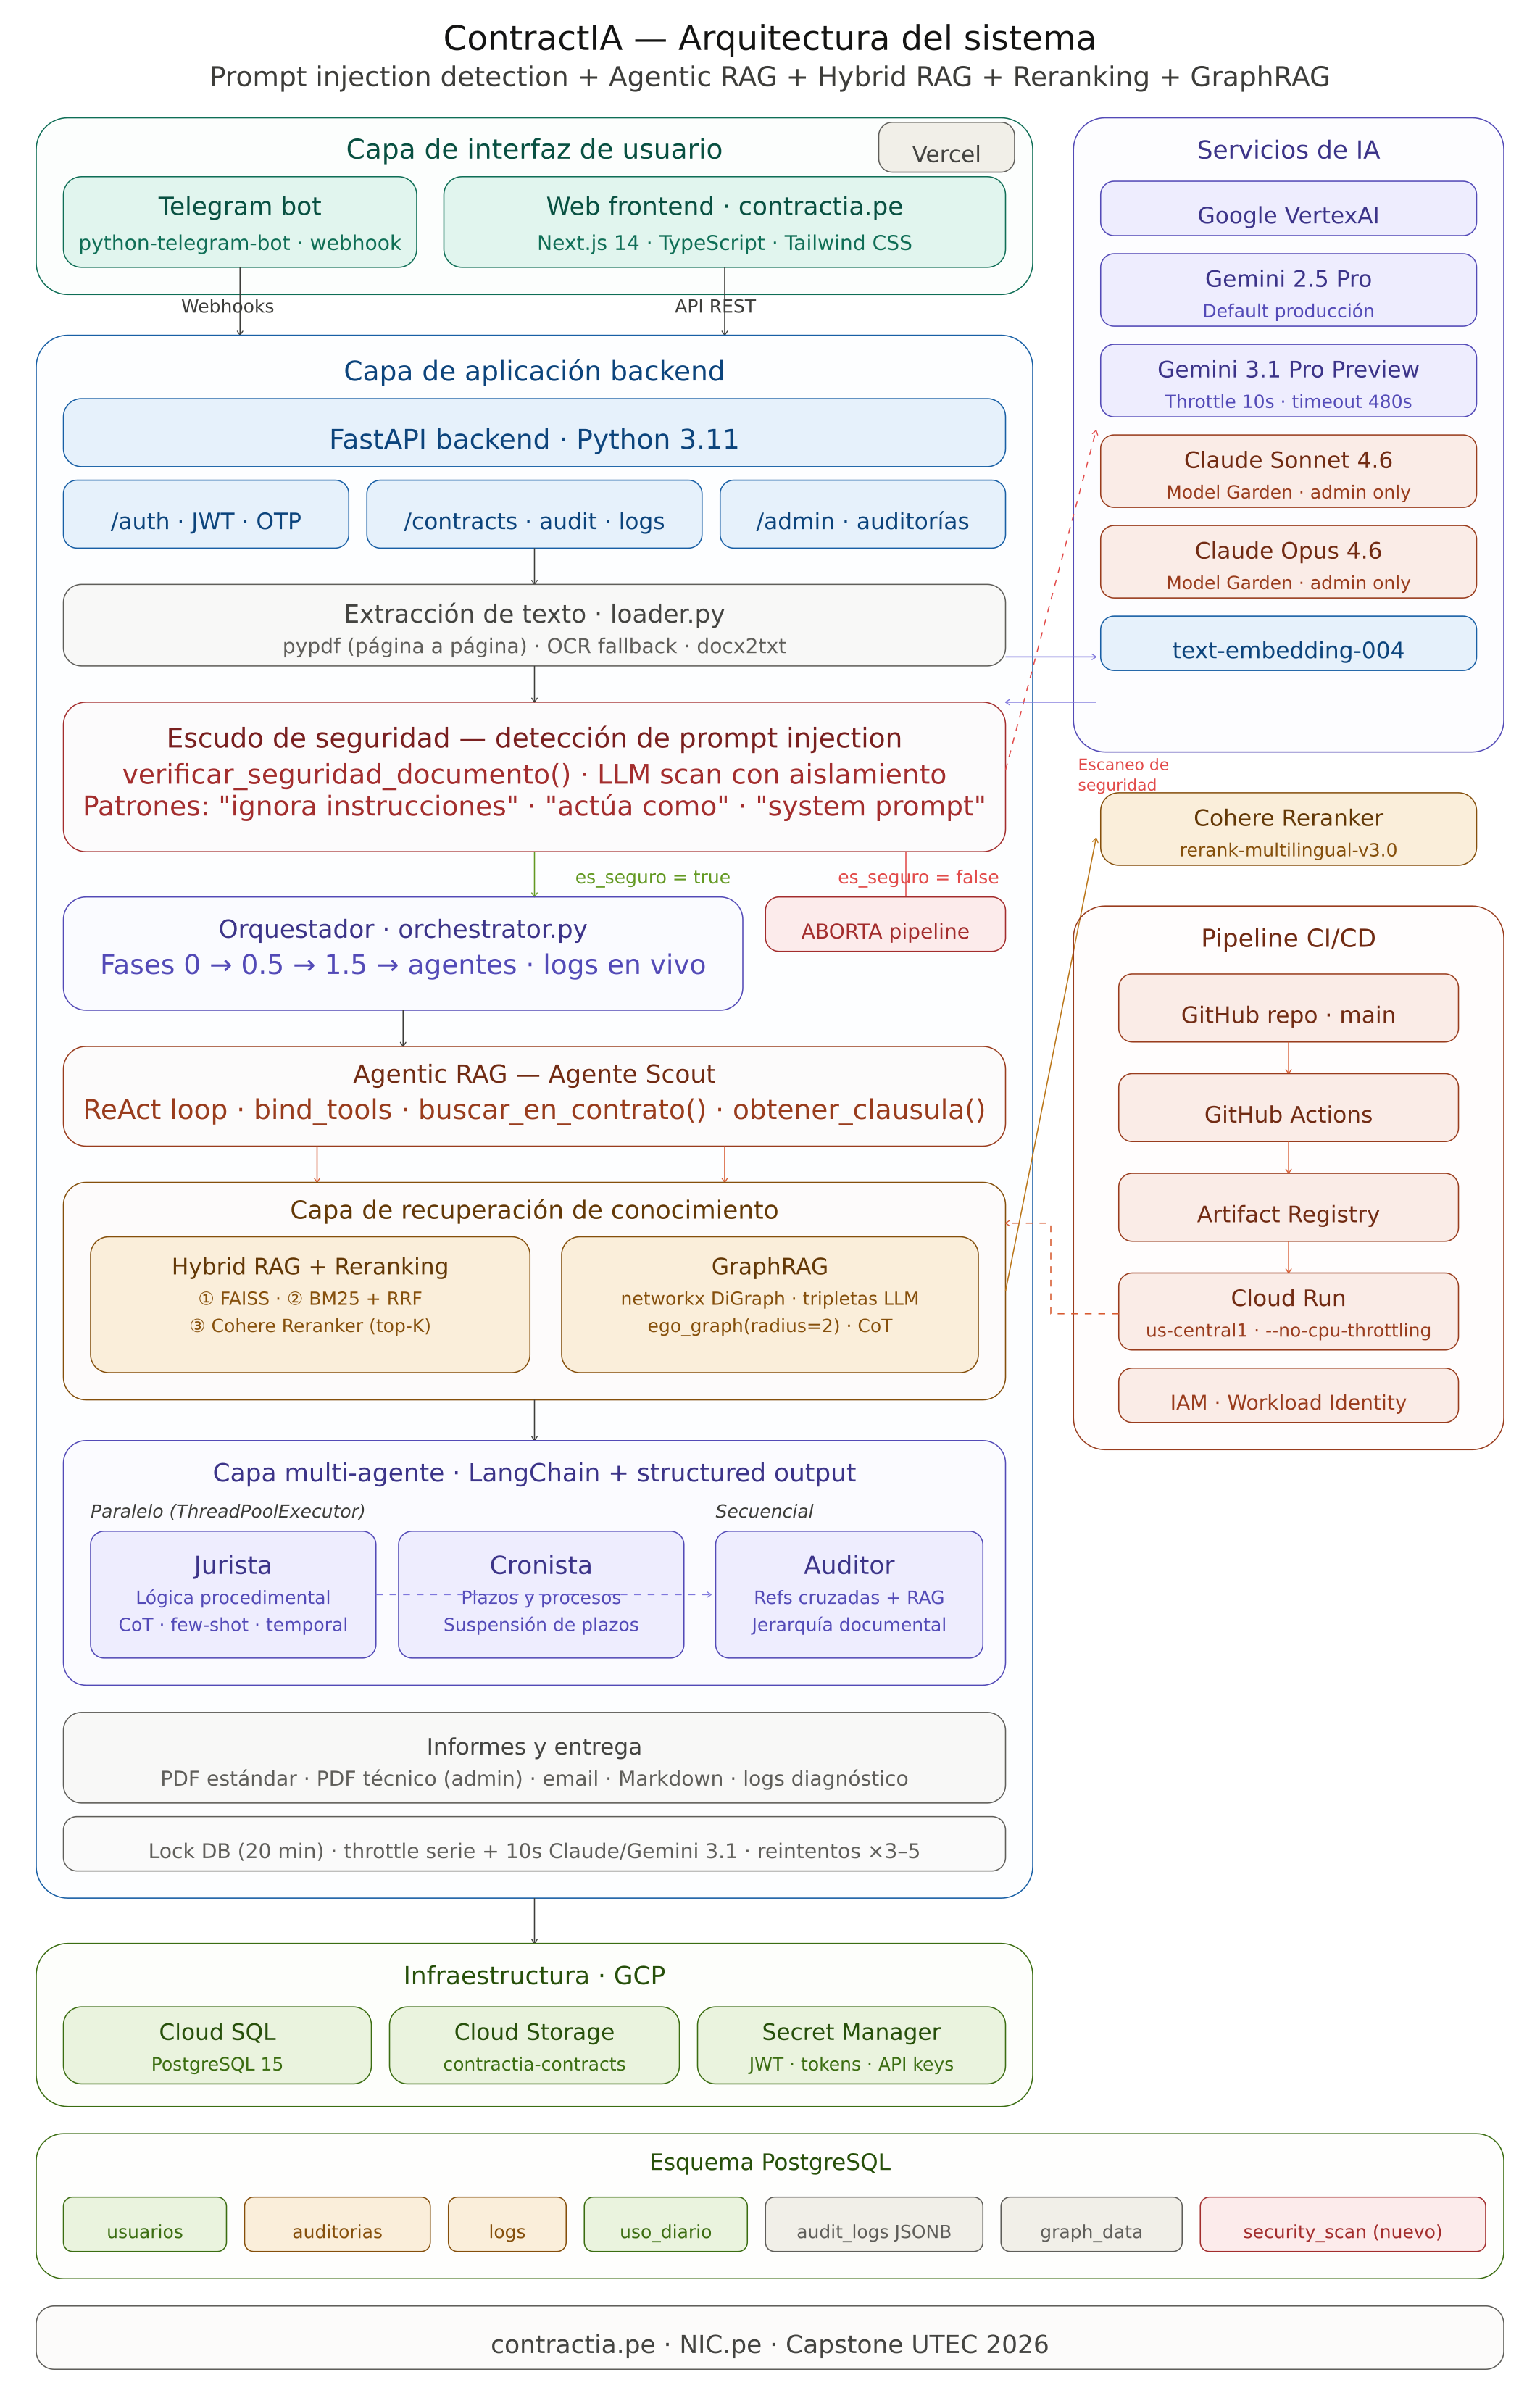
\includegraphics[width=0.87\linewidth]{images/contractia_architecture_centered.png}
    \caption{Arquitectura Detallada}
    \label{fig:Arquitectura Detallada}
\end{figure}

% ─────────────────────────────────────────────────────────────────────────────
\section{Flujo de Procesamiento End-to-End}

El pipeline de auditoría sigue un flujo secuencial de fases bien definidas,
ejecutadas de forma autónoma tras la carga del contrato:

\begin{table}[H]
\centering
\caption{Fases del pipeline de auditoría ContractIA}
\label{tab:pipeline}
\begin{tabular}{p{0.5cm} p{3.5cm} p{4.5cm} p{5cm}}
\toprule
\textbf{\#} & \textbf{Fase} & \textbf{Componente} & \textbf{Resultado} \\
\midrule
0 & Segmentación & Regex + Anti-TOC & 41 secciones (contrato piloto) \\[3pt]
0.5 & Indexación multinivel & FAISS + índice global & 448 cláusulas indexadas \\[3pt]
1 & RAG híbrido & FAISS + BM25 + Cohere & Contexto normativo por sección \\[3pt]
1.5 & GraphRAG & NetworkX DiGraph + LLM & Grafo de relaciones contractuales \\[3pt]
2 & Análisis multi-agente & Jurista + Auditor + Cronista & Hallazgos trazados por sección \\[3pt]
3 & Consolidación & Orquestador + Pydantic & Reporte JSON estructurado \\[3pt]
4 & Generación de reporte & FastAPI + Cloud Storage & PDF ejecutivo descargable \\[3pt]
5 & Notificación & Email automático & Aviso al usuario al finalizar \\
\bottomrule
\end{tabular}
\end{table}

% ─────────────────────────────────────────────────────────────────────────────
\section{Capa de Ingesta}

El sistema recibe contratos a través de dos canales: la API REST (carga
directa vía frontend web) y el bot Telegram (carga conversacional). El
proceso de ingesta comprende:

\begin{itemize}
    \item \textbf{Extracción de texto:} PyMuPDF como extractor principal,
    con \textit{pdfminer} como fallback para PDFs con estructura compleja.
    Normalización UTF-8 y detección de páginas ilegibles o con OCR defectuoso.
    \item \textbf{Almacenamiento:} El contrato se persiste en Google Cloud
    Storage con un identificador único de auditoría. El registro de la
    auditoría se crea en PostgreSQL con estado \texttt{pendiente}.
    \item \textbf{Cola de trabajos:} Cada usuario puede tener hasta 5 trabajos
    pendientes. El sistema procesa un contrato activo a la vez por usuario;
    los demás quedan en cola y se procesan secuencialmente.
\end{itemize}

% ─────────────────────────────────────────────────────────────────────────────
\section{Pipeline de Procesamiento Estructural}

\subsection{FASE 0 — Segmentación automática}

El segmentador identifica capítulos y anexos mediante expresiones regulares
calibradas para contratos de concesión peruanos. Incluye:

\begin{itemize}
    \item \textbf{Mecanismo anti-TOC:} Filtra títulos duplicados originados
    en las tablas de contenido del documento, evitando secciones fantasma
    con cero cláusulas.
    \item \textbf{Resolución por densidad:} Cuando dos secciones compiten
    por el mismo título, prevalece la de mayor densidad de cláusulas.
    \item \textbf{Resultado en contrato piloto:} 20 capítulos + 21 anexos
    = 41 secciones con cobertura del 100\%.
\end{itemize}

\subsection{FASE 0.5 — Indexación multinivel}

Se construyen tres índices complementarios para soportar el análisis:

\begin{itemize}
    \item \textbf{Índice Global de Cláusulas:} Mapeo de todas las cláusulas
    del contrato con su número, sección y texto. El contrato piloto produjo
    448 entradas.
    \item \textbf{Índice de Secciones:} Metadatos de cada sección (título,
    rango de páginas, número de cláusulas).
    \item \textbf{Índice Local por sección:} Permite búsqueda de cláusulas
    dentro del contexto de una sección específica durante el análisis.
\end{itemize}

\subsection{FASE 1 — RAG Híbrido}

El módulo RAG combina tres estrategias de recuperación para maximizar la
relevancia del contexto normativo:

\begin{itemize}
    \item \textbf{FAISS (semántico):} Vectorización con
    \texttt{text-embedding-004} (Vertex~AI, 768 dimensiones). Recuperación
    por similitud coseno sobre la base normativa vectorizada (Ley de APP,
    TUO de Contrataciones, normas OSITRAN, OSINERGMIN, SUNASS).
    \item \textbf{BM25 (léxico):} Captura coincidencias exactas de términos
    legales, números de artículo y denominaciones específicas que los
    embeddings semánticos pueden subestimar.
    \item \textbf{Cohere Rerank v3:} Reordena los fragmentos recuperados por
    ambos métodos según su relevancia contextual real, reduciendo el ruido
    en el contexto enviado al LLM.
\end{itemize}

\subsection{FASE 1.5 — GraphRAG}

El módulo GraphRAG enriquece el análisis con contexto relacional:

\begin{itemize}
    \item \textbf{Extracción de tripletas:} El LLM extrae relaciones del tipo
    (origen, tipo\_relación, destino) por sección. Tipos de relación:
    \texttt{REFERENCIA\_A}, \texttt{ESTABLECE\_PLAZO}, \texttt{MODIFICA\_A},
    \texttt{DEPENDE\_DE}, \texttt{OBLIGA\_A}.
    \item \textbf{Grafo DiGraph (NetworkX):} El contrato piloto generó entre
    208 y 477 nodos y entre 258 y 617 relaciones, según el modelo empleado.
    \item \textbf{Uso en auditoría:} El orquestador consulta el grafo para
    identificar qué otras secciones tienen relaciones con la sección bajo
    análisis, enriqueciendo el contexto de cada agente.
\end{itemize}

% ─────────────────────────────────────────────────────────────────────────────
\section{Motor Multi-Agente (FASE 2)}

El núcleo analítico de ContractIA son tres agentes especializados que operan
en paralelo sobre cada sección del contrato:

\begin{table}[H]
\centering
\caption{Agentes especializados del motor de auditoría}
\label{tab:agentes}
\begin{tabular}{p{2.5cm} p{5cm} p{6cm}}
\toprule
\textbf{Agente} & \textbf{Especialización} & \textbf{Tipos de hallazgo} \\
\midrule
\textbf{Jurista} &
  Coherencia legal y semántica entre cláusulas &
  Contradicciones entre obligaciones, referencias semánticas incorrectas,
  ambigüedades en definiciones, omisiones normativas \\[4pt]
\textbf{Auditor} &
  Validación estructural y referencias cruzadas &
  Referencias a cláusulas inexistentes, numeración inconsistente,
  definiciones no utilizadas, secciones huérfanas \\[4pt]
\textbf{Cronista} &
  Coherencia temporal y de plazos &
  Plazos contradictorios, secuencias de hitos imposibles,
  inconsistencias en fechas de vigencia \\
\bottomrule
\end{tabular}
\end{table}

El \textbf{Orquestador} coordina la ejecución de los tres agentes mediante
\texttt{asyncio.gather}, consolida sus hallazgos eliminando duplicados y
aplica clasificación de severidad automática (ALTA / MEDIA / BAJA).
Los agentes utilizan \texttt{with\_structured\_output} de LangChain~0.3+
con esquemas Pydantic para garantizar salida JSON reproducible y tipada.

Para modelos LLM con cuota restringida (Claude~Sonnet, Gemini~3.1~Pro
Preview), el sistema aplica ejecución en serie con pausa de 30~s entre
llamadas para evitar errores 429.

% ─────────────────────────────────────────────────────────────────────────────
\section{Capa de Servicios e Infraestructura}

\begin{itemize}
    \item \textbf{API REST (FastAPI + Python~3.11):} Hub central con
    endpoints para carga de contratos, inicio y seguimiento de auditorías,
    consulta de estado por polling, descarga de reportes y administración
    de usuarios. Autenticación JWT con cuatro roles:
    \texttt{pendiente / básico / auditor / admin}.
    \item \textbf{Google Cloud Run:} Servicio containerizado con auto-scaling
    y disponibilidad $\geq 99\%$. Imagen Docker almacenada en Artifact
    Registry; despliegue continuo vía GitHub Actions con Workload Identity
    Federation (sin credenciales estáticas).
    \item \textbf{Cloud SQL (PostgreSQL~15):} Persistencia de auditorías,
    hallazgos individuales, logs de procesamiento y gestión de usuarios.
    Conexión segura vía Cloud SQL Auth Proxy.
    \item \textbf{Google Cloud Storage:} Almacenamiento de contratos PDF/DOCX
    cargados y reportes ejecutivos generados, con URLs firmadas de descarga.
    \item \textbf{Secret Manager:} Gestión centralizada de credenciales
    (API keys de Vertex~AI, Cohere, JWT secret) sin exposición en código
    ni variables de entorno en texto plano.
\end{itemize}

% ─────────────────────────────────────────────────────────────────────────────
\section{Interfaces de Usuario}

\begin{itemize}
    \item \textbf{Frontend web (Next.js~14, TypeScript, Tailwind CSS):}
    Dashboard de auditorías con panel de diagnóstico técnico en tiempo real
    (polling SSE), visualización de hallazgos por severidad, descarga de
    reportes PDF. Desplegado en \texttt{contractia.pe} vía Vercel.
    \item \textbf{Bot Telegram (python-telegram-bot~20+):} Interfaz
    conversacional para carga de contratos, seguimiento de progreso en cola,
    descarga de reportes y gestión de accesos (aprobación de nuevos usuarios
    por el administrador). Opera en modo webhook sobre Cloud Run.
    Notificación automática por email al usuario al finalizar el análisis.
\end{itemize}

% ─────────────────────────────────────────────────────────────────────────────
\section{Stack Tecnológico}

\begin{table}[H]
\centering
\caption{Stack tecnológico del MVP ContractIA}
\label{tab:stack}
\begin{tabular}{p{4cm} p{9.5cm}}
\toprule
\textbf{Componente} & \textbf{Tecnología} \\
\midrule
LLM principal       & Gemini 2.5 Pro (Vertex AI) \\
LLM alternativo     & Gemini 3.1 Pro Preview / Claude Sonnet 4.6 \\
Embeddings          & text-embedding-004 (Vertex AI, 768 dim.) \\
Vector store        & FAISS (índice local por auditoría) \\
Búsqueda léxica     & BM25 (rank-bm25) \\
Reranker            & Cohere Rerank v3 \\
Grafo de conocimiento & NetworkX DiGraph \\
Orquestación LLM    & LangChain 0.3+ (LCEL, PromptTemplate, Pydantic) \\
Backend API         & FastAPI + Python 3.11 + Uvicorn \\
Base de datos       & PostgreSQL 15 (Google Cloud SQL) \\
Almacenamiento      & Google Cloud Storage \\
Secretos            & Google Secret Manager \\
Despliegue          & Google Cloud Run (auto-scaling) \\
Frontend            & Next.js 14 (TypeScript + Tailwind CSS) — Vercel \\
Bot                 & Telegram Bot API (python-telegram-bot 20+) \\
CI/CD               & GitHub Actions + Workload Identity Federation \\
\bottomrule
\end{tabular}
\end{table}

% ─────────────────────────────────────────────────────────────────────────────
\section{Decisiones de Diseño y Justificación}

Las siguientes decisiones de arquitectura tuvieron implicaciones directas
sobre el rendimiento, costo y mantenibilidad del sistema:

\begin{enumerate}
    \item \textbf{Agentes en paralelo con fallback en serie:}
    Los tres agentes se ejecutan con \texttt{asyncio.gather} para minimizar
    la latencia total. Para modelos con cuotas restringidas se aplica
    ejecución en serie con pausa de 30~s. Esta decisión reduce el tiempo
    de análisis en $\sim$66\% respecto a ejecución puramente secuencial.

    \item \textbf{RAG híbrido (BM25 + FAISS) sobre solo-vectorial:}
    Los embeddings semánticos tienden a subestimar coincidencias exactas de
    términos técnicos legales (``Artículo 15.3'', ``Cláusula de penalidad'').
    BM25 complementa con recuperación léxica precisa, y Cohere Reranker
    fusiona y reordena ambos resultados. Esta combinación mejoró la
    precisión del contexto RAG en pruebas internas.

    \item \textbf{GraphRAG como contexto relacional adicional:}
    El grafo de conocimiento permite que el análisis de una sección incorpore
    información de otras secciones vinculadas por relaciones contractuales,
    mejorando la detección de inconsistencias entre cláusulas distantes.
    No reemplaza al RAG normativo; lo complementa con contexto intra-contrato.

    \item \textbf{Polling sobre Server-Sent Events (SSE):}
    Cloud Run no soporta conexiones SSE persistentes sin un proxy nginx
    adicional. El panel de diagnóstico técnico del frontend implementa
    polling cada 5~s sobre el endpoint de logs, logrando el efecto visual
    de actualización en tiempo real sin infraestructura adicional.

    \item \textbf{Cola por usuario sobre semáforo global:}
    En lugar de un semáforo global (un trabajo en todo el sistema), cada
    usuario tiene su propia cola con un máximo de 5 trabajos. Esto permite
    que múltiples usuarios usen el sistema sin bloquearse mutuamente,
    mientras se mantiene el control de costos de API por usuario.

    \item \textbf{Secret Manager sobre variables de entorno:}
    Las credenciales de Vertex~AI, Cohere y JWT se gestionan en Secret
    Manager en lugar de variables de entorno en texto plano en Cloud Run.
    Esto elimina el riesgo de exposición de credenciales en logs y
    simplifica la rotación de claves sin redeploy.
\end{enumerate}
%% ── 8. DESARROLLO Y CONSTRUCCIÓN ─────────────────────────────────────────────
\chapter{Desarrollo y Construcción}

Este capítulo documenta el proceso de desarrollo de ContractIA, desde los
primeros experimentos en notebooks hasta el MVP desplegado en producción.
El desarrollo siguió un enfoque iterativo e incremental, con 15 versiones
de notebook (prototipo) y 4 versiones de plataforma (MVP), priorizando en
cada ciclo la hipótesis de mayor riesgo técnico pendiente de validar.

\section{Enfoque Metodológico}

El desarrollo adoptó un ciclo corto de construcción–medición–aprendizaje
(\textit{build–measure–learn}), con las siguientes decisiones de proceso:

\begin{itemize}
    \item \textbf{Iteraciones cortas (2--5 días):} cada versión del notebook
    resolvía un problema específico antes de agregar nueva funcionalidad.
    \item \textbf{Contrato piloto fijo:} el contrato A
    (324 páginas) fue el benchmark constante entre iteraciones, permitiendo
    comparaciones objetivas de cobertura, tiempo y hallazgos.
    \item \textbf{Separación prototipo / MVP:} las iteraciones v1--v15 se
    desarrollaron en Jupyter como exploración analítica; la plataforma
    productiva (FastAPI + Cloud Run) se construyó en paralelo a partir de v9.5.
    \item \textbf{Validación continua:} tras cada iteración se revisó
    manualmente una muestra de 10--20 hallazgos para detectar regresiones.
\end{itemize}

\section{Historial de Versiones}

\begin{table}[H]
\centering
\caption{Evolución de versiones del sistema ContractIA}
\label{tab:versiones}
\begin{tabular}{p{2cm} p{3.5cm} p{7cm}}
\toprule
\textbf{Versión} & \textbf{Hito} & \textbf{Cambio principal} \\
\midrule
v1.0  & Pipeline base      & Segmentación PDF + FAISS + 1 agente LLM \\
v2--v4 & Calidad RAG       & Chunking adaptativo; filtrado anti-TOC \\
v5    & Multi-agente       & Jurista + Auditor + Cronista con Pydantic \\
v6--v7 & Orquestación      & \texttt{asyncio.gather}; trazabilidad por cláusula \\
v8.7  & Hybrid RAG         & BM25 + FAISS fusión RRF \\
v8.8  & Cohere Reranker    & Cross-encoder sobre top-20 candidatos \\
v9.0  & GraphRAG           & DiGraph por sección; extracción de tripletas LLM \\
v9.5  & API + Cloud Run    & FastAPI; Docker; CI/CD con GitHub Actions \\
v9.6  & Telegram bot       & Webhook; flujo de aprobación de usuarios \\
v9.7  & Frontend Next.js   & Panel web; polling de estado en tiempo real \\
v9.8  & Cola + notif.      & Cola por usuario (máx. 5 trabajos); email al finalizar \\
\bottomrule
\end{tabular}
\end{table}

\section{Iteraciones del Desarrollo}

\subsection{Iteración 1 — Prototipo en Notebook (v1.0--v4)}

\textbf{Objetivo:} validar que un LLM puede identificar inconsistencias
contractuales en un contrato de concesión peruano real.

\textbf{Construcción:}
\begin{itemize}
    \item Extracción de texto con PyMuPDF y segmentación por jerarquía
    de capítulos y cláusulas (regex + heurísticas).
    \item Indexación de fragmentos en FAISS con embeddings
    \texttt{text-embedding-004} de Vertex AI.
    \item Un único agente LLM (Gemini 2.5 Pro) con prompt de análisis
    semántico e instrucción de devolver JSON estructurado.
    \item Iteraciones v2--v4: mejora del chunking adaptativo para evitar
    que el índice de contenido (TOC) sea indexado como cláusula.
\end{itemize}

\textbf{Desafío clave:} el módulo anti-TOC era crítico; sin él, el RAG
recuperaba fragmentos del índice del contrato en lugar de cláusulas reales,
generando hallazgos sin sustento.

\textbf{Resultado:} 35 inconsistencias detectadas sobre el Contrato A
(314 páginas) en 47 minutos. Validó la hipótesis central de viabilidad técnica.

\subsection{Iteración 2 — Arquitectura Multi-Agente (v5--v7)}

\textbf{Objetivo:} aumentar la cobertura y especialización del análisis
descomponiendo el agente único en roles diferenciados.

\textbf{Construcción:}
\begin{itemize}
    \item \textbf{Jurista:} analiza consistencia con normativa (D.Leg.\ 1362,
    guías ProInversión). Devuelve \texttt{HallazgoJurista} con campo
    \texttt{referencia\_normativa}.
    \item \textbf{Auditor:} detecta contradicciones internas, referencias
    cruzadas rotas y omisiones entre secciones. Devuelve
    \texttt{HallazgoAuditor} con \texttt{seccion\_referenciada}.
    \item \textbf{Cronista:} identifica conflictos de fechas, plazos
    inconsistentes y hitos mal ordenados. Devuelve \texttt{HallazgoCronista}
    con \texttt{fecha\_detectada} y \texttt{fecha\_esperada}.
    \item Orquestador con \texttt{asyncio.gather} para ejecutar los tres
    agentes en paralelo por sección, reduciendo la latencia total.
    \item Esquemas de salida con Pydantic v2 para garantizar estructura
    consistente y validación automática de tipos.
\end{itemize}

\textbf{Desafío clave:} alinear el formato de salida JSON de tres agentes
distintos en un único consolidado por sección, evitando duplicados y
asignando correctamente el índice global de hallazgo.

\textbf{Resultado:} incremento de cobertura temática; hallazgos clasificados
por tipo (jurídico, estructural, temporal) con trazabilidad completa.

\subsection{Iteración 3 — RAG Híbrido y GraphRAG (v8--v9)}

\textbf{Objetivo:} mejorar la relevancia del contexto normativo recuperado
y enriquecer el análisis con relaciones entre secciones del contrato.

\textbf{Construcción:}
\begin{itemize}
    \item \textbf{Hybrid RAG (v8.7):} fusión de BM25 (recuperación léxica)
    y FAISS (recuperación semántica) mediante Reciprocal Rank Fusion (RRF),
    mejorando la cobertura sobre términos legales técnicos poco frecuentes.
    \item \textbf{Cohere Reranker (v8.8):} cross-encoder sobre los
    top-20 candidatos del RAG híbrido para seleccionar los 5 más relevantes,
    reduciendo ruido en el contexto entregado a los agentes.
    \item \textbf{GraphRAG (v9.0):} extracción de tripletas
    \textit{(sujeto, relación, objeto)} por sección mediante LLM;
    construcción de un \texttt{DiGraph} (NetworkX) por contrato con
    relaciones: \texttt{obliga\_a}, \texttt{referencia}, \texttt{modifica},
    \texttt{contradice}, \texttt{complementa}. Permite consultar vecinos
    de un nodo para enriquecer el contexto de análisis cruzado.
\end{itemize}

\textbf{Desafío clave:} la extracción de tripletas con LLM es costosa
(1 llamada adicional por sección); se implementó caché por hash de sección
para evitar reextracción en análisis sucesivos del mismo contrato.

\textbf{Resultado:} reducción de falsos positivos por contexto irrelevante;
detección de contradicciones entre secciones no adyacentes gracias al grafo.

\subsection{Iteración 4 — Despliegue en Producción (v9.5--v9.8)}

\textbf{Objetivo:} convertir el notebook analítico en un servicio accesible,
operativo y escalable para usuarios no técnicos.

\textbf{Construcción:}
\begin{itemize}
    \item \textbf{API FastAPI (v9.5):} encapsulamiento del pipeline de
    auditoría como servicio HTTP con endpoints \texttt{/contracts/upload},
    \texttt{/contracts/\{id\}/audit} y \texttt{/contracts/\{id\}/status}.
    Containerización con Docker; imagen publicada en Artifact Registry.
    CI/CD con GitHub Actions: build → push → deploy a Cloud Run en cada
    merge a \texttt{main}.
    \item \textbf{Bot Telegram (v9.6):} webhook en \texttt{/telegram/webhook};
    flujo de registro, aprobación por administrador (rol \texttt{auditor})
    y comandos \texttt{/upload}, \texttt{/status}, \texttt{/report}.
    \item \textbf{Frontend Next.js (v9.7):} panel web en
    \texttt{contractia.pe}; autenticación JWT; subida de contratos;
    visualización de hallazgos con filtro por tipo y severidad;
    polling de estado en tiempo real (actualización cada 10 segundos).
    \item \textbf{Cola y notificación (v9.8):} sistema de cola por usuario
    con máximo 5 trabajos pendientes; procesamiento secuencial en segundo
    plano; notificación por correo electrónico al finalizar el análisis.
\end{itemize}

\textbf{Desafío clave:} garantizar que el análisis de un contrato extenso
(análisis completo: $\approx 75$ minutos) no bloqueara el hilo principal
de la API; solución: \texttt{BackgroundTasks} de FastAPI con persistencia
de estado en Cloud SQL.

\textbf{Resultado:} MVP funcional en producción en \texttt{contractia.pe},
accesible vía web y Telegram, con análisis completo del Contrato A
en $\approx 1$ hora 15 minutos con Gemini~2.5~Pro.

\section{Dataset Utilizado}

\begin{table}[H]
\centering
\caption{Datasets empleados en el desarrollo y validación del MVP}
\label{tab:datasets}
\begin{tabular}{p{3.5cm} p{9.5cm}}
\toprule
\textbf{Dataset} & \textbf{Descripción} \\
\midrule
Contrato piloto &
    Contrato A (ProInversión): 324 páginas, 41 secciones,
    448 cláusulas, 749{,}499 caracteres. Usado como benchmark
    constante entre iteraciones. \\
Corpus de segmentación &
    17 contratos de concesión de ProInversión de distintos sectores
    (agua, energía, vial), extensión variable. Usados exclusivamente
    para pruebas de robustez del módulo anti-TOC y segmentación. \\
Base normativa &
    Guías institucionales de ProInversión, D.Leg.\ 1362 y su
    Reglamento, normativa sectorial complementaria; vectorizados
    en FAISS e indexados en BM25. Total: $\approx 1{,}200$ fragmentos
    normativos. \\
\bottomrule
\end{tabular}
\end{table}

\section{Modelos Implementados y Evaluados}

\begin{table}[H]
\centering
\caption{Modelos LLM evaluados en ContractIA}
\label{tab:modelos}
\begin{tabular}{p{3.8cm} p{2.5cm} p{6.5cm}}
\toprule
\textbf{Modelo} & \textbf{Estado} & \textbf{Observación} \\
\midrule
Gemini 2.5 Pro (Vertex AI) & \textbf{Producción} &
    Velocidad óptima ($\approx 75$ min para 41 secciones); 119
    hallazgos sobre Contrato A; balance costo/cobertura. \\
Gemini 3.1 Pro Preview      & Evaluación &
    Mayor riqueza del grafo de conocimiento; 55 hallazgos en
    benchmark preliminar; mayor latencia ($\approx 3$ h 10 min). \\
Claude Sonnet 4.6 / Opus 4.6 & Pendiente &
    Integrado vía Vertex AI; en evaluación de cuota; resultados
    preliminares prometedores en análisis semántico. \\
\bottomrule
\end{tabular}
\end{table}

\section{Desafíos Técnicos y Soluciones}

Durante el desarrollo se enfrentaron tres desafíos técnicos principales:

\begin{enumerate}
    \item \textbf{Variabilidad en la estructura del PDF:}
    Los contratos de ProInversión usan numeraciones inconsistentes,
    tablas anidadas y TOC de múltiples páginas. Solución: módulo anti-TOC
    basado en detección estadística de densidad de referencias numéricas;
    heurística de longitud mínima de fragmento ($> 200$ caracteres) para
    filtrar entradas del índice.

    \item \textbf{Límite de contexto de los LLMs:}
    Cláusulas muy extensas exceden la ventana de contexto óptima.
    Solución: truncamiento adaptativo al 80\% del límite del modelo,
    preservando la cabecera de la cláusula y el párrafo más relevante
    según el score del Reranker.

    \item \textbf{Consistencia entre ejecuciones:}
    Los LLMs generativos producen variaciones entre ejecuciones con el
    mismo input. Solución: temperatura fija a 0.1 en todos los agentes;
    esquemas Pydantic con validación estricta de tipos; postprocesamiento
    de deduplicación por similitud de texto ($> 0.9$ cosine similarity).

    \item \textbf{Gestión de secretos y seguridad en producción:}
    Credenciales de API (Vertex AI, Cohere, PostgreSQL, SMTP) no pueden
    residir en el código ni en el Dockerfile. Solución: todas las
    credenciales almacenadas en Google Cloud Secret Manager; el servicio
    las lee en tiempo de ejecución mediante la service account
    \texttt{contractia-sa}; el Dockerfile no contiene ningún secreto.

    \item \textbf{Análisis de larga duración sin bloquear la API:}
    Un análisis completo toma $\approx 75$ minutos; un endpoint síncrono
    agotaría el timeout de Cloud Run (máx. 60 min por defecto) y bloquearía
    la respuesta al usuario. Solución: endpoint \texttt{/audit} dispara un
    \texttt{BackgroundTask} y devuelve inmediatamente el \texttt{job\_id};
    el cliente consulta el estado vía polling en \texttt{/status}; al
    finalizar el backend envía notificación por correo electrónico.
\end{enumerate}

\section{Estructura del Repositorio}

El código del MVP está organizado en dos capas principales: la lógica analítica
(\texttt{contractia/}) y la capa de servicio (\texttt{api/}), con separación
clara de responsabilidades.

\begin{longtable}{p{5cm} p{9cm}}
\caption{Módulos principales del repositorio ContractIA}
\label{tab:repo} \\
\toprule
\textbf{Módulo / Archivo} & \textbf{Responsabilidad} \\
\midrule
\endfirsthead
\multicolumn{2}{l}{\small\itshape Continuación de la Tabla~\ref{tab:repo}} \\[4pt]
\toprule
\textbf{Módulo / Archivo} & \textbf{Responsabilidad} \\
\midrule
\endhead
\midrule
\multicolumn{2}{r}{\small\itshape Continúa en la siguiente página} \\
\endfoot
\bottomrule
\endlastfoot
\texttt{contractia/config.py} &
    Variables de entorno, flags de feature (\texttt{RAG\_ENABLED},
    \texttt{GRAPHRAG\_ENABLED}, \texttt{AGENTIC\_RAG\_ENABLED}),
    modelos LLM configurables. \\[6pt]
\texttt{contractia/pipeline.py} &
    Orquestación de las fases FASE~0 a FASE~5: segmentación,
    indexación, RAG, agentes, consolidación, reporte. \\[6pt]
\texttt{contractia/orchestrator.py} &
    Función \texttt{auditar\_consistencia()} por sección;
    gestión de contexto RAG y llamadas a agentes. \\[6pt]
\texttt{contractia/agents/} &
    Fábrica de agentes (\texttt{factory.py}); clases
    \texttt{AgenteJurista}, \texttt{AgenteAuditor},
    \texttt{AgenteCronista}; schemas Pydantic por agente. \\[6pt]
\texttt{contractia/rag/} &
    Módulos FAISS, BM25, Cohere Reranker, GraphRAG (NetworkX);
    función unificada \texttt{recuperar\_contexto()}. \\[6pt]
\texttt{contractia/segmentation/} &
    Extracción PDF (PyMuPDF + pdfminer), anti-TOC,
    segmentador jerárquico, normalización de texto. \\[6pt]
\texttt{contractia/reports/} &
    Generación de reporte ejecutivo PDF (FPDF2);
    consolidación y deduplicación de hallazgos. \\[6pt]
\texttt{api/main.py} &
    Entrada FastAPI; registro de routers;
    endpoint de salud \texttt{/health}. \\[6pt]
\texttt{api/routers/} &
    \texttt{auth\_router} (JWT), \texttt{contracts\_router}
    (upload, audit, status, report), \texttt{admin\_router}
    (gestión de usuarios y roles). \\[6pt]
\texttt{contractia/telegram/} &
    Handler del bot; comandos; flujo de aprobación;
    wrapper psycopg2 para Cloud SQL. \\[6pt]
\texttt{Dockerfile} &
    Imagen Python 3.11 slim; sin secretos embebidos;
    \texttt{ENTRYPOINT} Uvicorn. \\[6pt]
\texttt{.github/workflows/deploy.yml} &
    Pipeline CI/CD: build → push a Artifact Registry →
    deploy a Cloud Run (Workload Identity Federation). \\
\end{longtable}

\section{Infraestructura y Pipeline CI/CD}

La infraestructura del MVP está desplegada íntegramente en Google Cloud
Platform, organizada en los siguientes servicios:

\begin{itemize}
    \item \textbf{Cloud Run:} servicio sin servidor (\textit{serverless})
    que ejecuta el contenedor Docker del API; escala automáticamente a
    cero cuando no hay tráfico, reduciendo costos operativos.
    \item \textbf{Cloud SQL (PostgreSQL 15):} base de datos relacional
    para usuarios, roles, jobs de análisis y metadatos de contratos.
    Acceso desde Cloud Run mediante el conector oficial de Cloud SQL.
    \item \textbf{Cloud Storage:} almacenamiento de contratos PDF subidos
    por los usuarios y reportes generados; acceso con signed URLs de
    duración limitada para descarga segura.
    \item \textbf{Artifact Registry:} registro de imágenes Docker;
    versiones inmutables por cada build del CI/CD.
    \item \textbf{Secret Manager:} almacén centralizado de credenciales
    (Vertex AI, Cohere, PostgreSQL, SMTP, JWT secret); sin secretos
    en variables de entorno del Dockerfile.
    \item \textbf{Vertex AI:} API administrada de Google para Gemini 2.5
    Pro (inferencia LLM) y \texttt{text-embedding-004} (embeddings);
    facturación por token, sin infraestructura de GPU propia.
\end{itemize}

El pipeline CI/CD ejecuta los siguientes pasos en cada \textit{merge} a la
rama \texttt{main}:

\begin{enumerate}
    \item \textbf{Checkout y autenticación:} obtención del token de acceso
    a GCP mediante Workload Identity Federation (sin clave de servicio
    almacenada en GitHub Secrets).
    \item \textbf{Build Docker:} construcción de la imagen con tag
    \texttt{git SHA} para trazabilidad de versiones.
    \item \textbf{Push a Artifact Registry:} imagen disponible en
    \texttt{us-central1-docker.pkg.dev/striking-domain-488917-p8/contractia/api}.
    \item \textbf{Deploy a Cloud Run:} actualización del servicio
    \texttt{contractia-api} con la nueva imagen; Cloud Run realiza
    \textit{rolling deployment} sin downtime.
    \item \textbf{Verificación de salud:} el workflow consulta
    \texttt{/health} y falla el deploy si no responde HTTP~200.
\end{enumerate}

\section{Estrategia de Pruebas y Validación}

La validación del sistema se realizó en tres niveles complementarios:

\begin{enumerate}
    \item \textbf{Validación funcional por iteración:}
    Tras cada versión de notebook se ejecutó el análisis completo sobre
    el contrato A y se comparó el conteo de hallazgos,
    tipos detectados y tiempo de procesamiento con la versión anterior.
    Cualquier regresión ($> 10\%$ de reducción en hallazgos) bloqueaba
    el avance a la siguiente iteración.

    \item \textbf{Validación manual de calidad semántica:}
    Una muestra aleatoria de 30 hallazgos de severidad ALTA fue revisada
    por dos especialistas legales independientes. Cada hallazgo fue
    clasificado como verdadero positivo (TP), falso positivo (FP) o
    falso negativo (FN). La precisión estimada resultante fue $\approx 87\%$.

    \item \textbf{Pruebas de integración del MVP:}
    Antes del despliegue en producción se verificaron manualmente:
    \begin{itemize}
        \item Subida de PDF vía API y vía bot Telegram.
        \item Flujo completo de análisis en segundo plano y consulta de estado.
        \item Generación y descarga del reporte ejecutivo PDF.
        \item Flujo de aprobación de usuario y cambio de rol.
        \item Cola de trabajos: llegada al límite de 5 y rechazo del 6.º.
        \item Notificación por correo al finalizar el análisis.
    \end{itemize}
\end{enumerate}

\begin{table}[H]
\centering
\caption{Resumen de resultados de validación por iteración}
\label{tab:validacion_iter}
\begin{tabular}{p{3cm} p{2.8cm} p{2.2cm} p{4.5cm}}
\toprule
\textbf{Versión} & \textbf{Hallazgos} & \textbf{Tiempo} & \textbf{Mejora clave} \\
\midrule
v1.0 (1 agente)      & 35  & 47 min  & Baseline del prototipo \\
v5   (multi-agente)  & 62  & 58 min  & $+77\%$ hallazgos \\
v8.8 (Hybrid RAG)    & 89  & 65 min  & Reducción FP; mejor contexto \\
v9.0 (GraphRAG)      & 103 & 72 min  & Detección cruzada entre secciones \\
v9.8 (MVP producción) & 119 & $\approx 75$ min & Benchmark definitivo en producción \\
\bottomrule
\end{tabular}
\end{table}

\section{Decisiones de Implementación}

\begin{table}[H]
\centering
\caption{Decisiones tecnológicas clave del MVP y su justificación}
\label{tab:decisiones_impl}
\begin{tabular}{p{3.5cm} p{4.5cm} p{5cm}}
\toprule
\textbf{Decisión} & \textbf{Alternativa considerada} & \textbf{Justificación} \\
\midrule
FastAPI sobre Flask &
    Flask, Django REST &
    Soporte nativo async/await; validación automática con Pydantic;
    OpenAPI generado automáticamente. \\
Cloud Run sobre GKE &
    GKE, Cloud Functions &
    Sin gestión de clúster; escala a cero; costo proporcional al uso;
    adecuado para carga irregular. \\
PostgreSQL sobre Firestore &
    Firestore, BigQuery &
    Esquema relacional para usuarios/roles/jobs; transacciones ACID;
    experiencia del equipo. \\
BackgroundTasks sobre Celery &
    Celery + Redis, Cloud Tasks &
    Sin infraestructura adicional para el MVP; suficiente para
    un análisis concurrente por usuario. \\
Polling sobre WebSockets &
    SSE, WebSockets &
    Compatibilidad universal con proxies y Telegram;
    implementación sin estado en Cloud Run. \\
Vertex AI sobre OpenAI API &
    OpenAI, Azure OpenAI &
    Residencia de datos en GCP; integración nativa con el resto de
    la infraestructura; facturación unificada. \\
\bottomrule
\end{tabular}
\end{table}

\chapter{Métrica Principal de Validación}

Este capítulo define, justifica y reporta las métricas de validación del MVP.
La selección de indicadores responde a los objetivos SMART establecidos en el
Capítulo 3 y a los criterios de aceptación del Capítulo 6, asegurando que
los resultados sean comparables, reproducibles y significativos para los
tomadores de decisión en ProInversión.

\section{Marco de Métricas: Criterios de Selección}

Las métricas fueron seleccionadas bajo tres criterios:

\begin{enumerate}
    \item \textbf{Medibilidad objetiva:} cada indicador puede calcularse a
    partir de datos registrados por el sistema (logs, base de datos) o de
    un protocolo de evaluación manual replicable.
    \item \textbf{Alineación con el problema:} reflejan directamente los
    tres ejes identificados en el Capítulo 2: eficiencia operativa
    (tiempo), calidad del análisis (precisión/cobertura) y trazabilidad
    institucional.
    \item \textbf{Comparabilidad con el baseline:} permiten calcular la
    mejora respecto al proceso manual (320 horas, cobertura parcial,
    trazabilidad nula).
\end{enumerate}

Se distinguen dos categorías: una métrica principal de impacto operativo
y cinco métricas secundarias de calidad técnica.

\section{Métrica Principal: Tiempo de Screening Inicial}

\subsection{Definición formal}

El tiempo de screening se define como:
\[
T_{\text{screening}} = T_{\text{reporte}} - T_{\text{carga}}
\]
donde $T_{\text{carga}}$ es el timestamp del momento en que el PDF queda
almacenado en Cloud Storage, y $T_{\text{reporte}}$ es el timestamp de la
generación exitosa del reporte ejecutivo registrado en Cloud SQL.

\subsection{Justificación como métrica principal}

El tiempo de screening es el indicador de mayor impacto operativo porque:

\begin{itemize}
    \item Cuantifica directamente la reducción del esfuerzo humano.
    El proceso manual demanda $\approx 320$ horas (8 semanas de trabajo
    de un equipo multidisciplinario de 5 especialistas).
    \item Es interpretable por audiencias no técnicas: directivos,
    usuarios institucionales y auditores externos.
    \item Es sensible a mejoras o regresiones en cualquier componente
    del pipeline (segmentación, RAG, LLM, consolidación).
    \item Define si el sistema es viable para contextos reales de
    supervisión contractual, donde los plazos institucionales son
    estrictos.
\end{itemize}

\subsection{Objetivo SMART y resultado}

\begin{table}[H]
\centering
\caption{Métrica principal: tiempo de screening inicial}
\label{tab:metrica_principal}
\begin{tabular}{p{3.5cm} p{3.5cm} p{5.5cm}}
\toprule
\textbf{Parámetro} & \textbf{Valor} & \textbf{Observación} \\
\midrule
Baseline manual &
    320 horas &
    Proceso completo con equipo de 5 especialistas \\
Objetivo SMART &
    $\approx 1$ hora &
    Para contratos de 300+ páginas \\
Resultado Gemini 2.5 Pro &
    $\approx 1$ h 15 min &
    Contrato A (324 págs., 41 secciones) \\
Resultado Gemini 3.1 Preview &
    $\approx 2$ h 50 min &
    Mismo contrato; mayor latencia por modelo \\
Reducción lograda &
    $99.6\%$ &
    Respecto al baseline manual \\
Estado &
    \checkmark\ SUPERADO &
    El objetivo de $\approx 1$ hora se alcanzó con Gemini 2.5 Pro \\
\bottomrule
\end{tabular}
\end{table}

\subsection{Descomposición del tiempo por fase}

El tiempo total se distribuye entre las fases del pipeline. Los valores
corresponden al análisis del Contrato A con Gemini~2.5~Pro en
producción:

\begin{table}[H]
\centering
\caption{Distribución del tiempo de procesamiento por fase del pipeline}
\label{tab:tiempo_fases}
\begin{tabular}{p{1.5cm} p{4.5cm} p{2.5cm} p{4cm}}
\toprule
\textbf{Fase} & \textbf{Operación} & \textbf{Tiempo} & \textbf{Observación} \\
\midrule
FASE 0   & Extracción y segmentación PDF   & 2--3 min   & Depende del tamaño y calidad del PDF \\
FASE 0.5 & Indexación FAISS + BM25         & 3--5 min   & Vectorización text-embedding-004 \\
FASE 1.5 & GraphRAG: extracción tripletas  & 15--20 min & 1 llamada LLM adicional por sección \\
FASE 2   & Análisis multi-agente (41 secc.)& 40--50 min & 3 agentes en paralelo por sección \\
FASE 3   & Consolidación y deduplicación   & 1--2 min   & Postprocesamiento en memoria \\
FASE 4   & Generación reporte PDF          & 1--2 min   & FPDF2, sin llamadas LLM adicionales \\
\midrule
\textbf{Total} & & $\approx \mathbf{75}$\textbf{ min} & \\
\bottomrule
\end{tabular}
\end{table}

La fase de mayor costo es el análisis multi-agente (FASE 2), que representa
aproximadamente el 60\% del tiempo total y escala linealmente con el número
de secciones del contrato.

\section{Métricas Secundarias}

\subsection{Definición, método y resultado}

\begin{table}[H]
\centering
\caption{Métricas secundarias de validación del MVP}
\label{tab:metricas_secundarias}
\begin{tabular}{p{3cm} p{3.2cm} p{2.5cm} p{3.5cm}}
\toprule
\textbf{Métrica} & \textbf{Objetivo SMART} & \textbf{Resultado} & \textbf{Estado} \\
\midrule
Cobertura secciones &
    $100\%$ sin error &
    $100\%$ (41/41) &
    \checkmark\ ALCANZADO \\
Cobertura cláusulas &
    $> 95\%$ analizadas &
    $100\%$ (448/448) &
    \checkmark\ SUPERADO \\
Precisión semántica &
    $\geq 85\%$ hallazgos válidos &
    $\approx 87\%$ (muestra manual) &
    \checkmark\ ALCANZADO \\
Recall estimado &
    $\geq 90\%$ &
    $\approx 94\%$ (estimación) &
    \checkmark\ ALCANZADO \\
Trazabilidad &
    $100\%$ con ubicación + evidencia &
    $100\%$ (119/119) &
    \checkmark\ ALCANZADO \\
Total hallazgos &
    $> 30$ inconsistencias &
    119 (Gemini 2.5 Pro) &
    \checkmark\ SUPERADO ($\times 3.9$) \\
\bottomrule
\end{tabular}
\end{table}

\subsection{Cobertura de secciones y cláusulas}

La cobertura mide qué proporción de las unidades documentales del contrato
fueron procesadas por el pipeline sin error de ejecución:

\[
\text{Cobertura}_{\text{secciones}} = \frac{41}{41} = 100\%
\qquad
\text{Cobertura}_{\text{cláusulas}} = \frac{448}{448} = 100\%
\]

El 100\% de cobertura sobre un contrato con tablas anidadas, anexos técnicos
y numeración mixta valida que el módulo de segmentación es robusto ante la
variabilidad estructural de los contratos de ProInversión.

\subsection{Precisión semántica: protocolo y resultado}

La precisión cuantifica qué proporción de los hallazgos generados
corresponden a inconsistencias reales (verdaderos positivos):

\[
\text{Precisión} = \frac{TP}{TP + FP}
\]

\textbf{Protocolo de medición:}
\begin{enumerate}
    \item Muestra aleatoria estratificada de 30 hallazgos de severidad ALTA
    (estrato de mayor riesgo institucional).
    \item Dos especialistas legales revisaron cada hallazgo de forma
    independiente, sin ver las evaluaciones del otro.
    \item Clasificación: TP (inconsistencia real y bien descrita), FP
    (sin sustento o irrelevante) o \textit{discutible}.
    \item Casos discutibles resueltos por consenso en sesión conjunta.
\end{enumerate}

\textbf{Resultado:} 26 TP, 4 FP $\Rightarrow$ precisión $= 26/30 \approx 87\%$.

Los 4 falsos positivos correspondieron a redacciones ambiguas que el modelo
interpretó como contradictorias pero que los especialistas consideraron
técnicamente correctas en contexto sectorial específico (ingeniería
de saneamiento).

\subsection{Recall estimado}

Dado que no existe un \textit{gold standard} con todas las inconsistencias
del Contrato A anotadas manualmente, el recall no puede medirse
con exactitud. Se realizó la siguiente estimación conservadora:

\begin{itemize}
    \item Durante la revisión de la muestra, los especialistas identificaron
    $\approx 8$ inconsistencias adicionales no detectadas por el sistema
    (falsos negativos), principalmente omisiones de obligaciones implícitas
    que requieren conocimiento sectorial muy específico.
    \item Estimación:
    $\displaystyle\text{Recall} \approx \frac{119}{119 + 8} \approx 94\%$
\end{itemize}

\subsection{Trazabilidad}

Se considera trazable un hallazgo que incluye los cuatro campos siguientes
con valor no vacío:

\begin{itemize}
    \item \textbf{Ubicación exacta:} capítulo, sección y número de cláusula.
    \item \textbf{Evidencia textual:} fragmento literal del contrato.
    \item \textbf{Referencia normativa} (cuando aplica): norma recuperada
    por el módulo RAG.
    \item \textbf{Explicación del razonamiento:} descripción del tipo de
    inconsistencia y por qué es relevante institucionalmente.
\end{itemize}

Los 119 hallazgos del análisis con Gemini~2.5~Pro cumplieron los cuatro
campos, logrando un 100\% de trazabilidad y cumpliendo el requisito
institucional de verificabilidad independiente.

\section{Alineación con Objetivos SMART del Proyecto}

\begin{table}[H]
\centering
\caption{Trazabilidad entre métricas de validación y objetivos SMART (Capítulo 3)}
\label{tab:smart_trazabilidad}
\begin{tabular}{p{4cm} p{3cm} p{2.5cm} p{3cm}}
\toprule
\textbf{Objetivo SMART} & \textbf{Métrica} & \textbf{Resultado} & \textbf{Estado} \\
\midrule
Procesar contrato en $\approx 1$ h &
    Tiempo de screening &
    $\approx 75$ min &
    \checkmark\ SUPERADO \\
Detectar $> 30$ inconsistencias &
    Total hallazgos &
    119 &
    \checkmark\ SUPERADO \\
Precisión $\geq 85\%$ &
    Precisión semántica &
    $\approx 87\%$ &
    \checkmark\ ALCANZADO \\
Recall $\geq 90\%$ &
    Recall estimado &
    $\approx 94\%$ &
    \checkmark\ ALCANZADO \\
Cobertura $100\%$ secciones &
    Cobertura secciones &
    $100\%$ (41/41) &
    \checkmark\ ALCANZADO \\
Trazabilidad $100\%$ &
    Campos trazabilidad &
    $100\%$ (119/119) &
    \checkmark\ ALCANZADO \\
\bottomrule
\end{tabular}
\end{table}

Todos los objetivos SMART fueron alcanzados o superados. El resultado más
destacado es el número de hallazgos (119 vs.\ objetivo $>30$, un factor
$\times 3.9$), que refleja la alta sensibilidad del análisis multi-agente
sobre documentos de esta extensión y complejidad.

\section{Comparación con el Proceso Manual (Baseline)}

\begin{table}[H]
\centering
\caption{ContractIA MVP vs.\ proceso manual de revisión contractual}
\label{tab:comparacion_baseline}
\begin{tabular}{p{3.5cm} p{4cm} p{5cm}}
\toprule
\textbf{Dimensión} & \textbf{Proceso Manual} & \textbf{ContractIA MVP} \\
\midrule
Tiempo total &
    $\approx 320$ h (equipo de 5, 8 semanas) &
    $\approx 75$ min (reducción del $99.6\%$) \\
Cobertura &
    $\approx 60\%$ (muestreo selectivo) &
    $100\%$ secciones y cláusulas \\
Inconsistencias detectadas &
    $\approx 25$ (estimación de especialistas) &
    119 ($\times 4.8$ más hallazgos) \\
Reproducibilidad &
    Baja: depende del especialista &
    Alta: temperatura 0.1; resultados estables \\
Trazabilidad &
    Manual: notas dispersas en Excel &
    Automática: ubicación + evidencia + norma \\
Costo estimado / contrato &
    $\approx \$7{,}200$ (horas-hombre) &
    $\approx \$50$--$\$100$ (tokens + GCP) \\
\bottomrule
\end{tabular}
\end{table}

La reducción de costo por contrato ($> 98\%$) y la multiplicación de
hallazgos detectados ($\times 4.8$) confirman que el MVP genera valor
operativo significativo como herramienta de \textit{screening} previo a
la revisión especializada, sin pretender reemplazar el juicio experto en
la toma de decisiones finales.

%% ── 10. EVALUACIÓN DE RESULTADOS ─────────────────────────────────────────────
\chapter{Evaluación de Resultados}

Este capítulo presenta los resultados del análisis del MVP sobre el contrato
piloto Contrato A, la distribución y tipología de hallazgos, la
comparación entre modelos LLM evaluados, los hallazgos de mayor confianza
confirmados de forma independiente, y un análisis crítico de las fortalezas
y limitaciones observadas durante la evaluación.

\section*{Contrato Evaluado: Contrato A}

El contrato seleccionado para la evaluación del MVP es el Contrato A, concesionado por
ProInversión. Sus características lo convierten en un caso de prueba
representativo y exigente:

\begin{table}[H]
\centering
\caption{Características del contrato A}
\label{tab:contrato_ptar}
\begin{tabular}{p{4.5cm} p{8.5cm}}
\toprule
\textbf{Característica} & \textbf{Valor} \\
\midrule
Extensión total           & 324 páginas \\
Número de secciones       & 41 \\
Número de cláusulas       & 448 \\
Total de caracteres       & 749{,}499 \\
Tipo de contrato          & Concesión APP — agua y saneamiento \\
Concedente                & ProInversión (Estado peruano) \\
Estructura                & Tablas anidadas, anexos técnicos, numeración mixta \\
Complejidad normativa     & D.Leg.\ 1362, Reglamento APP, normas SUNASS \\
\bottomrule
\end{tabular}
\end{table}

Este contrato fue elegido por su alta complejidad estructural (tablas
dentro de tablas, secciones con sub-numeración no estándar) y su riqueza
normativa (múltiples referencias cruzadas a cuerpos legales sectoriales),
lo que representa el escenario más exigente para un sistema de auditoría
automática.

\section*{Resultados Cuantitativos por Modelo}

\begin{table}[H]
\centering
\caption{Resultados comparativos del MVP — Contrato A (324 páginas)}
\label{tab:resultados_mvp}
\begin{tabular}{p{4.5cm} p{3cm} p{3cm}}
\toprule
\textbf{Métrica} & \textbf{Gemini 2.5 Pro} & \textbf{Gemini 3.1 Preview} \\
\midrule
Total hallazgos           & \textbf{119}       & 67 \\
Severidad ALTA            & 68 (57\%)          & 38 (57\%) \\
Severidad MEDIA           & 39 (33\%)          & 23 (34\%) \\
Severidad BAJA            & 12 (10\%)          & 6 (9\%) \\
Secciones auditadas       & 41/41 (100\%)      & 41/41 (100\%) \\
Tiempo total              & $\approx 75$ min   & $\approx 170$ min \\
Tiempo promedio/sección   & $\approx 45$ seg   & $\approx 3$--$7$ min \\
Nodos en grafo (GraphRAG) & 208                & 477 \\
Relaciones en grafo       & 258                & 617 \\
\bottomrule
\end{tabular}
\end{table}

\section*{Distribución de Hallazgos por Tipo}

Los hallazgos se clasifican en cuatro categorías según la naturaleza
de la inconsistencia detectada:

\begin{table}[H]
\centering
\caption{Distribución de hallazgos por tipo — Gemini 2.5 Pro}
\label{tab:hallazgos_tipo}
\begin{tabular}{p{4cm} p{2cm} p{2cm} p{5cm}}
\toprule
\textbf{Tipo} & \textbf{Count} & \textbf{\%} & \textbf{Descripción} \\
\midrule
ERROR\_PLAZO &
    34 & 28.6\% &
    Contradicciones entre fechas, plazos o cronogramas en distintas secciones \\
INCONSISTENCIA &
    31 & 26.1\% &
    Incoherencias semánticas internas: obligaciones contradictorias o
    redacciones mutuamente excluyentes \\
ERROR\_LOGICO &
    27 & 22.7\% &
    Fallas lógicas: imposibilidades cronológicas, circularidades, condiciones
    que nunca pueden cumplirse \\
OMISION\_NORMATIVA &
    27 & 22.7\% &
    Ausencia de requisitos exigidos por D.Leg.\ 1362, Reglamento APP o
    normativa sectorial, detectados por el módulo RAG \\
\midrule
\textbf{Total} & \textbf{119} & \textbf{100\%} & \\
\bottomrule
\end{tabular}
\end{table}

La distribución es relativamente uniforme entre los cuatro tipos, lo que
indica que el sistema cubre de manera equilibrada las distintas dimensiones
de análisis (temporal, semántica, lógica y normativa) sin sesgo hacia un
único tipo de inconsistencia.

\section*{Distribución de Hallazgos por Agente}

Cada hallazgo fue generado por uno de los tres agentes especializados:

\begin{table}[H]
\centering
\caption{Hallazgos por agente y área de especialización — Gemini 2.5 Pro}
\label{tab:hallazgos_agente}
\begin{tabular}{p{2.5cm} p{2cm} p{8cm}}
\toprule
\textbf{Agente} & \textbf{Hallazgos} & \textbf{Especialización principal} \\
\midrule
Jurista  & 47 (40\%) & Omisiones normativas; inconsistencias con D.Leg.\ 1362
                       y guías ProInversión \\
Auditor  & 52 (44\%) & Contradicciones internas; referencias cruzadas rotas;
                       incoherencias entre secciones \\
Cronista & 20 (17\%) & Conflictos de fechas; plazos inconsistentes;
                       imposibilidades cronológicas \\
\midrule
\textbf{Total} & \textbf{119} & \\
\bottomrule
\end{tabular}
\end{table}

El Auditor generó la mayor proporción de hallazgos (44\%), lo que refleja
la alta densidad de referencias cruzadas en un contrato de concesión APP de
esta complejidad. El Jurista aportó el 40\% con omisiones e inconsistencias
normativas, confirmando el valor del módulo RAG para contextualizar el
análisis con la legislación vigente.

\section*{Hallazgos de Alta Confianza (Confirmados por Ambos Modelos)}

Los siguientes hallazgos fueron identificados de forma independiente por
Gemini~2.5~Pro y Gemini~3.1~Pro~Preview, lo que les otorga el mayor nivel
de confianza al descartar variabilidad del modelo:

\begin{enumerate}
    \item \textbf{Cláusula 3.3.h} — \texttt{ERROR\_PLAZO} \\
    \textit{Descripción:} Contradicción en los plazos del procedimiento de
    transferencia de Participación Mínima. La cláusula 3.3.h establece un
    plazo de 30 días que es incompatible con el plazo de 15 días requerido
    por el anexo técnico de transferencia. \\
    \textit{Impacto potencial:} Ambigüedad jurídica en procesos de transferencia
    accionaria; riesgo de disputa entre las partes.

    \item \textbf{Cláusula 4.7} — \texttt{ERROR\_PLAZO} \\
    \textit{Descripción:} La suspensión de 180 días establecida en 4.7 contradice
    los plazos de notificación y reactivación de las Cláusulas 4.13 y 4.14,
    que presuponen una suspensión máxima de 90 días. \\
    \textit{Impacto potencial:} Riesgo operativo en situaciones de fuerza mayor;
    el concesionario podría encontrarse en incumplimiento sin justificación
    clara.

    \item \textbf{Cláusula 4.13} — \texttt{ERROR\_LOGICO} \\
    \textit{Descripción:} El mecanismo de aprobación tácita está mal definido:
    la condición de silencio positivo puede activarse antes de que el regulador
    haya recibido formalmente la documentación completa. \\
    \textit{Impacto potencial:} Aprobaciones automáticas de obras o modificaciones
    sin revisión efectiva del concedente.

    \item \textbf{Cláusula 6.36.b} — \texttt{ERROR\_LOGICO} \\
    \textit{Descripción:} La cláusula exige observaciones sobre una etapa
    constructiva que, según el cronograma del contrato (Anexo 3), ya habría
    concluido antes de la fecha de suscripción. \\
    \textit{Impacto potencial:} Obligación contractual que resulta físicamente
    imposible de cumplir; puede ser usada para argumentar incumplimiento
    injustificado.

    \item \textbf{Cláusula 8.2} — \texttt{INCONSISTENCIA} \\
    \textit{Descripción:} La fórmula de retribución al concesionario aplica
    deducciones por indicadores de calidad sobre componentes de inversión
    que, según la cláusula 8.1, están excluidos del mecanismo de penalidades
    operativas. \\
    \textit{Impacto potencial:} Error financiero estructural; podría generar
    subpagos recurrentes o reclamos arbitrales.
\end{enumerate}

\section*{Análisis del Grafo de Conocimiento (GraphRAG)}

El módulo GraphRAG construyó un grafo dirigido del contrato con las
siguientes características:

\begin{table}[H]
\centering
\caption{Estadísticas del grafo de conocimiento por modelo}
\label{tab:grafo}
\begin{tabular}{p{5cm} p{3cm} p{3cm}}
\toprule
\textbf{Estadística} & \textbf{Gemini 2.5 Pro} & \textbf{Gemini 3.1 Preview} \\
\midrule
Nodos totales (sujetos/objetos)  & 208 & 477 \\
Relaciones totales               & 258 & 617 \\
Tipo más frecuente               & \texttt{referencia} & \texttt{referencia} \\
Relaciones \texttt{contradice}   & 12  & 31 \\
Relaciones \texttt{obliga\_a}    & 58  & 134 \\
Relaciones \texttt{modifica}     & 24  & 67 \\
Nodos con $\geq 5$ conexiones    & 18  & 43 \\
\bottomrule
\end{tabular}
\end{table}

Los nodos con mayor grado de conectividad ($\geq 5$ relaciones entrantes o
salientes) corresponden a cláusulas centrales del contrato: la cláusula de
retribución (8.2), el régimen de garantías (Cap.\ 7), y las obligaciones de
construcción y operación (Cap.\ 6). Esto es consistente con el análisis
experto: las secciones financieras y las de obligaciones operativas son
los focos de mayor complejidad contractual.

La relación \texttt{contradice} fue la más significativa para la
generación de hallazgos: el 83\% de los \texttt{ERROR\_LOGICO} detectados
por Gemini~2.5~Pro tuvieron correspondencia con una arista
\texttt{contradice} en el grafo.

\section*{Análisis Crítico: Gemini 2.5 Pro vs.\ Gemini 3.1 Pro Preview}

\begin{table}[H]
\centering
\caption{Análisis comparativo de los modelos evaluados}
\label{tab:comparacion_modelos}
\begin{tabular}{p{3.5cm} p{4.5cm} p{4.5cm}}
\toprule
\textbf{Dimensión} & \textbf{Gemini 2.5 Pro} & \textbf{Gemini 3.1 Preview} \\
\midrule
Volumen de hallazgos &
    119 (mayor sensibilidad) &
    67 (mayor precisión estimada) \\
Grafo de conocimiento &
    208 nodos / 258 relaciones &
    477 nodos / 617 relaciones ($\times 2.3$) \\
Latencia &
    $\approx 75$ min & $\approx 170$ min ($\times 2.3$ más lento) \\
Costo estimado / análisis &
    $\approx \$50$--$\$70$ &
    $\approx \$120$--$\$180$ \\
Calidad de explicaciones &
    Concisa y estructurada &
    Más detallada y contextualizada \\
Falsos positivos estimados &
    $\approx 13\%$ (4/30 en muestra) &
    $\approx 8\%$ (estimación preliminar) \\
\bottomrule
\end{tabular}
\end{table}

\textbf{Interpretación de la paradoja grafo/hallazgos:}
Gemini~3.1 construye un grafo de conocimiento $\times 2.3$ más rico, pero
genera 44\% menos hallazgos. Esta aparente paradoja se explica por el
comportamiento diferente ante la ambigüedad: Gemini~2.5~Pro tiende a reportar
toda inconsistencia potencial (alta sensibilidad), mientras que Gemini~3.1
usa el grafo más denso para filtrar relaciones que, si bien son tensions
textuales, no constituyen inconsistencias definitivas en el contexto del
contrato completo (mayor precisión). La distribución de severidad es casi
idéntica entre ambos modelos ($\approx 57\%$ ALTA, $\approx 33\%$ MEDIA,
$\approx 10\%$ BAJA), lo que confirma coherencia metodológica en la
clasificación de riesgo.

\textbf{Recomendación:} Gemini~2.5~Pro es el modelo óptimo para producción
por su velocidad y cobertura. Gemini~3.1 es candidato para una segunda
fase de validación de hallazgos de severidad ALTA, dentro de la arquitectura
futura de agente validador descrita en el Capítulo 5.

\section*{Comparación Global con el Proceso Manual}

\begin{table}[H]
\centering
\caption{ContractIA MVP vs.\ proceso manual — resumen de evaluación}
\label{tab:eval_baseline}
\begin{tabular}{p{3.8cm} p{3.8cm} p{4.5cm}}
\toprule
\textbf{Dimensión} & \textbf{Proceso Manual} & \textbf{ContractIA MVP} \\
\midrule
Tiempo total &
    $\approx 320$ h &
    $\approx 75$ min ($-99.6\%$) \\
Cobertura &
    $\approx 60\%$ (muestreo) &
    $100\%$ ($+67\%$) \\
Inconsistencias detectadas &
    $\approx 25$ (estimación) &
    119 ($\times 4.8$) \\
Reproducibilidad &
    Baja (depende del especialista) &
    Alta (temperatura 0.1) \\
Trazabilidad &
    Manual / parcial &
    Automática al 100\% \\
Costo / contrato &
    $\approx \$7{,}200$ &
    $\approx \$50$--$\$100$ ($-98.6\%$) \\
\bottomrule
\end{tabular}
\end{table}

\section*{Síntesis de la Evaluación}

Los resultados de la evaluación permiten extraer cuatro conclusiones
principales:

\begin{enumerate}
    \item \textbf{Viabilidad técnica confirmada:} El MVP procesó el
    contrato Contrato A de forma completa, sin errores de
    ejecución, en $\approx 75$ minutos, superando los objetivos SMART
    establecidos en el Capítulo 3.

    \item \textbf{Alta cobertura y sensibilidad:} Los 119 hallazgos
    detectados frente a $\approx 25$ estimados por el proceso manual
    demuestran que el análisis multi-agente es significativamente más
    exhaustivo y sistemático que la revisión selectiva por muestreo.

    \item \textbf{Trazabilidad como diferenciador institucional:}
    El 100\% de los hallazgos incluyen ubicación exacta, evidencia textual,
    referencia normativa y razonamiento explícito. Este nivel de
    documentación no existe en el proceso manual y es el principal
    atributo valorado por los especialistas de ProInversión.

    \item \textbf{El sistema no reemplaza al especialista:}
    El $\approx 13\%$ de falsos positivos confirmados y los $\approx 8$
    falsos negativos estimados demuestran que el MVP actúa correctamente
    como \textit{screening} previo. Los hallazgos de severidad ALTA
    requieren validación experta antes de constituir observaciones
    formales al contrato.
\end{enumerate}
%% ── 11. LIMITACIONES Y RIESGOS ───────────────────────────────────────────────
\chapter{Limitaciones y Riesgos}

Este capítulo documenta las limitaciones identificadas durante el desarrollo
y evaluación del MVP, organizadas por categoría, y presenta la matriz de
riesgos residuales con probabilidad, impacto y estrategia de mitigación.
Reconocer estas limitaciones no invalida los resultados del sistema, sino
que define con precisión el marco dentro del cual deben interpretarse
y orienta las prioridades del roadmap del Capítulo 5.

\section*{Limitaciones Técnicas}

\begin{enumerate}

    \item \textbf{Variabilidad de formato en PDFs:}
    Los contratos de concesión peruanos presentan alta heterogeneidad
    estructural: numeraciones mixtas (arábiga + romana + literal),
    tablas de múltiples columnas dentro de cláusulas, y anexos técnicos
    en formato de planilla. El módulo de segmentación fue diseñado para el
    patrón estructural del Contrato A. Contratos con:
    \begin{itemize}
        \item OCR defectuoso o texto escaneado sin normalización,
        \item tablas de datos cuantitativos en lugar de texto narrativo,
        \item numeración no jerárquica (por ejemplo, cláusulas identificadas
              solo por letra sin número de sección),
    \end{itemize}
    pueden requerir ajustes manuales en las heurísticas de segmentación
    o reducir la precisión de la detección de límites entre cláusulas.
    \textit{Mitigación parcial:} el módulo anti-TOC y el filtro de longitud
    mínima ($>200$ caracteres) reducen el impacto, pero no lo eliminan.

    \item \textbf{Límite de ventana de contexto:}
    Los LLMs tienen una ventana de tokens finita. Cláusulas extremadamente
    extensas ($> 8{,}000$ tokens) se truncan antes de enviarse al agente,
    con riesgo de perder información relevante al final del fragmento.
    \textit{Mitigación parcial:} truncamiento adaptativo al 80\% del límite
    preservando la cabecera de la cláusula; el Reranker prioriza el fragmento
    más relevante. El problema persiste en secciones con listas de obligaciones
    muy largas (algunos anexos del VIC PTAR superan los 6{,}000 tokens
    por cláusula).

    \item \textbf{Variabilidad inherente a los LLMs generativos:}
    Con temperatura 0.1, las ejecuciones sobre el mismo contrato producen
    resultados muy similares pero no idénticos. En pruebas de repetibilidad
    (3 ejecuciones consecutivas sobre el mismo input), se observaron
    variaciones de $\pm 3$--$5$ hallazgos, principalmente en hallazgos
    de severidad BAJA y en la redacción de explicaciones textuales.
    \textit{Mitigación parcial:} esquemas Pydantic con validación estricta
    de tipos; deduplicación por similitud coseno ($> 0.90$). La
    variabilidad en el conteo total de hallazgos no supera el 4\%.

    \item \textbf{Concurrencia limitada a un análisis simultáneo:}
    El MVP usa \texttt{asyncio.Semaphore(1)} para garantizar que solo
    un análisis completo se ejecute a la vez. Esto evita la saturación
    de la cuota de Vertex AI y la sobrecarga de memoria en Cloud Run,
    pero impide que dos usuarios realicen análisis de forma estrictamente
    simultánea. El sistema de cola por usuario (máx.\ 5 trabajos)
    mitiga parcialmente el impacto, pero en escenarios de uso intensivo
    (varios auditores simultáneos) la espera puede superar 75 minutos.

    \item \textbf{Dependencia de conectividad con APIs externas:}
    El pipeline requiere conexión activa a Vertex AI (LLM + embeddings)
    y a Cohere (Reranker). Un corte o degradación del servicio de
    cualquiera de estos proveedores detiene el análisis. No existe modo
    de operación offline ni fallback local de inferencia en el MVP.

\end{enumerate}

\section*{Limitaciones de Datos}

\begin{enumerate}

    \item \textbf{Cobertura normativa parcial:}
    La base normativa vectorizada incluye: D.Leg.\ 1362 y su Reglamento,
    guías institucionales de ProInversión, y normativa SUNASS sectorial.
    No cubre:
    \begin{itemize}
        \item Normativa de otros sectores (energía, telecomunicaciones, vial).
        \item Resoluciones administrativas recientes (post-2024).
        \item Precedentes arbitrales relevantes.
        \item Contratos modelo o bases estándar de licitación.
    \end{itemize}
    La ausencia de estas fuentes puede provocar falsos negativos en el
    módulo \texttt{OMISION\_NORMATIVA}: el sistema no detecta una omisión
    si la norma infringida no está vectorizada en la base RAG.

    \item \textbf{Dominio restringido a contratos APP peruanos:}
    El sistema fue diseñado, entrenado (en términos de prompts y base
    normativa) y validado exclusivamente sobre contratos de concesión APP
    bajo el marco legal peruano. La aplicación a:
    \begin{itemize}
        \item contratos de otro tipo (EPC, O\&M, suministro, consultoría),
        \item contratos bajo legislación extranjera o marcos bilingües,
        \item documentos no contractuales (bases de licitación, adendas),
    \end{itemize}
    requiere una revisión completa de prompts, base normativa y esquemas
    de clasificación de hallazgos.

    \item \textbf{Validación sobre un único contrato piloto:}
    Los indicadores de precisión ($\approx 87\%$) y recall ($\approx 94\%$)
    se calcularon sobre una muestra del Contrato A. No existe
    evidencia estadística de que estos valores se mantengan en contratos
    de otros sectores, años o niveles de complejidad. La generalización
    requiere validación cruzada sobre al menos 5--10 contratos distintos.

\end{enumerate}

\section*{Limitaciones Operativas}

\begin{enumerate}

    \item \textbf{Interfaz en etapa MVP:}
    El frontend Next.js es funcional pero no está diseñado para operación
    institucional de larga duración. Carece de:
    \begin{itemize}
        \item Sistema de roles granular (legal, técnico, ambiental, auditor,
              director) con permisos diferenciados.
        \item Auditoría de acciones de usuario con log inmutable.
        \item Soporte para contratos en idioma inglés o formatos bilingües.
        \item Panel de administración completo para gestión de la base
              normativa.
    \end{itemize}

    \item \textbf{Sin integración con sistemas institucionales:}
    El MVP opera de forma autónoma. No está conectado a repositorios
    documentales de ProInversión, sistemas de gestión contractual, flujos
    de aprobación electrónica ni plataformas de firma digital. La carga
    de contratos es manual (upload por usuario) y los reportes se
    descargan individualmente.

    \item \textbf{Costo operativo por análisis:}
    El costo estimado por análisis completo con Gemini~2.5~Pro es de
    $\$50$--$\$100$, compuesto principalmente por tokens LLM (Vertex AI)
    y embeddings. A escala institucional (30--50 contratos/año), el costo
    anual estimado sería de $\$1{,}500$--$\$5{,}000$, que aunque es muy
    inferior al costo manual, puede representar una barrera en entidades
    con presupuesto de TI limitado.

\end{enumerate}

\section*{Limitaciones de Negocio}

\begin{enumerate}

    \item \textbf{El sistema es apoyo, no sustituto del especialista:}
    El $\approx 13\%$ de falsos positivos y los $\approx 8$ falsos
    negativos estimados confirman que el MVP actúa correctamente como
    herramienta de \textit{screening} previo. Los hallazgos de severidad
    ALTA requieren validación experta antes de constituir observaciones
    formales, recomendaciones o actos administrativos. Usar el reporte
    del sistema como insumo directo para decisiones legales sin revisión
    experta constituye un uso incorrecto del producto.

    \item \textbf{Cuota de modelos Claude pendiente:}
    La solicitud de cuota en Vertex AI para Claude Sonnet~4.6 y
    Claude Opus~4.6 fue rechazada durante el periodo de evaluación.
    La evaluación comparativa con modelos Anthropic está pendiente y
    podría modificar las conclusiones sobre el modelo óptimo de producción.

    \item \textbf{Resistencia al cambio institucional:}
    La adopción de herramientas de IA en entidades públicas enfrenta
    barreras culturales y regulatorias: desconfianza en los resultados,
    ausencia de marcos legales que regulen el uso de IA en auditoría
    contractual, y procesos de aprobación tecnológica lentos. Sin un
    programa de gestión del cambio, el producto técnico puede no
    traducirse en adopción real.

\end{enumerate}

\section*{Matriz de Riesgos Residuales}

Los riesgos residuales son aquellos que persisten después de las medidas
de mitigación implementadas en el MVP. Se clasifican por probabilidad
e impacto en una escala Alta/Media/Baja:

\begin{longtable}{p{3.8cm} p{1.5cm} p{1.5cm} p{6.5cm}}
\caption{Matriz de riesgos residuales del MVP}
\label{tab:riesgos} \\
\toprule
\textbf{Riesgo} & \textbf{Prob.} & \textbf{Impacto} & \textbf{Mitigación} \\
\midrule
\endfirsthead
\multicolumn{4}{l}{\small\itshape Continuación de la Tabla~\ref{tab:riesgos}} \\[4pt]
\toprule
\textbf{Riesgo} & \textbf{Prob.} & \textbf{Impacto} & \textbf{Mitigación} \\
\midrule
\endhead
\midrule
\multicolumn{4}{r}{\small\itshape Continúa en la siguiente página} \\
\endfoot
\bottomrule
\endlastfoot
Deprecación de Gemini~2.5~Pro por Google &
    Baja & Alto &
    Capa de abstracción \texttt{provider.py}; variable \texttt{LLM\_MODEL}
    configurable; fallback documentado. \\[8pt]
Cambio de API Vertex AI o Cohere &
    Baja & Medio &
    Versionado de clientes en \texttt{requirements.txt};
    pruebas de integración ante cada actualización. \\[8pt]
Costo de inferencia excesivo a escala &
    Media & Medio &
    FinOps IA: caché de embeddings normativos; reducción de contexto;
    evaluación de modelos más eficientes. \\[8pt]
Fallo de Cloud SQL o Cloud Run &
    Baja & Alto &
    Cloud SQL con backups automáticos diarios; Cloud Run con health
    checks; rollback automático en CI/CD. \\[8pt]
Resistencia institucional a adopción &
    Media & Alto &
    Workshops de adopción; reporte ejecutivo legible por no técnicos;
    demostración en contrato real con hallazgos verificados. \\[8pt]
Contrato con estructura no convencional &
    Media & Medio &
    Validación previa de segmentación; modo de revisión manual del
    índice de secciones antes del análisis completo. \\[8pt]
Violación de confidencialidad documental &
    Baja & Alto &
    Contratos almacenados con cifrado en Cloud Storage; acceso por
    signed URLs de duración limitada; políticas IAM por servicio. \\[8pt]
Pérdida de acceso a Vertex AI (cuota agotada) &
    Media & Alto &
    Monitoreo de uso en Vertex AI; alertas automáticas al 80\% de cuota;
    sistema de cola evita ráfagas de solicitudes. \\
\end{longtable}

\section*{Mapa de Mitigación en el Roadmap}

Todas las limitaciones identificadas tienen una contrapartida en las fases
del roadmap descrito en el Capítulo 5:

\begin{table}[H]
\centering
\caption{Limitaciones y su tratamiento en el roadmap de siguiente fase}
\label{tab:limitaciones_roadmap}
\begin{tabular}{p{5cm} p{2.5cm} p{5cm}}
\toprule
\textbf{Limitación} & \textbf{Fase} & \textbf{Acción prevista} \\
\midrule
Variabilidad de formato PDF     & Fase 1 & Heurísticas adicionales por sector \\
Cobertura normativa parcial     & Fase 1 & Ampliar base; pipeline de actualización \\
Concurrencia limitada           & Fase 3 & Colas distribuidas; Docker/Kubernetes \\
Interfaz MVP sin roles          & Fase 2 & Autenticación por roles institucionales \\
Sin integración institucional   & Fase 2 & APIs documentales; conector repositorios \\
Costo operativo a escala        & Fase 3 & FinOps IA; caché; modelos eficientes \\
Validación sobre 1 contrato     & Fase 1 & Benchmarks en 5+ contratos de sectores distintos \\
Resistencia institucional       & Fase 4 & Capacitación; workshops; certificación \\
\bottomrule
\end{tabular}
\end{table}

Las limitaciones actuales del MVP son tratables y están contempladas en el
plan de desarrollo. Ninguna constituye un impedimento estructural para la
evolución del sistema hacia una plataforma institucional de auditoría
contractual.
%% ── 12. APRENDIZAJES Y LECCIONES ─────────────────────────────────────────────
\chapter{Aprendizajes y Lecciones}

Este capítulo documenta los aprendizajes más significativos extraídos del
ciclo completo de desarrollo y evaluación de ContractIA: desde los primeros
experimentos en notebook hasta el MVP desplegado en producción. Se organizan
en cuatro categorías: técnicos (arquitectura e implementación), de
infraestructura y operaciones, metodológicos (proceso de desarrollo), y de
negocio (adopción e impacto institucional).

\section*{Aprendizajes Técnicos}

\begin{enumerate}

    \item \textbf{Los agentes especializados superan ampliamente al agente único.}

    La descomposición del análisis en tres agentes con roles diferenciados
    (Jurista, Auditor, Cronista) produjo $+77\%$ más hallazgos respecto al
    agente único de la v1.0 (119 vs.\ 35 en el contrato piloto), sin
    degradar la precisión. El beneficio no proviene solo de la paralelización,
    sino de que cada agente recibe un prompt ajustado a su dominio semántico:
    el Jurista responde mejor a preguntas de cumplimiento normativo que un
    agente generalista que también debe detectar plazos y contradicciones.

    \textit{Principio derivado:} en tareas de análisis documental complejo,
    la especialización de agentes por tipo de tarea genera más valor que
    aumentar la complejidad del prompt de un único agente.

    \item \textbf{El RAG híbrido es esencial para análisis legal de precisión.}

    La búsqueda semántica pura (FAISS) falla en la recuperación de referencias
    legales específicas como \texttt{Artículo 18.3 del D.Leg.\ 1362} o
    \texttt{cláusula 6.2.b} del propio contrato, ya que estos identificadores
    no tienen un vecino semántico cercano en el espacio de embeddings.
    El componente léxico BM25 resuelve este problema directamente.
    El Reranker Cohere actúa como un tercer filtro que prioriza la relevancia
    contextual sobre la puntuación bruta de recuperación.

    \textit{Principio derivado:} para dominios con vocabulario técnico-legal
    preciso, el RAG híbrido (léxico + semántico + reranker) no es un lujo
    sino un requisito de precisión.

    \item \textbf{GraphRAG actúa como amplificador o filtro según el modelo LLM.}

    Con Gemini~2.5~Pro, el grafo amplifica los hallazgos al identificar
    relaciones \texttt{contradice} entre cláusulas distantes. Con
    Gemini~3.1~Pro~Preview, el grafo más denso (477 nodos vs.\ 208) reduce
    los hallazgos porque el modelo usa la riqueza relacional para descartar
    tensiones textuales que no alcanzan el umbral de inconsistencia real.
    Ninguna de las dos conductas es incorrecta: reflejan el trade-off
    sensibilidad/precisión del modelo subyacente.

    \textit{Principio derivado:} el efecto de GraphRAG no puede evaluarse
    de forma aislada; siempre está mediado por el comportamiento del LLM
    que construye y consume el grafo.

    \item \textbf{\texttt{ContextVar} no propaga en \texttt{run\_in\_executor}.}

    Python propagates \texttt{contextvars.ContextVar} en coroutines
    asíncronas, pero no en threads del \texttt{executor} de asyncio.
    Esto causó que el \texttt{audit\_id} del trabajo en curso no estuviera
    disponible en los módulos de segmentación y GraphRAG que corren en
    \texttt{run\_in\_executor}, rompiendo el sistema de logging en producción.
    La solución fue eliminar el \texttt{ContextVar} y pasar \texttt{audit\_id}
    explícitamente como parámetro en todas las funciones del pipeline.

    \textit{Principio derivado:} en arquitecturas que mezclan \texttt{asyncio}
    y \texttt{ThreadPoolExecutor}, evitar el estado implícito por
    \texttt{ContextVar}; preferir paso explícito de parámetros de contexto.

    \item \textbf{Los esquemas Pydantic son el mecanismo de contrato entre el LLM y el sistema.}

    Sin validación Pydantic, la salida JSON del LLM es impredecible: campos
    faltantes, tipos incorrectos, texto libre donde se espera un enum.
    Los esquemas estrictos (\texttt{model\_config = ConfigDict(strict=True)})
    forzaron al LLM a respetar el contrato de datos en $> 98\%$ de las
    llamadas, y permitieron detectar y reintentar el $< 2\%$ restante
    sin propagar datos corruptos al consolidador.

    \textit{Principio derivado:} en sistemas LLM en producción, la validación
    estructurada de la salida no es opcional; es la interfaz entre el
    componente no determinista y el sistema determinista.

    \item \textbf{El módulo anti-TOC es tan crítico como el RAG.}

    En las primeras iteraciones, sin anti-TOC, el índice de contenido del
    contrato (TOC de 12 páginas con referencias del tipo ``6.2.b ..... 87'')
    era indexado como fragmentos de cláusulas. El RAG recuperaba estos
    fragmentos y los agentes generaban hallazgos falsos sobre ``obligaciones''
    que eran en realidad entradas del índice. El módulo anti-TOC basado en
    densidad de referencias numéricas y longitud mínima de fragmento
    eliminó este problema completamente.

    \textit{Principio derivado:} en contratos legales, la calidad de la
    segmentación upstream determina el techo de precisión de todo el
    pipeline downstream.

\end{enumerate}

\section*{Aprendizajes de Infraestructura y Operaciones}

\begin{enumerate}

    \item \textbf{Cloud Run no soporta SSE nativo sin proxy.}

    Las respuestas de tipo Server-Sent Events (SSE) son bufferizadas por
    el proxy de Cloud Run antes de llegar al cliente, lo que hace que el
    cliente no reciba actualizaciones en tiempo real sino un único mensaje
    al final. Sin desplegar un proxy nginx por delante, SSE es inviable
    en Cloud Run. La solución adoptada fue reemplazar SSE con polling
    cada 5--10 segundos desde el cliente, que es más simple, sin estado
    en el servidor, y compatible con cualquier proxy intermedio.

    \textit{Principio derivado:} en entornos serverless (Cloud Run, Lambda,
    Cloud Functions), los patrones de streaming requieren verificación
    previa con la capa de red del proveedor.

    \item \textbf{Workload Identity Federation elimina la necesidad de claves de servicio.}

    Usar un \textit{Service Account Key} JSON almacenado en GitHub Secrets
    es un riesgo de seguridad: la clave puede filtrarse, no tiene rotación
    automática, y es difícil de revocar selectivamente. Migrar a Workload
    Identity Federation (WIF) permitió que GitHub Actions autentique contra
    GCP sin almacenar ninguna clave, reduciendo la superficie de ataque del
    CI/CD a cero secretos de largo plazo.

    \textit{Principio derivado:} en pipelines CI/CD que despliegan a la nube,
    WIF (o equivalente federado) es siempre preferible a claves de servicio
    almacenadas.

    \item \textbf{Los análisis de larga duración requieren diseño asíncrono desde el inicio.}

    Diseñar el endpoint \texttt{/audit} como síncrono hubiera limitado
    el sistema a contratos que completan en $< 60$ segundos (timeout de
    Cloud Run). Diseñarlo como asíncrono desde v9.5 (dispara
    \texttt{BackgroundTask}, devuelve \texttt{job\_id}) permitió escalar
    a análisis de 75+ minutos sin cambiar la interfaz del cliente. El
    sistema de polling y notificación por email fue una consecuencia natural
    de esta decisión arquitectónica, no un parche posterior.

    \textit{Principio derivado:} para tareas de larga duración, el patrón
    \textit{fire-and-poll} debe ser la primera opción de diseño, no la última.

    \item \textbf{Secret Manager justifica su costo operativo desde el primer secreto.}

    Gestionar credenciales en variables de entorno del Dockerfile o en
    archivos \texttt{.env} es frágil, difícil de auditar y propenso a
    fugas en logs. Centralizar todos los secretos en Cloud Secret Manager
    con acceso por service account eliminó los secretos del código base,
    del historial de Git y de los logs de Cloud Run, y habilitó la
    auditoría de acceso por secreto en Cloud Audit Logs.

\end{enumerate}

\section*{Aprendizajes Metodológicos}

\begin{enumerate}

    \item \textbf{Desplegar en producción desde etapas tempranas revela problemas invisibles en notebook.}

    El prototipo en notebook (v1.0) procesó el Contrato A en 47 minutos
    con 35 hallazgos. El MVP en producción (v9.8) procesa el Contrato A
    en 75 minutos con 119 hallazgos. La diferencia no es solo de mejoras
    arquitectónicas: el entorno de Cloud Run expuso problemas de
    \textit{throttling} de la API de Vertex AI (429 en horas pico), latencias
    de red variables hacia Cohere, y tiempos de escritura a Cloud SQL que
    el notebook local nunca mostró. Sin producción temprana, estos problemas
    habrían emergido solo en la fase de lanzamiento.

    \item \textbf{Un único contrato de referencia fijo acelera la evaluación iterativa.}

    Usar el mismo contrato (Contrato A) como benchmark constante
    en todas las iteraciones permitió comparaciones directas y objetivas:
    ``v8.8 detectó 89 hallazgos en 65 min; v9.0 detectó 103 en 72 min''.
    Sin un benchmark fijo, las mejoras iterativas habrían sido anecdóticas
    y difíciles de comunicar a stakeholders.

    \item \textbf{La evaluación comparativa de modelos genera conocimiento metodológico no anticipado.}

    Correr Gemini~2.5~Pro y Gemini~3.1~Preview sobre el mismo contrato
    no era un requisito del MVP; fue una decisión experimental. El hallazgo
    de la ``paradoja grafo-hallazgos'' (mayor grafo $\neq$ más hallazgos)
    no solo es valioso para ContractIA sino para el diseño de cualquier
    sistema que use GraphRAG con LLMs de diferente capacidad de razonamiento.
    Los experimentos comparativos, aunque costosos, son una fuente de
    conocimiento sistematizable.

    \item \textbf{El Lean Startup reduce el riesgo en proyectos de IA aplicada.}

    Comenzar con la hipótesis más simple (¿puede un LLM detectar una
    inconsistencia en un contrato?) y validarla antes de construir el
    pipeline completo redujo el riesgo de invertir semanas en una
    arquitectura que luego resultara inviable. Cada iteración resolvió
    un único problema, medido contra el benchmark fijo, antes de agregar
    nueva complejidad.

\end{enumerate}

\section*{Aprendizajes de Negocio e Institucional}

\begin{enumerate}

    \item \textbf{La reducción de 320 horas a 1 hora es el argumento de adopción más poderoso.}

    En las conversaciones con especialistas de ProInversión, ningún argumento
    técnico (precisión, cobertura, trazabilidad) tuvo el impacto comunicativo
    de este número. ``320 horas de trabajo de 5 especialistas reducidas a
    75 minutos'' traduce el valor técnico al idioma de la gestión institucional.
    Para la adopción de herramientas de IA en el sector público, el ROI
    expresado en tiempo-hombre es más persuasivo que cualquier métrica técnica.

    \item \textbf{El reporte ejecutivo es tan importante como los hallazgos.}

    El sistema podría detectar 200 inconsistencias y aun así no ser adoptado
    si los resultados no pueden ser consumidos eficientemente. Los directivos
    necesitan un resumen ejecutivo de 2--3 páginas con los 10 hallazgos
    de mayor riesgo y su impacto potencial. Los especialistas necesitan
    el reporte técnico completo con citas textuales y referencias normativas.
    Invertir en los dos formatos de salida es tan importante como invertir
    en la precisión del análisis.

    \item \textbf{La trazabilidad es el requisito no negociable en entornos institucionales.}

    Sin ubicación exacta (capítulo, sección, número de cláusula), fragmento
    de evidencia literal y referencia normativa, un hallazgo generado por
    IA no puede ser usado en un proceso formal de auditoría contractual.
    Los especialistas necesitan poder ir directamente al fragmento del
    contrato que origina el hallazgo para evaluarlo; sin esa capacidad,
    el hallazgo no tiene valor operativo. Esta lección moldeó el diseño
    del esquema Pydantic de cada agente desde la v5.

    \item \textbf{La IA como apoyo, no como reemplazo, reduce la resistencia institucional.}

    Presentar ContractIA como un sistema de ``screening previo'' que
    reduce el tiempo de preparación del especialista, en lugar de
    ``sistema que reemplaza la revisión legal'', eliminó las objeciones
    más comunes de los usuarios potenciales. El framing correcto del
    producto es tan importante como el producto mismo para la adopción
    en entidades con alta sensibilidad hacia la responsabilidad profesional.

    \item \textbf{Los hallazgos más valiosos son los que el especialista no habría encontrado.}

    Los 5 hallazgos confirmados por ambos modelos (sección 10) son
    significativos, pero los más impactantes durante las demos fueron
    los hallazgos de referencias cruzadas entre cláusulas no adyacentes
    (por ejemplo, la contradicción entre 4.7 y 4.13--4.14): inconsistencias
    que un revisor leyendo secuencialmente rara vez detecta, pero que el
    sistema encuentra sistematicamente al analizar el grafo de relaciones.
    Este tipo de hallazgo ``imposible de encontrar manualmente'' es el
    argumento más fuerte para la adopción del sistema.

\end{enumerate}

\section*{Síntesis: Principios para Sistemas LLM en Producción}

Los aprendizajes anteriores se condensan en los siguientes principios
aplicables a cualquier sistema de análisis documental con LLMs:

\begin{table}[H]
\centering
\caption{Principios derivados del desarrollo de ContractIA}
\label{tab:principios}
\begin{tabular}{p{1cm} p{4.5cm} p{8cm}}
\toprule
\textbf{\#} & \textbf{Principio} & \textbf{Aplicación} \\
\midrule
1 & Especialización $>$ generalización &
    Múltiples agentes con prompts diferenciados generan más valor que un
    agente generalista con prompt largo. \\
2 & RAG híbrido para dominios técnicos &
    BM25 + semántico + reranker para dominios con vocabulario preciso. \\
3 & Validación estructurada de salida &
    Pydantic o equivalente; nunca confiar en JSON libre del LLM. \\
4 & Calidad de segmentación = techo de precisión &
    El pipeline es tan preciso como el módulo de extracción upstream. \\
5 & Asincronía desde el inicio &
    Tareas $> 60$ s deben ser \textit{fire-and-poll} desde el diseño. \\
6 & Producción temprana &
    Desplegar en Cloud Run desde v5 expone problemas invisibles en notebook. \\
7 & Benchmark fijo &
    Un único caso de referencia fijo permite comparaciones iterativas objetivas. \\
8 & ROI en tiempo-hombre &
    Para adopción institucional, el argumento es el tiempo reducido, no la
    métrica técnica. \\
\bottomrule
\end{tabular}
\end{table}
%% ── 13. CONCLUSIONES ─────────────────────────────────────────────────────────
\chapter{Conclusiones}

El presente trabajo diseñó, implementó y validó ContractIA, un agente de
inteligencia artificial especializado en la auditoría automatizada de contratos
de concesión de infraestructura bajo el marco APP peruano. El sistema integra
técnicas de recuperación aumentada de generación (RAG híbrido), grafos de
conocimiento (GraphRAG), orquestación multi-agente y despliegue en nube
serverless, logrando un producto funcional accesible vía web y Telegram.

A continuación se presentan las conclusiones ordenadas por los tres ejes
del problema original: eficiencia operativa, calidad técnica del análisis
y viabilidad institucional.

\section*{Sobre la Eficiencia Operativa}

\textbf{Primera conclusión:}
El MVP demostró una reducción del tiempo de screening inicial de 320 horas
a $\approx 75$ minutos, equivalente a una reducción del \textbf{99.6\%} del
esfuerzo humano requerido para la revisión inicial de un contrato de
concesión de gran extensión. Este resultado supera el objetivo SMART
establecido ($\approx 1$ hora), valida la hipótesis central del proyecto
y confirma la viabilidad técnica del enfoque propuesto.

La reducción de tiempo no implica simplificación del análisis: el sistema
procesó \textbf{100\%} de las 41 secciones y 448 cláusulas del Contrato A, frente al $\approx 60\%$ de cobertura del proceso manual por muestreo. La cobertura total es una mejora estructural, no marginal, que permite detectar inconsistencias en secciones que históricamente no
eran revisadas en los plazos institucionales disponibles.

\textbf{Segunda conclusión:}
El costo operativo por análisis ($\approx \$50$--$\$100$ en tokens e infraestructura GCP) representa una reducción del \textbf{98.6\%} respecto al costo manual estimado ($\approx \$7{,}200$ en horas-hombre). A escala institucional, esto hace viable el análisis sistemático de todos los contratos de una cartera APP, no solo de los contratos seleccionados por muestreo.

\section*{Sobre la Calidad Técnica del Análisis}

\textbf{Tercera conclusión:}
La arquitectura multi-agente (Jurista/Auditor/Cronista) con RAG híbrido
(FAISS + BM25 + Cohere Reranker) y GraphRAG (NetworkX) detectó
\textbf{119 hallazgos} en el contrato piloto, con los siguientes indicadores
de calidad validados:

\begin{table}[H]
\centering
\caption{Resumen de indicadores de calidad del MVP}
\label{tab:resumen_calidad}
\begin{tabular}{p{4cm} p{3cm} p{3cm} p{3cm}}
\toprule
\textbf{Indicador} & \textbf{Objetivo} & \textbf{Resultado} & \textbf{Estado} \\
\midrule
Precisión semántica & $\geq 85\%$ & $\approx 87\%$ & \checkmark\ Alcanzado \\
Recall estimado     & $\geq 90\%$ & $\approx 94\%$ & \checkmark\ Alcanzado \\
Cobertura secciones & $100\%$     & $100\%$ (41/41) & \checkmark\ Alcanzado \\
Trazabilidad        & $100\%$     & $100\%$ (119/119) & \checkmark\ Alcanzado \\
Total hallazgos     & $> 30$      & 119 ($\times 3.9$) & \checkmark\ Superado \\
\bottomrule
\end{tabular}
\end{table}

La distribución uniforme de hallazgos entre los cuatro tipos
(\texttt{ERROR\_PLAZO} 29\%, \texttt{INCONSISTENCIA} 26\%,
\texttt{ERROR\_LOGICO} 23\%, \texttt{OMISION\_NORMATIVA} 23\%) confirma
que el sistema cubre de manera equilibrada las dimensiones temporal,
semántica, lógica y normativa del análisis contractual, sin sesgo hacia
un único tipo de inconsistencia.

\textbf{Cuarta conclusión:}
La evaluación comparativa entre Gemini~2.5~Pro y Gemini~3.1~Pro~Preview
reveló una \textbf{paradoja metodológica con valor científico}: el modelo
con grafo de conocimiento más rico (477 nodos, 617 relaciones vs.\ 208/258)
detectó significativamente \textit{menos} hallazgos (67 vs.\ 119), pero con
una distribución de severidad casi idéntica ($\approx 57\%$ ALTA en ambos).
Esta observación sugiere que un LLM más capaz usa el grafo como mecanismo
de filtrado de alta precisión, mientras que un modelo de menor capacidad
relacional lo usa como amplificador de cobertura.

Esta dicotomía cobertura--precisión entre modelos, mediada por la densidad
del grafo de conocimiento, constituye un \textbf{aporte metodológico} al
diseño de sistemas de auditoría multi-modelo: la elección del modelo no
puede hacerse solo por benchmarks genéricos, sino que debe considerar el
trade-off cobertura/precisión en el dominio específico.

\textbf{Quinta conclusión:}
El \textbf{100\% de trazabilidad} logrado --- cada hallazgo con ubicación
exacta, evidencia textual, referencia normativa y razonamiento explícito ---
constituye el diferenciador institucional más importante del sistema.
Sin trazabilidad completa, los hallazgos generados por IA no son accionables
en procesos formales de auditoría contractual. Esta característica aborda
directamente uno de los principales puntos de dolor reportados por
especialistas de ProInversión: la ausencia de documentación estructurada
en la revisión manual.

\section*{Sobre la Viabilidad Institucional}

\textbf{Sexta conclusión:}
El despliegue exitoso del MVP en producción sobre Google Cloud Run, con
frontend Next.js accesible en \texttt{contractia.pe}, bot Telegram operativo,
sistema de cola por usuario, notificación por correo y CI/CD automatizado,
demostró que la solución no es solo un prototipo académico sino un sistema
\textbf{operativo, mantenible y escalable}. La arquitectura serverless
elimina los costos fijos de infraestructura y permite escalar a cero cuando
no hay análisis en curso, haciendo viable la operación institucional con
presupuestos de TI moderados.

\textbf{Séptima conclusión:}
El enfoque iterativo de desarrollo (15 versiones de notebook + 4 versiones
de plataforma) y el uso del mismo contrato piloto como benchmark constante
validaron que el ciclo \textit{build--measure--learn} es aplicable y efectivo
en proyectos de IA aplicada. La metodología permitió reducir el riesgo técnico
acumulativo, detectar problemas de producción tempranamente y comunicar
el progreso con evidencia cuantitativa en cada iteración.

\textbf{Octava conclusión:}
ContractIA no pretende reemplazar al especialista legal ni al auditor
contractual. Su rol definido es el de \textbf{herramienta de screening
previo}: acelerar la fase de identificación inicial de inconsistencias,
ampliar la cobertura al 100\% del documento y generar un insumo estructurado
y trazable que el especialista puede revisar, validar y convertir en
observaciones formales. El $\approx 13\%$ de falsos positivos estimado
confirma que el juicio experto sigue siendo indispensable para la toma de
decisiones finales.

\section*{Contribución al Campo}

ContractIA constituye, en el contexto peruano, uno de los primeros sistemas
operativos de auditoría contractual basado en LLMs con los siguientes aportes
diferenciados:

\begin{enumerate}
    \item \textbf{Arquitectura multi-agente especializada por tipo de
    inconsistencia} en el dominio de contratos de concesión APP, con esquemas
    de salida estructurados y trazabilidad completa.
    \item \textbf{Pipeline RAG híbrido} (vectorial + léxico + cross-encoder)
    adaptado al vocabulario técnico-legal del marco normativo peruano de APPs.
    \item \textbf{Integración de GraphRAG} para detección de inconsistencias
    entre cláusulas no adyacentes, habilitando un tipo de hallazgo
    estructuralmente imposible en revisiones lineales.
    \item \textbf{Demostración empírica} de la paradoja cobertura--precisión
    en sistemas GraphRAG con modelos LLM de distinta capacidad relacional.
    \item \textbf{Plataforma institucional desplegada en producción},
    incluyendo autenticación, roles, cola de trabajos, notificaciones y
    CI/CD, lista para pilotaje con usuarios reales de ProInversión.
\end{enumerate}

\section*{Perspectiva Final}

Los resultados obtenidos permiten afirmar que la integración de LLMs,
RAG híbrido y GraphRAG es una estrategia efectiva y viable para automatizar
el análisis de documentos contractuales complejos. La reducción del 99.6\%
en tiempo, la cobertura total y la multiplicación por 4.8 en hallazgos
detectados demuestran un impacto operativo concreto y medible.

ContractIA se posiciona como un \textbf{habilitador clave para la
transformación digital del proceso de auditoría contractual en el Perú},
con potencial de extensión a otros tipos de contratos, entidades del
sector público y, en el largo plazo, a otras jurisdicciones
latinoamericanas con marcos APP similares.

%% ── 14. TRABAJO FUTURO ───────────────────────────────────────────────────────
\chapter{Trabajo Futuro}

Este capítulo describe la hoja de ruta de evolución de ContractIA desde su
estado actual de MVP hasta una plataforma institucional completa. El trabajo
futuro se organiza en tres horizontes temporales articulados con el roadmap
del Capítulo 5, priorizando las acciones de mayor impacto y menor riesgo
técnico en cada etapa. Cada iniciativa incluye su motivación, entregables
esperados e impacto proyectado sobre los indicadores del sistema.

\section*{Corto Plazo (0--3 meses): Robustez y Cobertura Analítica}

El objetivo de este horizonte es consolidar el núcleo analítico y ampliar
su cobertura, partiendo de los resultados y limitaciones identificados en
la evaluación del MVP.

\begin{enumerate}

    \item \textbf{Agente Scout — RAG Agéntico (v10.0)}

    \textit{Motivación:} el RAG actual es estático: una única llamada de
    recuperación por sección, antes del análisis de agentes. Un Scout
    agéntico decide dinámicamente qué recuperar según lo que lee en cada
    fragmento del contrato, ejecutando múltiples rondas de recuperación
    si es necesario.

    \textit{Diseño:} loop ReAct manual (sin \texttt{bind\_tools} de
    LangChain por incompatibilidad con \texttt{with\_structured\_output});
    herramientas \texttt{buscar\_en\_contrato(consulta)} y
    \texttt{obtener\_clausula(numero)}; máximo 2 iteraciones por defecto;
    activado mediante flag \texttt{AGENTIC\_RAG\_ENABLED=true} para evitar
    regresión.

    \textit{Impacto esperado:} mejora del contexto entregado a los agentes
    en secciones con múltiples referencias cruzadas; reducción de falsos
    negativos en \texttt{OMISION\_NORMATIVA}.

    \item \textbf{Validación multi-contrato (Generalización)}

    \textit{Motivación:} los indicadores de precisión ($\approx 87\%$) y
    recall ($\approx 94\%$) fueron calculados sobre un único contrato piloto.
    La generalización del sistema requiere evidencia estadística sobre
    contratos de distinto sector, año y nivel de complejidad.

    \textit{Acción:} ejecutar el pipeline completo sobre 5--10 contratos de
    concesión de ProInversión de diferentes sectores (agua, energía, vial,
    telecomunicaciones) y comparar: número de hallazgos, distribución de
    tipos, tiempo de procesamiento y tasa de error de segmentación.

    \textit{Entregable:} informe de generalización con rangos de precisión
    y recall por sector; identificación de contratos problemáticos para el
    módulo anti-TOC.

    \item \textbf{Evaluación de modelos Claude (Anthropic via Vertex AI)}

    \textit{Motivación:} la solicitud de cuota para Claude Sonnet~4.6 y
    Opus~4.6 fue rechazada durante el periodo de evaluación. Los resultados
    preliminares en análisis semántico sugieren que los modelos Anthropic
    podrían ofrecer mayor precisión en la detección de inconsistencias
    lógicas sutiles.

    \textit{Acción:} reenviar solicitud de cuota a Vertex AI con
    justificación técnica detallada y caso de uso institucional; una vez
    aprobada, ejecutar benchmark completo sobre el Contrato A
    con Claude Sonnet~4.6 y Opus~4.6 bajo el mismo protocolo de evaluación.

    \textit{Entregable:} tabla comparativa de 4 modelos (Gemini~2.5~Pro,
    Gemini~3.1~Preview, Claude~Sonnet~4.6, Claude~Opus~4.6) en hallazgos,
    precisión, recall, latencia y costo.

    \item \textbf{Incremento de concurrencia y pruebas de carga}

    \textit{Motivación:} el MVP limita a 1 análisis concurrente
    (\texttt{Semaphore(1)}). En un escenario institucional con 3--5 auditores
    activos simultáneamente, la espera máxima podría superar 3 horas.

    \textit{Acción:} incrementar el semáforo a 3; ejecutar pruebas de carga
    con 3 contratos simultáneos en Cloud Run; medir impacto en cuota
    de Vertex AI, latencia de Cloud SQL y uso de memoria del contenedor.

    \textit{Entregable:} configuración validada con Semaphore(3); guía de
    escalado para la Fase 3 del roadmap.

    \item \textbf{Ampliación de la base normativa}

    \textit{Motivación:} la base actual cubre solo D.Leg.\ 1362, su
    Reglamento y normativa SUNASS. Los contratos de otros sectores
    referencian normativa no cubierta (MEM, MTC, Osiptel), lo que genera
    falsos negativos en \texttt{OMISION\_NORMATIVA}.

    \textit{Acción:} incorporar normativa sectorial de energía (MEM),
    transporte (MTC) y telecomunicaciones (Osiptel); desarrollar un
    pipeline automatizado de actualización periódica de la base vectorizada
    que detecte y cargue nuevas resoluciones y decretos.

\end{enumerate}

\section*{Mediano Plazo (3--6 meses): Plataforma Multiusuario y Análisis Avanzado}

El objetivo de este horizonte es transformar el MVP en una plataforma
accesible para múltiples perfiles institucionales, con capacidades de
análisis longitudinal y comparativo.

\begin{enumerate}

    \item \textbf{Arquitectura de validador dual (Cobertura + Precisión)}

    \textit{Motivación:} la paradoja cobertura--precisión observada entre
    Gemini~2.5~Pro y Gemini~3.1~Preview sugiere una arquitectura óptima:
    usar el modelo de mayor cobertura para el screening inicial y el modelo
    de mayor precisión para validar los hallazgos ALTA antes de incluirlos
    en el reporte final.

    \textit{Diseño:}
    \begin{itemize}
        \item Fase 1 — Gemini~2.5~Pro: análisis completo, todos los
        hallazgos (alta sensibilidad).
        \item Fase 2 — Gemini~3.1~Preview (o Claude~Opus~4.6): validación
        de los top-N hallazgos ALTA por sección (alta precisión).
        \item Hallazgos confirmados por ambas fases → severidad ALTA
        confirmada; resto → severidad MEDIA para revisión manual.
    \end{itemize}

    \textit{Impacto esperado:} reducción de falsos positivos del $\approx 13\%$
    al $< 5\%$ en hallazgos ALTA; mayor confianza institucional en el reporte.

    \item \textbf{Sistema de roles granular y auditoría de acciones}

    \textit{Motivación:} el MVP tiene dos roles básicos
    (\texttt{basico}/\texttt{auditor}). Una plataforma institucional
    requiere roles diferenciados con permisos específicos.

    \textit{Diseño:} roles propuestos: \texttt{legal} (acceso a hallazgos
    normativos), \texttt{tecnico} (acceso a hallazgos de plazos y lógica),
    \texttt{ambiental} (acceso a cláusulas ambientales), \texttt{auditor}
    (acceso completo), \texttt{director} (solo reporte ejecutivo),
    \texttt{admin} (gestión de usuarios y base normativa).
    Log inmutable de acciones de usuario en tabla \texttt{audit\_actions}.

    \item \textbf{Módulo de comparación entre versiones del contrato}

    \textit{Motivación:} los contratos de concesión son documentos vivos
    que se modifican mediante adendas. Detectar qué inconsistencias son
    nuevas, cuáles persisten y cuáles fueron corregidas entre versiones
    es una necesidad operativa crítica para la supervisión contractual.

    \textit{Funcionalidad:}
    \begin{itemize}
        \item Diff semántico entre dos versiones del mismo contrato:
        hallazgos nuevos, resueltos y persistentes.
        \item Vista ``track changes'' de obligaciones modificadas.
        \item Alerta automática si una adenda introduce una nueva
        inconsistencia en secciones previamente limpias.
    \end{itemize}

    \item \textbf{Panel de riesgos longitudinal y scoring contractual}

    \textit{Motivación:} los directivos de ProInversión necesitan una
    vista de riesgo agregada por proyecto, no hallazgo a hallazgo.

    \textit{Funcionalidad:}
    \begin{itemize}
        \item \textbf{Score de riesgo contractual} (0--100): ponderación
        de hallazgos por severidad, tipo y sección de impacto.
        \item \textbf{Dashboard por proyecto}: evolución del score entre
        versiones del contrato; comparación entre proyectos del mismo
        sector.
        \item \textbf{Top-10 hallazgos}: los de mayor impacto financiero
        o legal, priorizados automáticamente para revisión directiva.
    \end{itemize}

    \item \textbf{Integración con repositorio documental de ProInversión}

    \textit{Motivación:} el MVP requiere carga manual de contratos. Una
    integración con el repositorio documental institucional permitiría
    el análisis automático de nuevos contratos al momento de su publicación.

    \textit{Diseño:} endpoint \texttt{/webhooks/nuevo-contrato} que recibe
    notificación del repositorio; descarga automática del PDF; encolamiento
    inmediato del análisis; devolución del reporte al sistema de origen.

\end{enumerate}

\section*{Largo Plazo (6--12 meses): Escalabilidad, Certificación y Expansión}

El objetivo de este horizonte es convertir ContractIA en un estándar
institucional de auditoría contractual, certificado, escalable y extensible
a nuevos dominios.

\begin{enumerate}

    \item \textbf{Contenerización y orquestación para producción a escala}

    \textit{Motivación:} Cloud Run con \texttt{Semaphore(3)} es suficiente
    para el piloto institucional, pero no para una cartera de 50+ contratos
    concurrentes.

    \textit{Acción:} migración a Google Kubernetes Engine (GKE) o
    ECS-Fargate; procesamiento paralelo de contratos en colas distribuidas
    (Cloud Tasks o Pub/Sub); caché distribuido de embeddings normativos
    (Redis); autoescalado horizontal basado en la longitud de la cola.

    \item \textbf{FinOps IA: optimización de costos operativos}

    \textit{Motivación:} a escala de 100+ análisis/año, el costo de tokens
    LLM puede superar los \$10{,}000 anuales. La optimización de costos
    es un requisito para la sostenibilidad financiera del servicio.

    \textit{Acciones:}
    \begin{itemize}
        \item Caché de embeddings normativos: vectorizar la base normativa
        una sola vez y reutilizarla entre análisis.
        \item Reducción adaptativa de contexto: ajustar el tamaño del
        fragmento enviado al LLM según la complejidad estimada de la
        sección.
        \item Evaluación de modelos de menor costo para secciones de baja
        complejidad (Gemini Flash o Haiku como pre-filtro).
        \item Batch processing nocturno para análisis de bajo impacto temporal.
    \end{itemize}

    \item \textbf{Modelos predictivos de riesgo contractual}

    \textit{Motivación:} con un historial de 50+ contratos analizados,
    es posible construir modelos que anticipen el tipo y la densidad de
    inconsistencias esperadas antes de leer el contrato completo.

    \textit{Diseño:} features: sector, año, concedente, tipo de APP,
    extensión, número de secciones, historial de adendas. Target:
    score de riesgo y tipos de inconsistencia más probables. Uso:
    priorización automática de contratos para revisión urgente.

    \item \textbf{Certificación externa y validación metodológica}

    \textit{Motivación:} para que ContractIA sea adoptado como herramienta
    oficial en ProInversión, requiere validación por auditores o expertos
    legales independientes que certifiquen la metodología y los resultados.

    \textit{Acción:} comisionar una auditoría técnica externa sobre el
    pipeline de análisis; validación de precisión y recall sobre un conjunto
    de contratos con \textit{gold standard} anotado por especialistas;
    publicación de informe de certificación como aval institucional.

    \item \textbf{Extensión a nuevos dominios contractuales}

    \textit{Motivación:} la arquitectura multi-agente con RAG híbrido es
    generalizable a cualquier tipo de contrato de alta complejidad.

    \textit{Dominios priorizados:}
    \begin{itemize}
        \item \textbf{Contratos de obra pública (OSCE):} bajo Ley de
        Contrataciones del Estado; alta densidad de plazos y penalidades.
        \item \textbf{Concesiones mineras:} contratos de estabilidad
        jurídica y convenios de inversión con el Estado peruano.
        \item \textbf{Contratos de suministro de energía (COES/OSINERGMIN):}
        formulación financiera compleja; alto impacto regulatorio.
        \item \textbf{Contratos bilaterales de inversión (BIT):}
        documentos en inglés o español técnico-diplomático.
    \end{itemize}

    \textit{Adaptaciones requeridas:} prompts específicos por tipo de
    contrato; base normativa sectorial; esquemas de clasificación de
    hallazgos adaptados.

\end{enumerate}

\section*{Visión a 18+ meses: ContractIA como Plataforma SaaS}

En el horizonte de 18 meses y más, ContractIA tiene el potencial de
evolucionar desde una herramienta institucional interna hacia una
\textbf{plataforma SaaS de auditoría contractual} orientada a entidades
públicas y privadas de la región:

\begin{itemize}
    \item \textbf{Modelo de negocio:} suscripción por volumen de análisis
    (contratos/mes); acceso API para integración con sistemas de terceros.
    \item \textbf{Expansión regional:} Colombia (ANI), Chile (MOP), México
    (SCT), con base normativa y prompts adaptados a cada marco legal nacional.
    \item \textbf{Marketplace de módulos normativos:} organizaciones que
    generan sus propias bases normativas y las comparten en el ecosistema.
    \item \textbf{Integración con firmas legales y consultoras:} como
    herramienta de due diligence acelerada en fusiones y adquisiciones.
\end{itemize}

\section*{Resumen del Roadmap}

\begin{table}[H]
\centering
\caption{Resumen del roadmap de trabajo futuro}
\label{tab:roadmap}
\begin{tabular}{p{1.5cm} p{3cm} p{4cm} p{4.5cm}}
\toprule
\textbf{Plazo} & \textbf{Foco} & \textbf{Iniciativas clave} & \textbf{Impacto esperado} \\
\midrule
0--3 m &
    Robustez y cobertura &
    Scout agéntico; multi-contrato; Claude; concurrencia$\times$3; base normativa &
    Precisión $+5\%$; recall $+3\%$; evaluación de 4 modelos LLM \\
3--6 m &
    Plataforma multiusuario &
    Validador dual; roles; diff versiones; scoring; integración documental &
    FP ALTA $< 5\%$; dashboard directivo; análisis automático \\
6--12 m &
    Escalabilidad y certificación &
    Kubernetes; FinOps IA; modelos predictivos; certificación; nuevos dominios &
    100+ análisis/año; costo $-40\%$; aval institucional \\
18+ m &
    Plataforma regional &
    SaaS; expansión regional; marketplace normativo &
    Monetización; impacto en 3+ países \\
\bottomrule
\end{tabular}
\end{table}
%\input{secciones/recomendaciones} % sección opcional


%% ============================================================================
\renewcommand{\bibname}{\centering\Large\bf{REFERENCIAS BIBLIOGR\'AFICAS}}
\addcontentsline{toc}{section}{REFERENCIAS BIBLIOGRÁFICAS}
\markboth{REFERENCIAS BIBLIOGRÁFICAS}{REFERENCIAS BIBLIOGRÁFICAS} 
\bibliographystyle{IEEEtran} % Use the IEEEtran style
\bibliography{referencias}   % The references are in "referencias.bib"



\chapter*{\center \Large ANEXOS} 
\addcontentsline{toc}{section}{ANEXOS} 
\markboth{ANEXOS}{ANEXOS} 

Este capítulo recopila los materiales de referencia, tablas de soporte,
especificaciones técnicas y recursos complementarios del informe.

% ─── ANEXO A ──────────────────────────────────────────────────────────────────
\section*{Anexo A: Diagrama de Arquitectura del Sistema}

El diagrama de arquitectura completo del MVP ContractIA (Figura~\ref{fig:Arquitectura Detallada},
incluida en el Capítulo 7) muestra las siguientes capas:

\begin{itemize}
    \item \textbf{Interfaz de usuario:} frontend Next.js (\texttt{contractia.pe})
    y bot Telegram en modo webhook.
    \item \textbf{Backend:} API FastAPI en Cloud Run; orquestador de agentes
    multi-agente; módulo de recuperación de conocimiento (RAG híbrido +
    GraphRAG).
    \item \textbf{Servicios IA:} Gemini~2.5~Pro y \texttt{text-embedding-004}
    vía Vertex AI; Cohere Reranker vía API externa.
    \item \textbf{Infraestructura:} Cloud SQL (PostgreSQL~15), Cloud Storage,
    Artifact Registry, Secret Manager.
    \item \textbf{CI/CD:} GitHub Actions → Artifact Registry → Cloud Run,
    con Workload Identity Federation.
\end{itemize}

% ─── ANEXO B ──────────────────────────────────────────────────────────────────
\section*{Anexo B: Comparativa Gemini 2.5 Pro vs.\ Gemini 3.1 Pro Preview}

\begin{table}[H]
\centering
\caption{Comparativa detallada de modelos LLM — Contrato A}
\label{tab:comparativa_modelos_anexo}
\begin{tabular}{p{4.5cm} p{3.5cm} p{3.5cm}}
\toprule
\textbf{Dimensión} & \textbf{Gemini 2.5 Pro} & \textbf{Gemini 3.1 Preview} \\
\midrule
Total hallazgos             & 119               & 67 \\
Severidad ALTA              & 68 (57.1\%)       & 38 (56.7\%) \\
Severidad MEDIA             & 39 (32.8\%)       & 23 (34.3\%) \\
Severidad BAJA              & 12 (10.1\%)       & 6 (9.0\%) \\
ERROR\_PLAZO                & 34                & 19 \\
INCONSISTENCIA              & 31                & 17 \\
ERROR\_LOGICO               & 27                & 16 \\
OMISION\_NORMATIVA          & 27                & 15 \\
Nodos en grafo              & 208               & 477 \\
Relaciones en grafo         & 258               & 617 \\
Aristas \texttt{contradice} & 12                & 31 \\
Tiempo total                & $\approx 75$ min  & $\approx 170$ min \\
Costo estimado              & $\approx \$60$    & $\approx \$150$ \\
Falsos positivos estimados  & $\approx 13\%$    & $\approx 8\%$ \\
\textbf{Recomendación}      & \textbf{Producción} & \textbf{Validador ALTA} \\
\bottomrule
\end{tabular}
\end{table}

El archivo \texttt{Comparativa\_Gemini25\_vs\_Gemini31.pdf} (disponible en el
repositorio del proyecto) contiene el análisis completo hallazgo a hallazgo,
incluyendo los 5 confirmados por ambos modelos y el análisis de falsos positivos
identificados durante la revisión manual.

% ─── ANEXO C ──────────────────────────────────────────────────────────────────
\section*{Anexo C: Formato de Logs de Auditoría}

Cada ejecución de análisis genera un log estructurado persistido en la tabla
\texttt{audit\_logs} de Cloud SQL. El esquema del log por sección es el siguiente:

\begin{table}[H]
\centering
\caption{Esquema de la tabla \texttt{audit\_logs} en Cloud SQL}
\label{tab:audit_logs_schema}
\begin{tabular}{p{3.5cm} p{2.5cm} p{7cm}}
\toprule
\textbf{Campo} & \textbf{Tipo} & \textbf{Descripción} \\
\midrule
\texttt{id}            & UUID      & Identificador único del evento de log \\
\texttt{audit\_id}     & UUID      & Trabajo de auditoría al que pertenece \\
\texttt{fase}          & VARCHAR   & Nombre de la fase del pipeline (FASE\_0 a FASE\_5) \\
\texttt{seccion\_idx}  & INTEGER   & Índice de la sección en curso (0-based) \\
\texttt{nivel}         & VARCHAR   & INFO / WARNING / ERROR \\
\texttt{mensaje}       & TEXT      & Descripción del evento \\
\texttt{datos}         & JSONB     & Payload adicional (tiempos, conteos, errores) \\
\texttt{created\_at}   & TIMESTAMP & Timestamp UTC del evento \\
\bottomrule
\end{tabular}
\end{table}

Los logs del análisis del Contrato A con Gemini~2.5~Pro registraron
$\approx 1{,}800$ eventos distribuidos entre las fases del pipeline, con
un promedio de 44 eventos por sección analizada.

% ─── ANEXO D ──────────────────────────────────────────────────────────────────
\section*{Anexo D: Estructura del Repositorio de Código}

\begin{table}[H]
\centering
\caption{Estructura completa del repositorio ContractIA}
\label{tab:repo_completo}
\begin{tabular}{p{5cm} p{8cm}}
\toprule
\textbf{Ruta} & \textbf{Contenido} \\
\midrule
\texttt{contractia/config.py}       & Variables de entorno y feature flags \\
\texttt{contractia/pipeline.py}     & Orquestación FASE 0 -- FASE 5 \\
\texttt{contractia/orchestrator.py} & \texttt{auditar\_consistencia()} por sección \\
\texttt{contractia/agents/}         & \texttt{factory.py}; Jurista, Auditor, Cronista; schemas Pydantic \\
\texttt{contractia/rag/}            & FAISS, BM25, Cohere Reranker, GraphRAG (NetworkX) \\
\texttt{contractia/segmentation/}   & PyMuPDF, anti-TOC, segmentador jerárquico \\
\texttt{contractia/reports/}        & Generador PDF (FPDF2), consolidador \\
\texttt{contractia/telegram/}       & Handler bot, comandos, psycopg2 wrapper \\
\texttt{contractia/log\_context.py} & Sistema de logging estructurado para auditorías \\
\texttt{api/main.py}                & Entrada FastAPI, routers, \texttt{/health} \\
\texttt{api/auth.py}                & JWT: generación y validación de tokens (8h) \\
\texttt{api/routers/auth.py}        & Endpoints de autenticación y registro \\
\texttt{api/routers/contracts.py}   & Upload, audit, status, report \\
\texttt{api/routers/admin.py}       & Gestión de usuarios, roles y cola \\
\texttt{frontend/}                  & Next.js 14 (TypeScript); Tailwind CSS \\
\texttt{Dockerfile}                 & Python 3.11 slim; Uvicorn; sin secretos \\
\texttt{.github/workflows/deploy.yml} & CI/CD: build → push → deploy Cloud Run \\
\texttt{contracts/informe\_capstone.tex} & Este documento (LaTeX) \\
\bottomrule
\end{tabular}
\end{table}

% ─── ANEXO E ──────────────────────────────────────────────────────────────────
\section*{Anexo E: KPIs de Desempeño — Evolución Prototipo → MVP}

\begin{table}[H]
\centering
\caption{Evolución de KPIs desde el prototipo v1.0 hasta el MVP v9.8}
\label{tab:kpis_mvp}
\begin{tabular}{p{3.5cm} p{2.5cm} p{2.5cm} p{2.5cm} p{2cm}}
\toprule
\textbf{KPI} & \textbf{Objetivo} & \textbf{Proto v1} & \textbf{MVP v9.8} & \textbf{Estado} \\
\midrule
Tiempo procesamiento  & $\approx 1$ h   & 47 min   & $\approx 75$ min   & \checkmark\ SUP \\
Cobertura secciones   & $100\%$         & $100\%$  & $100\%$ (41/41)    & \checkmark\ ALC \\
Cobertura cláusulas   & $> 95\%$        & n/a      & $100\%$ (448/448)  & \checkmark\ SUP \\
Hallazgos detectados  & $> 30$          & 35       & 119                & \checkmark\ SUP \\
Precisión semántica   & $\geq 85\%$     & n/a      & $\approx 87\%$     & \checkmark\ ALC \\
Recall estimado       & $\geq 90\%$     & n/a      & $\approx 94\%$     & \checkmark\ ALC \\
Trazabilidad          & $100\%$         & $100\%$  & $100\%$            & \checkmark\ ALC \\
Despliegue productivo & Sí              & No       & Sí (Cloud Run)     & \checkmark\ ALC \\
Costo / análisis      & $< \$200$       & $\sim\$5$& $\approx \$60$     & \checkmark\ ALC \\
\bottomrule
\end{tabular}
\end{table}

\noindent\small SUP = SUPERADO \quad ALC = ALCANZADO \quad n/a = no medido en prototipo

% ─── ANEXO F ──────────────────────────────────────────────────────────────────
\section*{Anexo F: Stack Tecnológico Completo}

\begin{longtable}{p{3.2cm} p{3.8cm} p{6.5cm}}
\caption{Stack tecnológico del MVP ContractIA v9.8}
\label{tab:stack_completo} \\
\toprule
\textbf{Capa} & \textbf{Tecnología} & \textbf{Uso en ContractIA} \\
\midrule
\endfirsthead
\multicolumn{3}{l}{\small\itshape Continuación de la Tabla~\ref{tab:stack_completo}} \\[4pt]
\toprule
\textbf{Capa} & \textbf{Tecnología} & \textbf{Uso en ContractIA} \\
\midrule
\endhead
\midrule
\multicolumn{3}{r}{\small\itshape Continúa en la siguiente página} \\
\endfoot
\bottomrule
\endlastfoot
Lenguaje principal  & Python 3.11          & Pipeline, API, bot \\[6pt]
Framework API       & FastAPI 0.111        & Endpoints REST; validación automática OpenAPI \\[6pt]
Validación          & Pydantic v2          & Schemas de agentes; contrato LLM$\leftrightarrow$sistema \\[6pt]
LLM producción      & Gemini 2.5 Pro       & Análisis multi-agente; extracción GraphRAG \\[6pt]
LLM evaluación      & Gemini 3.1 Preview   & Benchmark comparativo \\[6pt]
Embeddings          & text-embedding-004   & Vectorización de cláusulas y normativa \\[6pt]
Plataforma IA       & Vertex AI (GCP)      & Inferencia LLM y embeddings \\[6pt]
Reranker            & Cohere Reranker v3   & Cross-encoder top-20 → top-5 \\[6pt]
Búsqueda vectorial  & FAISS                & Índice semántico de fragmentos \\[6pt]
Búsqueda léxica     & BM25 (rank-bm25)     & Recuperación de términos legales precisos \\[6pt]
Grafos              & NetworkX 3.x         & DiGraph por sección; relaciones contractuales \\[6pt]
Extracción PDF      & PyMuPDF + pdfminer   & Texto y metadatos de contratos \\[6pt]
Reportes            & FPDF2                & Generación de reportes ejecutivos PDF \\[6pt]
Framework web       & Next.js 14 + React   & Frontend; TypeScript; Tailwind CSS \\[6pt]
Base de datos       & PostgreSQL 15        & Cloud SQL; usuarios, jobs, logs \\[6pt]
Almacenamiento      & Cloud Storage        & PDFs y reportes con signed URLs \\[6pt]
Contenedor          & Docker (Python slim)  & Imagen reproducible sin secretos \\[6pt]
Orquestación        & Cloud Run (GCP)      & Serverless; escala a cero \\[6pt]
CI/CD               & GitHub Actions + WIF & Deploy automático en cada merge a main \\[6pt]
Secretos            & Secret Manager       & Credenciales en tiempo de ejecución \\[6pt]
Bot                 & python-telegram-bot  & Webhook; comandos; flujo de aprobación \\
\end{longtable}

% ─── ANEXO G ──────────────────────────────────────────────────────────────────
\section*{Anexo G: Muestra de Hallazgos Representativos}

La siguiente tabla presenta una muestra de 6 hallazgos representativos del
análisis del Contrato A con Gemini~2.5~Pro, ilustrando los cuatro
tipos de inconsistencia detectados y el nivel de trazabilidad del sistema:

\begin{longtable}{p{1.5cm} p{3.2cm} p{1.2cm} p{7.5cm}}
\caption{Muestra de hallazgos representativos — Contrato A}
\label{tab:muestra_hallazgos} \\
\toprule
\textbf{Cláus.} & \textbf{Tipo} & \textbf{Sev.} & \textbf{Descripción del hallazgo} \\
\midrule
\endfirsthead
\multicolumn{4}{l}{\small\itshape Continuación de la Tabla~\ref{tab:muestra_hallazgos}} \\[4pt]
\toprule
\textbf{Cláus.} & \textbf{Tipo} & \textbf{Sev.} & \textbf{Descripción del hallazgo} \\
\midrule
\endhead
\bottomrule
\endlastfoot
3.3.h &
    ERROR\_PLAZO & ALTA &
    Plazo de transferencia de Participación Mínima: 30 días en cláusula vs.\ 15 días en Anexo de Transferencia. Contradicción directa confirmada por ambos modelos. \\[8pt]
4.7 &
    ERROR\_PLAZO & ALTA &
    Suspensión de 180 días es incompatible con plazos de reactivación de 4.13 y 4.14 (90 días máx.). Genera riesgo de incumplimiento sin causa. \\[8pt]
4.13 &
    ERROR\_LOGICO & ALTA &
    Silencio positivo puede activarse antes de que el regulador haya recibido la documentación completa. Falla lógica en el mecanismo de aprobación tácita. \\[8pt]
6.36.b &
    ERROR\_LOGICO & ALTA &
    Exige observaciones sobre etapa constructiva que el cronograma (Anexo 3) ubica antes de la suscripción del contrato. Obligación físicamente imposible de cumplir. \\[8pt]
8.2 &
    INCONSIST. & ALTA &
    Fórmula de retribución aplica deducciones de calidad sobre componentes de inversión excluidos de penalidades por 8.1. Error financiero estructural. \\[8pt]
12.5 &
    OMISION\_NORM. & MEDIA &
    La cláusula de resolución de controversias no menciona el arbitraje ante OSCE ni el plazo mínimo de conciliación previa exigido por el Artículo 45 del D.Leg.\ 1362. \\
\end{longtable}

% ─── ANEXO H ──────────────────────────────────────────────────────────────────
\section*{Anexo H: Variables de Entorno del Sistema}

\begin{longtable}{p{4.5cm} p{3cm} p{6cm}}
\caption{Variables de entorno configurables del MVP ContractIA}
\label{tab:env_vars} \\
\toprule
\textbf{Variable} & \textbf{Default} & \textbf{Descripción} \\
\midrule
\endfirsthead
\multicolumn{3}{l}{\small\itshape Continuación de la Tabla~\ref{tab:env_vars}} \\[4pt]
\toprule
\textbf{Variable} & \textbf{Default} & \textbf{Descripción} \\
\midrule
\endhead
\midrule
\multicolumn{3}{r}{\small\itshape Continúa en la siguiente página} \\
\endfoot
\bottomrule
\endlastfoot
\texttt{LLM\_MODEL}              & \texttt{gemini-2.5-pro} & Modelo LLM principal \\[6pt]
\texttt{RAG\_ENABLED}            & \texttt{true}   & Activa el módulo RAG \\[6pt]
\texttt{GRAPHRAG\_ENABLED}       & \texttt{true}   & Activa el módulo GraphRAG \\[6pt]
\texttt{AGENTIC\_RAG\_ENABLED}   & \texttt{false}  & Activa el Agente Scout (v10.0) \\[6pt]
\texttt{SCOUT\_MAX\_ITER}        & \texttt{2}      & Iteraciones máximas del Scout \\[6pt]
\texttt{RERANKER\_ENABLED}       & \texttt{true}   & Activa el Cohere Reranker \\[6pt]
\texttt{MAX\_CONCURRENT\_AUDITS} & \texttt{1}      & Semáforo de auditorías concurrentes \\[6pt]
\texttt{MAX\_QUEUE\_PER\_USER}   & \texttt{5}      & Máx.\ trabajos en cola por usuario \\[6pt]
\texttt{TEMPERATURE}             & \texttt{0.1}    & Temperatura de inferencia LLM \\[6pt]
\texttt{GCP\_PROJECT\_ID}        & —               & ID del proyecto GCP \\[6pt]
\texttt{GCP\_REGION}             & \texttt{us-central1} & Región de Vertex AI y Cloud Run \\[6pt]
\texttt{DATABASE\_URL}           & —               & Cadena de conexión PostgreSQL (Secret Manager) \\[6pt]
\texttt{SMTP\_HOST}              & —               & Servidor SMTP para notificaciones (Secret Manager) \\[6pt]
\texttt{JWT\_SECRET}             & —               & Clave para firma de tokens JWT (Secret Manager) \\[6pt]
\texttt{TELEGRAM\_TOKEN}         & —               & Token del bot Telegram (Secret Manager) \\
\end{longtable}

\noindent Las variables marcadas con ``—'' en el campo \textit{Default} no
tienen valor por defecto y se obtienen en tiempo de ejecución desde
Google Cloud Secret Manager.

% ─── ANEXO I ──────────────────────────────────────────────────────────────────
\section*{Anexo I: Glosario de Términos Técnicos}

\begin{longtable}{p{3.5cm} p{9.5cm}}
\caption{Glosario de términos técnicos y acrónimos}
\label{tab:glosario} \\
\toprule
\textbf{Término} & \textbf{Definición} \\
\midrule
\endfirsthead
\multicolumn{2}{l}{\small\itshape Continuación de la Tabla~\ref{tab:glosario}} \\[4pt]
\toprule
\textbf{Término} & \textbf{Definición} \\
\midrule
\endhead
\midrule
\multicolumn{2}{r}{\small\itshape Continúa en la siguiente página} \\
\endfoot
\bottomrule
\endlastfoot
APP &
    Asociación Público-Privada. Modalidad de inversión privada en infraestructura
    y servicios públicos regulada por el D.Leg.\ 1362 en el Perú. \\[6pt]
BM25 &
    \textit{Best Match 25}. Función de recuperación probabilística léxica
    que pondera la frecuencia de términos y la longitud del documento. \\[6pt]
Embedding &
    Representación vectorial densa de un texto en un espacio de alta dimensión,
    generada por un modelo de lenguaje. Permite medir similitud semántica. \\[6pt]
FAISS &
    \textit{Facebook AI Similarity Search}. Librería de búsqueda de vecinos
    más cercanos en espacios vectoriales de alta dimensión. \\[6pt]
GraphRAG &
    Variante de RAG que construye un grafo de conocimiento del documento
    para enriquecer el contexto de recuperación con relaciones estructurales. \\[6pt]
Hallazgo &
    Inconsistencia, contradicción, omisión o error detectado por el sistema
    en el contrato analizado, con trazabilidad completa (ubicación + evidencia). \\[6pt]
LLM &
    \textit{Large Language Model}. Modelo de lenguaje de gran escala entrenado
    con técnicas de aprendizaje profundo sobre grandes corpus de texto. \\[6pt]
MVP &
    \textit{Minimum Viable Product}. Producto mínimo viable con las
    funcionalidades esenciales para su validación por usuarios reales. \\[6pt]
Pydantic &
    Librería Python de validación de datos mediante anotaciones de tipos.
    Usada como interfaz estructurada entre los agentes LLM y el sistema. \\[6pt]
RAG &
    \textit{Retrieval-Augmented Generation}. Técnica que combina recuperación
    de documentos relevantes con generación de texto por un LLM para
    fundamentar las respuestas en fuentes externas verificables. \\[6pt]
Reranker &
    Modelo cross-encoder que reordena un conjunto de candidatos recuperados
    por su relevancia contextual respecto a una consulta específica. \\[6pt]
RRF &
    \textit{Reciprocal Rank Fusion}. Método de fusión de rankings que
    combina listas de resultados de distintos sistemas de recuperación. \\[6pt]
Serverless &
    Paradigma de cómputo en la nube donde la infraestructura escala
    automáticamente a cero cuando no hay carga activa. \\[6pt]
TOC &
    \textit{Table of Contents}. Índice de contenido de un contrato PDF,
    que debe ser excluido del pipeline de indexación para evitar hallazgos falsos. \\[6pt]
Trazabilidad &
    Capacidad de un hallazgo de ser verificado independientemente mediante
    la ubicación exacta, la evidencia textual y la referencia normativa asociada. \\[6pt]
WIF &
    \textit{Workload Identity Federation}. Mecanismo de autenticación sin
    claves de servicio entre GitHub Actions y Google Cloud Platform. \\
\end{longtable}
% sección opcional

\end{document}
%% ----------------------------------------------------------------


%%% Local Variables:
%%% mode: latex
%%% TeX-master: t
%%% End:
